\documentclass[11pt,a5paper,twoside,bahasa,listof=nochaptergap]{book}
\usepackage[tmargin=2.5cm,bmargin=2.5cm,lmargin=2.5cm,rmargin=2.0cm]{geometry}
\setcounter{secnumdepth}{5}
\usepackage[titletoc]{appendix}
\usepackage{csvsimple,longtable,booktabs}
\usepackage{listings}
\usepackage{diagbox}
\usepackage{csquotes}
\usepackage{tikz}
\usetikzlibrary{shapes.geometric,arrows,fit,matrix,positioning,shadows}
\tikzset
{
	treenode/.style = {circle, draw=black, align=center, minimum size=1cm},
	splitnode/.style = {circle, draw=black, align=center, minimum size=1cm, fill=black!30!white},
	subtree/.style  = {isosceles triangle, draw=black, align=center, minimum height=0.5cm, minimum width=1cm, shape border rotate=90, anchor=north}
	missing/ 
}

\usepackage{amsmath}
\usepackage{booktabs}
\usepackage{subcaption}
\newcommand{\tabitem}{~~\llap{\textbullet}~~}
\usepackage[titles]{tocloft}


\begingroup
\makeatletter
\let\newcounter\@gobble\let\setcounter\@gobbletwo
\globaldefs\@ne \let\c@loldepth\@ne
\newlistof{listings}{lol}{\lstlistlistingname}
\newlistentry{lstlisting}{lol}{0}
\makeatother
\endgroup

\cftsetindents{lstlisting}{0in}{1.3in}

\lstset{ %
	numbers=left,
	xleftmargin=2mm,
	xrightmargin=2mm,
	frame=single,
	framesep=2mm,
	basicstyle=\footnotesize\ttfamily,
	framexleftmargin=2em,
	captionpos=b,
	belowcaptionskip=4pt,
	frame=single,
	breaklines=true,
	postbreak=\raisebox{0ex}[0ex][0ex]{\ensuremath{\color{red}\hookrightarrow\space}}
}
\usepackage{color, colortbl}
\definecolor{LightCyan}{rgb}{0.88,1,1}
\usepackage{rotating}
\usepackage{mdframed}
\usepackage{clrscode3e}
\usepackage[parfill]{parskip}
\usepackage{graphics}
\usepackage{fontspec}
\setsansfont{Trebuchet MS}
\setmainfont{Times New Roman}
\setmonofont{Courier New}
\usepackage{tocbibind}
\usepackage{enumitem}
\usepackage{pdflscape}
\usepackage{minted}
\usepackage{multirow}
\usepackage{graphicx}
\usepackage[verbose]{wrapfig}
\usepackage{changepage}
\usepackage{eso-pic}
\usepackage{ragged2e}
\usepackage{xesearch}
\usepackage[bahasa]{babel}
\usepackage[breaklinks=true]{hyperref}
\usepackage[font=small]{caption}
\usepackage{enumitem}
\setlist{nolistsep}
\usepackage{float}
\usepackage{longtable}
\usepackage{array,etoolbox}
\usepackage{amssymb}
\usepackage{textcomp}
\preto\tabular{\setcounter{magicrownumbers}{0}}
\preto\longtable{\setcounter{magicrownumbers}{0}}
\newcounter{magicrownumbers}
\newcommand\rownumber{\stepcounter{magicrownumbers}\arabic{magicrownumbers}}

\newcommand\nc[1]{%
	\multicolumn{1}{c}{#1}%
}

\newcommand\tab[1][1cm]{\hspace*{#1}}

\usepackage{setspace}
\singlespacing
\usepackage{fancyhdr}
\fancyhf{}
\renewcommand{\headrulewidth}{0pt}
\lhead[\thepage]{}
\rhead[]{\thepage}
\pagestyle{fancy}

\usepackage{titlesec}
\titleformat{\chapter}[display]{\filcenter\fontsize{11}{11}\bfseries}{\chaptername \ \thechapter}{0pt}{\filcenter\fontsize{11}{11}\bfseries\uppercase}
\titlespacing*{\chapter}{0pt}{-0.5cm}{40pt}
\titlespacing*{\section}{0pt}{11pt}{0pt}
\titlespacing*{\subsection}{0pt}{11pt}{0pt}
\titlespacing*{\subsubsection}{0pt}{11pt}{0pt}
\titleformat*{\section}{\fontsize{11}{11}\bfseries}
\titleformat*{\subsection}{\fontsize{11}{11}\bfseries}
\titleformat*{\subsubsection}{\fontsize{11}{11}\bfseries}


\addto\captionsbahasa{%
	\renewcommand\bibname{DAFTAR PUSTAKA}%
	\renewcommand\contentsname{DAFTAR ISI}%
	\renewcommand\listtablename{DAFTAR TABEL}%
	\renewcommand\listfigurename{DAFTAR GAMBAR}%
	\renewcommand\chaptername{BAB}%
}

\setlength{\parindent}{1cm}

\usepackage{chngcntr}
\renewcommand{\lstlistingname}{Kode Sumber}
\renewcommand{\lstlistlistingname}{DAFTAR KODE SUMBER}
\renewcommand*\thechapter{\arabic{chapter}}
\renewcommand\cftlstlistingpresnum{Kode Sumber }
\newcommand{\var}[2]{\newcommand{#1}{#2}}
\var{\judul}{Studi Permasalahan \textit{k-Most Promising Products} Berbasis Interval Waktu pada Data Multidimensi dengan Serial Waktu}
\var{\judulEnglish}{Obtaining k-Most Promising Products Based on Time Interval on Multidimensional Time Series Data}
\var{\penulis}{Hafara Firdausi}
\var{\nrp}{05111540000043}
\var{\jurusan}{Informatika }
\var{\jurusanEnglish}{Informatics Department }
\var{\fakultas}{Teknologi Informasi dan Komunikasi}
\var{\fakultasEnglish}{Information Technology and Communication}
\var{\prodi}{S-1 }
\var{\bidangStudi}{Komputasi Berbasis Jaringan}
\var{\pembimbingSatu}{Bagus Jati Santoso, S.Kom., Ph.D.}
\var{\nipPembimbingSatu}{198611252018031001}
\var{\pembimbingDua}{Henning Titi Ciptaningtyas, S.Kom., M.Kom.}
\var{\nipPembimbingDua}{198407082010122004}
\var{\problem}{menjawab kueri \textit{k-Most Promising Products} (k-MPP) berbasis interval waktu pada data multidimensi dengan serial waktu }
\var{\problemm}{menjawab kueri \textit{k-Most Promising Products} (k-MPP) berbasis interval waktu pada data multidimensi dengan serial waktu}
\var{\problemDua}{\textit{k-Most Promising Products} (k-MPP) berbasis interval waktu}
\var{\tahun}{2019}


\usepackage{caption}
\captionsetup[table]{labelsep=space}
\captionsetup[figure]{labelsep=space}
\captionsetup[lstlisting]{labelsep=space}

\setlength\cftparskip{-2pt}
\setlength\cftbeforechapskip{0pt}
\setlength{\lineskip}{0pt}

% Pemenggalan Tambahan
%english
%\hyphenation{ver-tex}
%\hyphenation{bridge}
%\hyphenation{block}
%\hyphenation{weight}
%\hyphenation{dis-joint}
%\hyphenation{par-ent}
%\hyphenation{root}
%\hyphenation{node}
%\hyphenation{set}
%\hyphenation{bridge-block}
%\hyphenation{con-nected}
%\hyphenation{com-po-nent}
%\hyphenation{undi-rected}
%\hyphenation{di-rected}
%\hyphenation{par-tially}
%\hyphenation{fully}
%\hyphenation{query}
%\hyphenation{dataset}

%bahasa
\hyphenation{me-nge-ta-hui}
\hyphenation{me-nya-ta-kan}
\hyphenation{meng-i-ni-si-al-i-sa-si}
\hyphenation{meng-gu-na-kan}
\hyphenation{me-la-ku-kan}
\hyphenation{me-li-bat-kan}
\hyphenation{per-ma-sa-la-han}
\hyphenation{struk-tur}

\makeatletter
\def\emptypage@emptypage{%
	\begin{center}
		\emph{Halaman ini sengaja dikosongkan}
	\end{center}
	\newpage%
}%
\def\cleardoublepage{%
	\clearpage%
	\if@twoside%
	\ifodd\c@page%
	% do nothing
	\else%
	\emptypage@emptypage%
	\fi%
	\fi%
}%
\makeatother
\raggedbottom


\renewcommand{\cftchapleader}{\cftdotfill{\cftdotsep}}
\renewcommand{\cftchappresnum}{BAB }
\renewcommand{\cfttabpresnum}{Tabel }
\cftsetindents{tab}{1em}{4.7em}
\renewcommand{\cftfigpresnum}{Gambar }
\cftsetindents{fig}{1em}{5.5em}

\cftsetindents{chapter}{0em}{3.6em}      % set amount of 
\cftsetindents{section}{2em}{2em}

\renewcommand{\thechapter}{\Roman{chapter}}
\renewcommand{\thesection}{\arabic{chapter}.\arabic{section}}
\renewcommand{\thesubsection}{\arabic{chapter}.\arabic{section}.\arabic{subsection}}
\renewcommand{\thefigure}{\arabic{chapter}.\arabic{figure}}
\renewcommand{\thetable}{\arabic{chapter}.\arabic{table}}

\newcommand{\insertfigure}{\begin{figure}\caption{A figure}\end{figure}}
\usepackage{etoolbox}% http://ctan.org/pkg/etoolbox
\makeatletter
% \patchcmd{<cmd>}{<search>}{<replace>}{<succes>}{<failure>}
\patchcmd{\@chapter}{\addtocontents{lof}{\protect\addvspace{10\p@}}}{}{}{}
\patchcmd{\@chapter}{\addtocontents{lot}{\protect\addvspace{10\p@}}}{}{}{}
\makeatother

\makeatletter
\g@addto@macro\appendix{%
	\addtocontents{toc}{%
		\protect\renewcommand{\protect\cftchappresnum}{}%
	}%
}
\makeatother


\renewcommand{\cftchapaftersnumb}{\hspace{0em}}

% Table caption above table
\floatstyle{plaintop}
\restylefloat{table}

% Centering table caption
\usepackage[justification=centering]{caption}
% Prevent hyphenation
\usepackage[none]{hyphenat}

\usepackage{mfirstuc}

\usepackage{tikz}

\begin{document} \sloppy
	% To prevent lstlisting from roman numbering
	\renewcommand{\thelstlisting}{\arabic{chapter}.\arabic{lstlisting}}
	\renewcommand{\theequation}{\arabic{chapter}.\arabic{equation}}
	
	% To remove spacing between chapter in list of figure and list of table
	\addtocontents{lof}{\protect\renewcommand*\protect\addvspace[1]{}}
	\addtocontents{lot}{\protect\renewcommand*\protect\addvspace[1]{}}
	
	% \setlength{\abovecaptionskip}{-12.75pt}
	
	\title {\judul}
	\author {\namaPenulisSatu, \namaPenulisDua}
	
	\frontmatter
	\addcontentsline{toc}{chapter}{SAMPUL}
	\newpage
	\newgeometry{top=7cm,left=2cm,bottom=2cm}

	\sffamily
	\thispagestyle{empty}
	\color{white}
	{ \noindent TUGAS AKHIR - KI141502 }\\*[10pt] 
	{\large\textbf{\MakeUppercase{\judul}}} \\*[32pt]
	\\
	\\
	\\
	\MakeUppercase{\penulis} \\*
	NRP \nrp \\*[10pt]
	Dosen Pembimbing 1 \\*
	\pembimbingSatu \\*[10pt]
	Dosen Pembimbing 2 \\*
	\pembimbingDua \\*[10pt]
	DEPARTEMEN \MakeUppercase{\jurusan} \\*
	Fakultas \fakultas \\*
	Institut Teknologi Sepuluh Nopember \\*
	Surabaya, \tahun \\*
	\AddToShipoutPictureBG*{
\includegraphics[width=\paperwidth,height=\paperheight]{assets/img/sampul/sampul.png}}
	\rmfamily
	\normalsize
	\restoregeometry
	\color{black}
	\cleardoublepage
	
\newpage
	\newgeometry{top=7cm,left=2cm,bottom=2cm}

	\sffamily
	\thispagestyle{empty}
	{ \noindent TUGAS AKHIR - KI141502 }\\*[10pt] 
	{\large\textbf{\MakeUppercase{\judul}}} \\*[32pt]
	\\
	\\
	\\
	\MakeUppercase{\penulis} \\*
	NRP \nrp \\*[10pt]
	Dosen Pembimbing 1 \\*
	\pembimbingSatu \\*[10pt]
	Dosen Pembimbing 2 \\*
	\pembimbingDua \\*[10pt]
	DEPARTEMEN \MakeUppercase{\jurusan} \\*
	Fakultas \fakultas \\*
	Institut Teknologi Sepuluh Nopember \\*
	Surabaya, \tahun \\*
	\AddToShipoutPictureBG*{
\includegraphics[width=\paperwidth,height=\paperheight]{assets/img/sampul/sampulWhite.png}}
	\rmfamily
	\normalsize
	\restoregeometry
	\color{black}
	\cleardoublepage

\newpage
	\newgeometry{top=7cm,left=2cm,bottom=2cm}
	\sffamily
	\thispagestyle{empty}
	{\noindent UNDERGRADUATE THESES - KI141502 } \\*[10pt]
	{\large\textbf{\MakeUppercase{\judulEnglish}}} \\*[32pt]
	\\
	\\
	\\
	\\
	\MakeUppercase{\penulis} \\*
	NRP \nrp \\*[10pt]
	Supervisor 1 \\*
	\pembimbingSatu \\*[10pt]
	Supervisor 2 \\*
	\pembimbingDua \\*[10pt]
	\MakeUppercase{\jurusanEnglish} \\*
	Faculty of \fakultasEnglish \\*
	Institut Teknologi Sepuluh Nopember \\*
	Surabaya, \tahun \\*
	\AddToShipoutPictureBG*{
\includegraphics[width=\paperwidth,height=\paperheight]{assets/img/sampul/sampulWhite.png}}
	\rmfamily
	\normalsize
	\restoregeometry
	\color{black}
	\cleardoublepage

	\addcontentsline{toc}{chapter}{LEMBAR PENGESAHAN}
	\newpage
	\thispagestyle{plain}		
	\begin{figure}
		\centerline{ 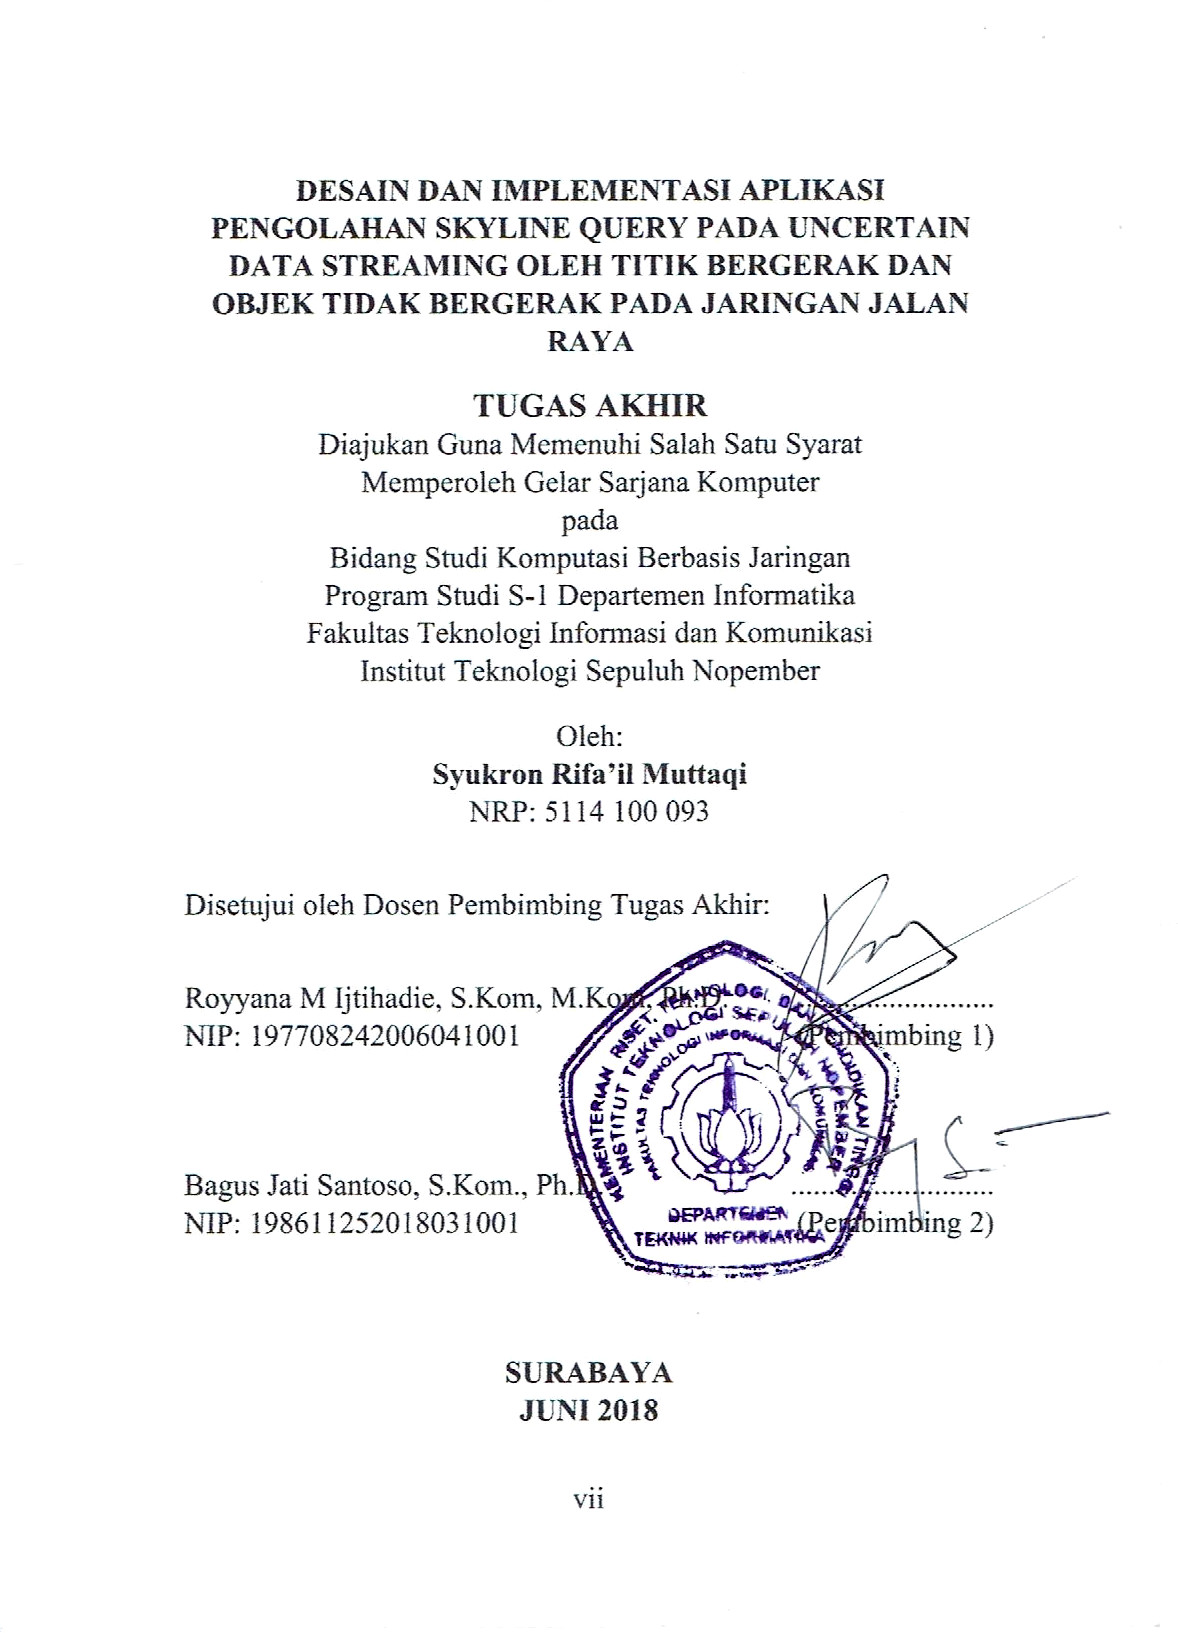
\includegraphics[scale=0.9001]{pengesahan/pengesahan.jpg}}
		\label{figure:lpeng}
	\end{figure}
	
	\cleardoublepage
	% INDONESIAN ABSTRAK
\addcontentsline{toc}{chapter}{ABSTRAK}
\thispagestyle{plain}
\begin{centering}
\centering
\textbf{\MakeUppercase{\judul}}
\end{centering}

\begin{tabular}{ll}
Nama  & : \MakeUppercase{\penulis} \\
NRP & : \nrp \\
Departemen  & : \jurusan FTIK-ITS \\
Pembimbing I  & : \pembimbingSatu \\
Pembimbing II  & : \pembimbingDua
\end{tabular}
\\*[20pt]
\begin{centering}
\textbf{Abstrak}
\end{centering}
\itshape
% BEGIN
\\*[5pt]
Kemajuan ilmu pengetahuan dan teknologi, terutama di bidang analisis data, telah mempengaruhi cara perusahaan dalam menjalankan bisnis, yaitu dengan mengumpulkan data preferensi pelanggan dari data penjualan produk, kemudian memanfaatkannya untuk mendapatkan informasi yang dapat digunakan untuk membuat keputusan bisnis yang tepat. Saat ini, sudah ada penelitian yang mengembangkan strategi pemilihan produk dengan melakukan pencarian $k$-produk yang paling banyak diminati oleh pelanggan bernama \textit{k-Most Promising Products} (k-MPP). Komputasi k-MPP menggunakan dua tipe kueri \textit{skyline}, yaitu \textit{dynamic skyline} dan \textit{reverse skyline}. Sayangnya, komputasi k-MPP tidak mempertimbangkan variabel waktu dalam algoritme perhitungannya dan tidak dapat digunakan untuk memproses kueri berbasis interval waktu.
\\*[5pt]
Tugas Akhir ini bertujuan untuk menjawab permasalahan k-MPP berbasis interval waktu pada data multidimensi dengan serial waktu dengan memodelkan kueri k-MPPTI \textit{(k-Most Promising Products in Time Intervals)} dan merancang kerangka kerja algoritme yang dapat memproses kueri tersebut. Ada tiga jenis algoritme yang dibuat dan dibandingkan, yaitu k-MPPTI (menggunakan kueri \textit{dynamic skyline} dan \textit{reverse skyline}), k-MPPTI NoRSL (menggunakan kueri \textit{dynamic skyline} saja), dan k-MPPTI NoRSL-P (menggunakan teknik komputasi paralel). Efektivitas dan efisiensi algoritme diuji menggunakan data asli dan sintetis.
\\*[5pt]
Hasil uji coba menunjukkan bahwa algoritme k-MPPTI NoRSL memiliki performa yang lebih baik daripada algoritme k-MPPTI karena dapat memberikan hasil kueri dengan waktu eksekusi lima kali lebih cepat dan penggunaan memori satu kali lebih hemat dibandingkan dengan algoritme k-MPPTI.
% END
\rm \\*[5pt]
\textbf{Kata Kunci: \textit{Strategi Pemilihan Produk, Kueri, Dynamic Skyline, Reverse Skyline, Interval Waktu}}


\cleardoublepage

% ENGLISH ABSTRACT
\addcontentsline{toc}{chapter}{ABSTRACT}
\thispagestyle{plain}
\begin{centering}
\textbf{\MakeUppercase{\judulEnglish}}
\end{centering}

\begin{tabular}{ll}
Name  & : \MakeUppercase{\penulis} \\
NRP & : \nrp \\
Major  & : \jurusanEnglish Faculty of IT-ITS \\
Supervisor I  & : \pembimbingSatu \\
Supervisor II  & : \pembimbingDua
\end{tabular}
\\*[20pt]
\begin{centering}
\textbf{Abstract}
\end{centering}
\itshape
% BEGIN
\\*[5pt]
The advancement of science and technology, especially in the data analytics area, has influenced the way manufacturers do businesses by collecting customer preferences from product sales data, then using it to obtain some informations to make the right business decision. Currently, there is a product selection strategy by searching for k-most preferred product by customers, namely k-Most Promising Products (k-MPP). This computation uses two types of skyline queries, dynamic skyline and reverse skyline. Unfortunately, k-MPP computation doesn't consider the time variable and can't process query based on time intervals.
\\*[5pt]
This study aims to answer the k-MPP query based on time intervals in multidimensional time series data with serial time by modeling k-Most Promising Products in Time Intervals (k-MPPTI) query and designing an algorithmic framework for processing the query. There are three types of algorithm built and compared namely k-MPPTI (using both dynamic skyline and reverse skyline queries), k-MPPTI NoRSL (only using dynamic skyline), and k-MPPTI NoRSL-P (using parallel computing techniques). The effectiveness and efficiency of the algorithm was tested using real and synthetic datasets.
\\*[5pt]
\\
Based on the testing results, k-MPPTI NoRSL algorithm has better performance than k-MPPTI algorithm because it provides query results with execution time five times faster and memory usage one-time more efficient than k-MPPTI algorithm.
% END
\rm \\*[5pt]
\textbf{Keywords: \textit{Product Selection Strategy, Query, Dynamic Skyline, Reverse Skyline, Time Interval}}

\cleardoublepage

	\chapter{KATA PENGANTAR}
\indent\indent Puji syukur penulis panjatkan kepada Allah Swt. atas pertolongan dan karunia-Nya sehingga penulis dapat menyelesaikan Tugas Akhir yang berjudul:
\begin{center}
	\textbf{\MakeUppercase{\judul}}.
\end{center}

Penelitian Tugas Akhir ini dilakukan untuk memenuhi salah satu syarat meraih gelar Sarjana di Departemen Informatika, Fakultas Teknologi Informasi dan Komunikasi, Institut Teknologi Sepuluh Nopember Surabaya.

Dengan selesainya Tugas Akhir ini, diharapkan apa yang telah dikerjakan oleh penulis dapat memberikan manfaat bagi perkembangan ilmu pengetahuan, terutama di bidang teknologi informasi, serta bagi diri penulis sendiri selaku peneliti.

Penulis juga mengucapkan banyak terima kasih kepada semua pihak yang telah memberikan dukungan, baik secara langsung maupun tidak langsung, selama penulis mengerjakan Tugas Akhir maupun selama menempuh masa studi antara lain:

\begin{enumerate}
	\item Ibu, Bapak, kedua Adik, Akbar dan Alam, serta segenap keluarga yang senantiasa memberikan perhatian, dukungan, serta kasih sayang yang menjadi semangat dan motivasi bagi diri penulis untuk menyelesaikan Tugas Akhir.
	\item Bapak Bagus Jati Santoso, S.Kom., Ph.D. selaku dosen pembimbing yang telah banyak meluangkan waktu untuk membimbing dan memberikan ilmu, saran, dan motivasi kepada penulis baik selama menempuh masa kuliah maupun selama pengerjaan Tugas Akhir ini.
	\item Ibu Henning Titi Ciptaningtyas, S.Kom., M.Kom. selaku dosen pembimbing yang telah memberikan ilmu dan masukan kepada penulis.
	\item Bapak Darlis Herumurti, S.Kom., M.Kom. selaku Kepala Departemen Informatika ITS pada masa pengerjaan Tugas Akhir, Bapak Radityo Anggoro, S.Kom., M.Sc. selaku koordinator Tugas Akhir, dan segenap dosen dan karyawan Informatika yang telah memberikan ilmu, waktu, dan pengalamannya.
	\item Teman-teman \textit{Sempol Bunda}, Ajeng, Salma, Napik, Bela, dan Yola, yang telah menemani dan mewarnai masa-masa perkuliahan penulis sejak jaman mahasiswa baru.
	\item Seluruh teman-teman Laboratorium Arsitektur dan Jaringan Komputer (AJK), Mas Syukron, Mas Fatih, Nahda, Satria, Awan, Mas Penyok, Fuad, Didin, Hana, Raldo, Aguel, Khawari, Tamtam, Haura, Lia, Sulton, Mail, Yoga, dan Fawwaz, yang telah menemani, mengganggu, dan membantu penulis selama mengerjakan Tugas Akhir di lab.
	\item Teman-teman \textit{Penguasa Kosan}, Ajeng, Salma, Napik, Prames, Kikik, Balqis, Tije, Nilam, dan Rini, yang pernah mengajarkan cara bersenang-senang. 
	\item Emak kos terbaik, Mak Ju, atas segala bantuannya selama ini dan teman-teman kosan 36, Jakiya, Mutek, Marisa, Mbak Tatak, Alya, Firda, dan Anca.
	\item Teman-teman \textit{Data Engineers}, Hana dan Rio, sebagai teman seperjuangan dan seperbimbingan.
	\item Seluruh teman-teman TC 2015 yang tidak bisa penulis sebutkan satu persatu namanya.
\end{enumerate}

Penulis mohon maaf apabila masih ada kekurangan pada Tugas Akhir ini. Penulis juga mengharapkan kritik dan saran yang membangun untuk pembelajaran dan perbaikan di kemudian hari. Semoga melalui Tugas Akhir ini Penulis dapat memberikan kontribusi dan manfaat yang sebaik-baiknya. \\ \\ \\

\hfill Surabaya, Juni \tahun \\ \\ \\

\hfill \penulis \\
\cleardoublepage

	\tableofcontents
	\cleardoublepage
	\listoftables
	\cleardoublepage
	\listoffigures
	\cleardoublepage
	\lstlistoflistings
	\cleardoublepage
	
	\mainmatter
	\chapter{PENDAHULUAN}
\tab Pada bab ini dijelaskan latar belakang, rumusan masalah, batasan masalah, tujuan, manfaat, metodologi dan sistematika penulisan Tugas Akhir.

\section{Latar Belakang}
\tab Pesatnya kemajuan ilmu pengetahuan dan teknologi di bidang analisis data telah mempengaruhi cara perusahaan dalam berbisnis, yakni dengan mengumpulkan data-data penjualan, riset pasar, logistik, atau biaya transportasi, kemudian menggunakannya untuk membuat keputusan bisnis yang lebih baik. Seorang analis data atau analis bisnis dapat mengumpulkan data preferensi pelanggan terhadap fitur-fitur produk perusahaan tersebut dari data penjualan yang dimiliki. Selain itu, maraknya penggunaan situs web untuk menjual produk secara \textit{online} juga memungkinkan analis mengumpulkan data preferensi pelanggan terhadap fitur produk perusahaan lain.

Dengan memanfaatkan data penjualan produk dan data preferensi pelanggan, sebuah perusahaan dapat mendapatkan informasi yang dapat digunakan untuk membuat keputusan bisnis yang tepat. Misalnya, dengan mendapatkan informasi $k$-produk apa saja yang paling diminati oleh pelanggan beserta fitur-fiturnya, perusahaan dapat menentukan harga produk baru yang akan diluncurkan atau menentukan fitur-fitur apa yang hendak diunggulkan dari produk baru yang akan diluncurkan. 

\pagebreak
Saat ini, sudah ada penelitian yang mengembangkan strategi pemilihan produk dengan melakukan pencarian $k$-produk yang paling banyak diminati oleh pelanggan. Islam dan Liu (2010) memodelkannya sebagai kueri \textit{k-Most Promising Products} (k-MPP), serta membuat kerangka kerja algoritme untuk memproses kueri tersebut \cite{kmpp}. Komputasi k-MPP menggunakan dua tipe kueri \textit{skyline}, yaitu \textit{dynamic skyline} \cite{dynamic-skyline} dan \textit{reverse skyline} \cite{reverse-skyline}. Kueri \textit{dynamic skyline} digunakan untuk mengambil data produk terbaik berdasarkan sudut pandang pelanggan, sedangkan kueri \textit{reverse skyline} digunakan untuk mengambil data pelanggan potensial berdasarkan sudut pandang produk atau perusahaan.

Kelemahan dari strategi pemilihan produk k-MPP adalah tidak adanya pertimbangan variabel waktu, sehingga hasilnya tidak valid untuk digunakan sebagai bahan pertimbangan pembuat keputusan di masa yang akan datang, misalnya salah satu dari hasil pencarian $k$-produk yang unggul ternyata sudah tidak diproduksi lagi saat ini. 

Selain itu, komputasi k-MPP tidak dapat memproses kueri berbasis interval waktu. Pertanyaan yang mungkin akan diajukan adalah \textit{“$k$-produk apa saja yang paling banyak diminati oleh pelanggan pada bulan Februari hingga September?”}. Dalam hal ini, bulan Februari hingga September disebut dengan interval waktu kueri dan data yang berbasis interval waktu disebut dengan data \textit{time series} atau serial waktu.

Waktu adalah variabel penting yang harus dipertimbangkan dalam analisis data supaya informasi yang didapatkan valid dengan kondisi yang sebenarnya. Sebagai ilustrasi, produk A adalah produk yang paling banyak diminati oleh pelanggan pada bulan Januari hingga Juni, namun pada bulan Juli hingga September posisinya diungguli oleh produk B yang lebih diminati pelanggan. Pada bulan Oktober, produk B tidak diproduksi lagi karena suatu alasan, sehingga produk A kembali diminati pelanggan.  

Berdasarkan ilustrasi di atas, produk yang paling unggul berdasarkan kueri k-MPP biasa adalah produk B karena produk B pernah mengungguli produk A, padahal produk B sudah tidak diproduksi lagi saat ini. Hal ini terjadi karena komputasi k-MPP hanya mempertimbangkan skor kontribusi pasar yang dihitung dari banyaknya jumlah pelanggan yang lebih menyukai produk tersebut daripada produk lainnya, tanpa mempertimbangkan variabel waktu.

Sedangkan jika berdasarkan kueri dengan interval waktu Januari hingga Juli, maka produk yang paling unggul adalah produk A; jika berdasarkan kueri dengan interval waktu Juli hingga Agustus, maka produk yang paling unggul adalah produk B; dan jika berdasarkan kueri dengan interval waktu Januari hingga Desember, maka produk yang paling unggul adalah produk A karena masa ketika produk A unggul lebih lama daripada produk B.

Tugas Akhir ini bertujuan untuk menjawab permasalahan k-MPP berbasis interval waktu pada data multidimensi dengan serial waktu dengan memodelkan kueri k-MPPTI \textit{(k-Most Promising Products in Time Intervals)}, serta merancang kerangka kerja algoritme yang dapat memproses kueri tersebut. Algoritme diimplementasikan menggunakan teknik komputasi paralel supaya pemrosesan data menjadi lebih cepat. Efektivitas dan efisiensi algoritme diuji menggunakan data asli dan dataset sintetis.

\section{Rumusan Masalah}
\tab Rumusan masalah yang diangkat dalam Tugas Akhir ini adalah sebagai berikut:
\begin{enumerate}
	\item Bagaimana desain dan implementasi struktur data dan algoritme untuk \problemm?
	\item Bagaimana kinerja dari struktur data dan algoritme yang dibangun untuk \problemm?
	\item Bagaimana strategi yang optimal untuk meningkatkan efisiensi komputasi \textit{k-Most Promising Products} (k-MPP) berbasis interval waktu pada data multidimensi dengan serial waktu?
\end{enumerate}

\section{Batasan Masalah}
\tab Permasalahan yang dibahas pada Tugas Akhir ini memiliki beberapa batasan sebagai berikut:
\begin{enumerate}
	\item Struktur data dan algoritme dalam komputasi \textit{k-Most Promising Products} (k-MPP) berbasis interval waktu hanya dapat menyimpan dan memproses nilai numerik.
	\item Implementasi struktur data dan algoritme menggunakan bahasa pemrograman Python.
	\item \textit{Dataset} yang digunakan adalah data asli dan sintetis.
\end{enumerate}

\section{Tujuan}
\tab Tujuan dari Tugas Akhir ini adalah sebagai berikut:

\begin{enumerate}
	\item Merancang dan mengimplementasikan struktur data dan algoritme untuk \problemm.
	\item Mengevaluasi kinerja dari struktur data dan algoritme yang dibangun untuk \problemm.
	\pagebreak
	\item Mengimplementasikan strategi yang optimal untuk meningkatkan efisiensi komputasi \textit{k-Most Promising Products} (k-MPP) berbasis interval waktu pada data multidimensi dengan serial waktu.
\end{enumerate}

\section{Manfaat}
\tab Manfaat yang diharapkan dari penulisan Tugas Akhir ini adalah untuk mengetahui struktur data dan algoritme yang tepat untuk \problemm secara optimal dan efisien.

Selain itu, Tugas Akhir ini juga diharapkan dapat memberikan kontribusi pada perkembangan ilmu pengetahuan dan teknologi informasi karena algoritme ini dapat digunakan dalam berbagai hal, khususnya bagi perusahaan untuk membuat bisnisnya menjadi lebih baik dan tepat sasaran.

\section{Metodologi}
\tab Metodologi yang digunakan dalam pengerjaan Tugas Akhir ini adalah sebagai berikut:
\begin{enumerate}
	
	\item Penyusunan proposal Tugas Akhir
	
	\tab Tahap awal untuk memulai pengerjaan Tugas Akhir adalah penyusunan proposal Tugas Akhir yang berisi gagasan untuk \problemm. Proposal ini berisi tentang deskripsi pendahuluan dari Tugas Akhir yang akan dibuat, terdiri atas hal yang menjadi latar belakang diajukannya usulan Tugas Akhir, rumusan masalah yang diangkat, batasan masalah, tujuan, dan manfaat dari pembuatan Tugas Akhir. Selain itu, dijabarkan pula tinjauan pustaka yang digunakan sebagai referensi pendukung pembuatan Tugas Akhir.	
	
	\item Studi literatur
	
	\tab Pada tahap ini dilakukan pencarian informasi dan literatur mengenai metode yang dapat digunakan dalam merancang dan mengimplementasikan struktur data dan algoritme untuk \problemm. Informasi-informasi tersebut bisa didapatkan dari buku, jurnal, maupun internet.
	
	\item Analisis dan perancangan perangkat lunak
	
	\tab Pada tahap ini dilakukan analisis dan perancangan struktur data dan algoritme yang digunakan untuk \problemm berdasarkan literatur yang telah
	dipelajari.
	
	\item Implementasi perangkat lunak
	
	\tab Pada tahap ini dilakukan implementasi atau realiasi dari hasil analisis dan perancangan struktur data dan algoritme yang telah dibuat ke dalam bentuk program.
	
	\item Uji coba dan evaluasi
	
	\tab Pada tahap ini dilakukan uji coba dari struktur data dan algoritme yang telah diimplementasikan. Pengujian akan dilakukan dengan dua cara, yaitu:
	
	\begin{enumerate}
		\item Pengujian waktu eksekusi \textit{(runtime)}
		
		\tab Pengujian yang berfokus pada waktu eksekusi dari struktur data dan algoritme yang dibangun untuk \problemm.
		
		\item Pengujian penggunaan memori \textit{(memory usage)}
		
		\tab Pengujian yang berfokus pada konsumsi memori dari struktur data dan algoritme yang dibangun untuk \problemm.
	\end{enumerate}
	
	\tab Setelah dilakukan uji coba, maka dilakukan evaluasi terhadap kinerja struktur data dan algoritme yang telah diimplementasikan, dengan harapan dapat diperbaiki ke depannya.
	
	\item Penyusunan buku Tugas Akhir
	
	\tab Pada tahap ini dilakukan penyusunan buku Tugas Akhir yang berisi dokumentasi pengerjaan dan laporan hasil pengerjaan Tugas Akhir.
	
\end{enumerate}

\section{Sistematika Penulisan}
Berikut adalah sistematika penulisan buku Tugas Akhir:
\begin{enumerate}
	\item BAB I: PENDAHULUAN
	
	\tab Bab ini berisi latar belakang, rumusan masalah, batasan masalah, tujuan, manfaat, metodologi dan sistematika penulisan Tugas Akhir.
	
	\item BAB II: TINJAUAN PUSTAKA
	
	\tab Bab ini berisi dasar teori mengenai permasalahan dan algoritme penyelesaian yang digunakan dalam Tugas Akhir
	
	\item BAB III: ANALISIS DAN PERANCANGAN SISTEM
	
	\tab Bab ini berisi analisis dan perancangan struktur data dan algoritme yang digunakan dalam penyelesaian permasalahan.
	
	\item BAB IV: IMPLEMENTASI
	
	\tab Bab ini berisi implementasi berdasarkan analisis dan perancangan struktur data dan algortime yang telah dilakukan pada tahap analisis dan perancangan sistem.
	
	\item BAB V: UJI COBA DAN EVALUASI
	
	\tab Bab ini berisi uji coba dan evaluasi dari hasil implementasi yang telah dilakukan pada tahap implementasi.
	
	\pagebreak
	\item BAB VI: PENUTUP
	
	\tab Bab ini berisi kesimpulan dan saran yang didapat dari hasil uji coba dan evaluasi yang telah dilakukan.
	
\end{enumerate}

\cleardoublepage

	% Masing-masing dasar teori terdiri dari:
% - What - definisi, contoh
% - Why - alasan digunakan
% - How - Penggunaan dalam tugas akhir

\chapter{TINJAUAN PUSTAKA} \label{chap:tinjauan-pustaka}
\tab Bab ini menjelaskan dasar teori yang digunakan dalam analisis, perancangan, dan implementasi struktur data dan algoritme untuk menjawab permasalahan \textit{k-Most Promising Products} ($k$-MPP) berbasis interval waktu pada data multidimensi dengan serial waktu yang diangkat dalam Tugas Akhir ini. 

\section{Daftar Notasi}
\tab Tabel \ref{tab:daftar-notasi-1} menunjukkan daftar notasi yang digunakan untuk memudahkan beberapa penjelasan pada bab ini berikut dengan deskripsinya.

\begin{longtable}{| p{3cm} | p{6cm} |} 
	\caption{Daftar Notasi (1) \label{tab:daftar-notasi-1}}\\
	\hline
	\textbf{Notasi} & \textbf{Deskripsi}\\ \hline
	\endfirsthead
	\hline
	\textbf{Notasi} & \textbf{Deskripsi}\\ \hline
	\endhead
	$P$ & \textit{Dataset} produk\\ \hline
	$C$ & \textit{Dataset} pelanggan (preferensi pelanggan)\\ \hline
	$D$ & $P \cup C$ \\ \hline
	$ob$ & Sebuah objek data pada $D$\\ \hline
	$ob_1 \prec ob_2$ & Objek data $ob_1$ mendominasi $ob_2$\\ \hline
	$ob_1 \prec_{ob_3} ob_2$ & Objek data $ob_1$ mendominasi $ob_2$ berdasarkan $ob_3$\\ \hline
	$p$ & Sebuah produk dalam $P$, $p \in P$\\ \hline
	$c$ & Seorang pelanggan dalam $C$, $c \in C$\\ \hline
	$d$ & Jumlah dimensi pada $D$\\ \hline
	$i$ & Dimensi ke-1, ..., $d$\\ \hline
	$j$ & Timestamp ke-1, 2, ..., dst\\ \hline
	$O$ & \textit{Orthant} atau daerah pada komputasi \textit{reverse skyline}\\ \hline
	$m$ & \textit{Midpoint} antar produk pada komputasi \textit{reverse skyline}\\ \hline
	$DSL(c)$ & Hasil \textit{dynamic skyline} dari pelanggan $c$\\ \hline
	$RSL(p)$ & Hasil \textit{reverse skyline} dari produk $p$\\ \hline
	$Pr(c, p|P)$ & Probabilitas produk $p$ dibeli oleh pelanggan $c$ \\ \hline
	$E(C, p|P)$ & Kontribusi pasar $p$\\ \hline
	$E(C, P'|P)$ & Kontribusi pasar subset $P'$ dari $P$ \\ \hline
	$k-MPP$ & \textit{k-Most Promising Products} \\ \hline
\end{longtable}

\section{Data}
\tab Data merupakan elemen yang esensial dalam sebuah sistem informasi. Data adalah informasi faktual (seperti pengukuran atau statistik) yang digunakan sebagai dasar untuk analisis, diskusi, maupun perhitungan \cite{data}. 

Meski begitu, data mentah tidaklah berarti dan harus diproses terlebih dahulu supaya menghasilkan informasi yang bermanfaat. Sehingga, dibutuhkanlah sebuah algoritme pemrosesan data yang menerima data sebagai \textit{input}, kemudian memprosesnya menjadi informasi tertentu sesuai dengan kebutuhan pengguna dan mengeluarkannya sebagai \textit{output}.

\subsection{Data Multidimensi}
\tab Model data multidimensi adalah sebuah cara pandang yang melihat data dari berbagai sudut pandang atau dimensi. Model data ini memiliki struktur yang disesuaikan untuk mengoptimalkan analisis berdasarkan data dari \textit{relational database} dan diolah sehingga informasi dapat dikategorikan. Model data multidimensi merupakan variasi dari model relasional yang mengunakan struktur multidimensi untuk menyusun data dan menjelaskan relasi antar data.

Struktur multidimensi merepresentasikan dimensi-dimensi data dalam bentuk kubus. Jika sebuah data multidimensi memiliki lebih dari tiga dimensi, maka disebut dengan \textit{hypercube} \cite{multidimensional-database}. Dalam implementasinya, data multidimensi disajikan dalam bentuk \textit{array} multidimensi yang masing-masing nilai dalam selnya dapat diakses menggunakan sebuah indeks.

Data multidimensi banyak digunakan untuk analisis. Selama beberapa tahun terakhir, konsep data multidimensi telah menjadi hal yang fundamental dalam sistem pengambil keputusan, seperti sistem \textit{data warehouse} \cite{multidimensional-database}.

\subsection{Data Serial Waktu}
\tab Data \textit{time series} atau serial waktu adalah nilai-nilai suatu variabel yang berurutan menurut waktu. Data \textit{time series} memiliki nilai dan \textit{timestamp}, sehingga data diurutkan berdasarkan waktu atau \textit{timestamp}-nya.

\newcolumntype{C}{>{\centering\arraybackslash}p{1.5em}}
\begin{table}[h]
	\small
	\centering
	\caption{Contoh Data \textit{Time Series} \label{tab:data-time-series}}
	\begin{tabular}{|C|C|C|C|C|C|}
		\hline
		\multirow{2}{*}{\textbf{id}} & \multicolumn{5}{c|}{\textbf{timestamp}}\\
		\cline{2-6}
		& \textbf{1} & \textbf{2} & \textbf{3} & \textbf{4} & \textbf{5} \\ \hline \hline		
		$s_1$ & 8 & 2 & 5 & 10 & 12 \\ \hline
		$s_2$ & 14 & 4 & 10 & 7 & 8 \\ \hline
		$s_3$ & 15 & 6 & 11 & 7 & 3 \\ \hline
		$s_4$ & 3 & 8 & 12 & 9 & 13 \\ \hline
		$s_5$ & 15 & 9 & 10 & 2 & 7 \\ \hline
	\end{tabular}
\end{table}

Pada Tabel \ref{tab:data-time-series}, diberikan contoh sebuah data \textit{time series} $S$. Supaya sederhana, kita asumsikan bahwa \textit{timestamp} adalah bilangan bulat positif. Nilai $s_1 \in S$ pada \textit{timestamp} $j$ dinotasikan sebagai $s_1[j]$, sehingga \textit{time series} $s_1$ jika ditulis secara berurutan menjadi $s_1[1], s_1[2],..$ , dan seterusnya \cite{time-series}.

\subsection{Data Multidimensi dengan Serial Waktu}
\tab Untuk menjawab permasalahan yang diangkat pada Tugas Akhir ini, data yang digunakan merupakan penggabungan dari kedua jenis data di atas, yaitu data multidimensi dengan serial waktu.

Data multidimensi dengan serial waktu adalah data \textit{multi-attribute} yang memiliki \textit{timestamp} dan berurutan menurut waktu. Pada Tabel \ref{tab:data-multidimensi-ts-1}, diberikan contoh sebuah data produk yang memiliki nilai atribut dan \textit{timestamp}.

\newcolumntype{C}{>{\centering\arraybackslash}p{1.2em}}
\begin{table}[h]
	\small
	\centering
	\caption{Contoh Data Multidimensi dengan Serial Waktu (1) \label{tab:data-multidimensi-ts-1}}
	\begin{tabular}{|C|C|C|C|C|C|C|C|C|C|C|}
		\hline
		\multirow{3}{*}{\textbf{id}} & \multicolumn{10}{c|}{\textbf{timestamp}}\\ \cline{2-11}
		& \multicolumn{2}{c|}{\textbf{1}} & \multicolumn{2}{c|}{\textbf{2}} & \multicolumn{2}{c|}{\textbf{3}} & \multicolumn{2}{c|}{\textbf{4}} & \multicolumn{2}{c|}{\textbf{5}}\\ \cline{2-11}
		& \textbf{$d_1$} & \textbf{$d_2$} & \textbf{$d_1$} & \textbf{$d_2$} & \textbf{$d_1$} & \textbf{$d_2$} & \textbf{$d_1$} & \textbf{$d_2$} & \textbf{$d_1$} & \textbf{$d_2$}\\ \hline
		\hline		
		$p_1$ & 2 & 8 & 2 & 8 & 2 & 8 & 2 & 8 & 2 & 8 \\ \hline
		$p_2$ & - & - & - & - & - & - & 4 & 10 & 4 & 10 \\ \hline
		$p_3$ & 6 & 11 & 6 & 11 & 6 & 11 & - & - & - & - \\ \hline
		$p_4$ & - & - & - & - & - & - & - & - & 8 & 12 \\ \hline
		$p_5$ & 9 & 10 & 9 & 10 & 9 & 10 & 9 & 10 & - & - \\ \hline
	\end{tabular}
\end{table}

Contoh data pada Tabel \ref{tab:data-multidimensi-ts-1} sekilas hampir sama dengan data pada Tabel \ref{tab:data-time-series}, namun memiliki atribut atau dimensi lebih dari satu. Jika asumsinya nilai pada atribut data selalu tetap, maka data pada Tabel \ref{tab:data-multidimensi-ts-1} dapat ditulis menjadi Tabel \ref{tab:data-multidimensi-ts}. Timestamp yang banyak dan berurutan dapat ditulis menjadi interval waktu (\textit{timestamp in - timestamp out}), dinotasikan dengan $[i:j]$. Interval waktu menggambarkan bahwa sebuah data memiliki waktu hidup tertentu.

\newcolumntype{C}{>{\centering\arraybackslash}p{2.5em}}
\begin{table}[h]
	\small
	\centering
	\caption{Contoh Data Multidimensi dengan Serial Waktu (2) \label{tab:data-multidimensi-ts}}
	\begin{tabular}{|C|C|C|C|C|}
		\hline
		\textbf{id} & \textbf{ts\_in} & \textbf{ts\_out} & \textbf{dim1} & \textbf{dim2}\\ \hline \hline
		$p_1$ & 1 & 8 & 2 & 8 \\ \hline
		$p_2$ & 4 & 14 & 4 & 10\\ \hline
		$p_3$ & 1 & 3 & 6 & 11\\ \hline
		$p_4$ & 5 & 15 & 8 & 12\\ \hline
		$p_5$ & 1 & 4 & 9 & 10\\ \hline
	\end{tabular}
\end{table}

Data yang digunakan pada Tugas Akhir ini adalah dataset produk $P$ dan pelanggan $C$. Ilustrasinya, setiap produk $p \in P$ memiliki waktu kapan ia pertama kali diproduksi dan kapan ia tidak diproduksi lagi, sedangkan setiap pelanggan $c \in C$ memiliki waktu kapan ia lahir dan kapan ia meninggal dunia.

\section{\textit{Skyline}}
\tab Komputasi \textit{skyline} telah menarik perhatian yang cukup besar dari peneliti sejak diperkenalkan pada komunitas basis data \cite{skyline}, terutama mengenai metode progresif yang dapat mengembalikan hasil kueri dengan cepat tanpa perlu membaca keseluruhan data \cite{dynamic-skyline}. Tujuan dari komputasi \textit{skyline} adalah mencari data yang “menarik” dari suatu himpunan data \cite{skyline}, yaitu data yang tidak didominasi oleh data lain atau data yang paling unggul.

Diberikan \textit{dataset} produk $P$ yang setiap datanya direpresentasikan sebagai titik $d$-dimensi. Sebuah titik $p_1$ dikatakan mendominasi titik lain $p_2$, dinotasikan dengan  $p_1 \prec p_2$, jika nilai $p_1$ tidak lebih besar dari $p_2$ pada semua dimensi dan ada nilai $p_1$ yang lebih kecil dari $p_2$ minimal pada satu dimensi. Secara matematika, relasi $p_1 \prec p_2$ dapat terbentuk jika dan hanya jika:
\[\text{(a)} \tab p_1^i \leq p_2^i, \forall i \in [1, ..., d]\] 
\[\text{(b)} \tab p_1^i < p_2^i, \exists i \in [1, ..., d]\]

Misalnya, seseorang ingin mencari produk \textit{smartphone} terbaik, yaitu \textit{smartphone} yang memiliki harga termurah dan memiliki resolusi kamera terbesar. Pada Tabel \ref{tab:dataset}, diberikan data produk $P$ yang memiliki atribut resolusi kamera ($dim_1$) dan harga ($dim_2$). Setiap datanya direpresentasikan sebagai titik pada bidang dua dimensi, yakni sumbu $x$ adalah resolusi kamera dan sumbu $y$ adalah harga \textit{smartphone}.

\begin{figure}[h]
	\centering
	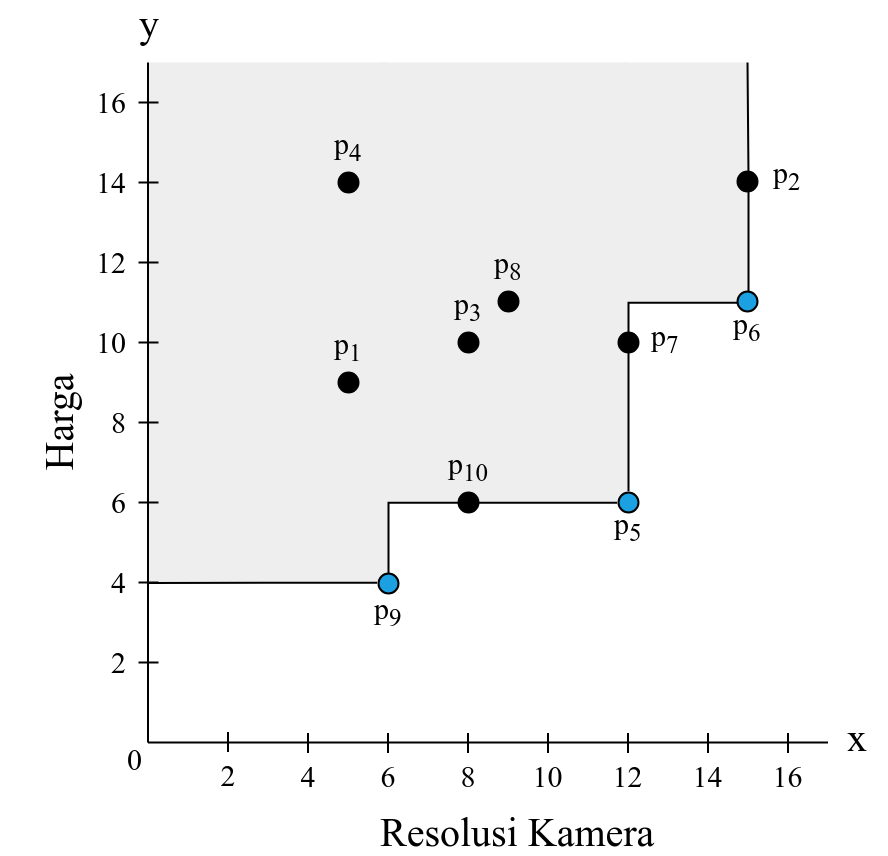
\includegraphics[width=6cm]{assets/img/bab2/skyline.png}
	\caption{Titik Skyline dari Data Produk pada Tabel \ref{tab:dataset}}
	\label{fig:skyline}
\end{figure}

Berdasarkan Gambar \ref{fig:skyline}, produk \textit{smartphone} yang terbaik adalah $p_5$, $p_6$, dan $p_9$ karena tidak ada titik yang lebih baik dari titik-titik tersebut pada semua dimensi, sedangkan produk $p_{10}$ tidak dapat menjadi \textit{skyline} karena didominasi oleh produk $p_5$ pada dimensi $x$. Begitu juga produk $p_7$ yang didominasi $p_5$ pada dimensi $y$ dan produk $p_2$ yang didominasi $p_6$ pada dimensi $y$. Produk $p_5$, $p_6$, dan $p_9$ disebut dengan titik \textit{skyline} atau \textit{skyline point}.

Saat ini, komputasi \textit{skyline} telah banyak digunakan sebagai operator pengambil keputusan multikriteria dan perencanaan bisnis \cite{dynamic-skyline-2}. Ada beberapa pengembangan dari komputasi \textit{skyline}, seperti \textit{dynamic skyline} dan \textit{reverse skyline}.  

\section{Dominansi Dinamis}

\tab Berdasarkan definisi "\textit{Skyline}" yang telah dijelaskan pada sub-bagian sebelumnya, jika diberikan \textit{dataset} yang sama, maka hasil \textit{skyline} dari \textit{dataset} tersebut pasti akan selalu sama. Oleh karena itu, para ahli juga menyebut \textit{original skyline} sebagai \textit{static skyline} \cite{dynamic-skyline-2}.

Ada suatu kasus ketika perhitungan \textit{skyline} didasarkan pada titik kueri. Jika diberikan \textit{dataset} yang sama, namun titik kuerinya berbeda, maka hasil \textit{skyline}-nya pun berbeda tergantung pada titik kueri. \textit{Skyline} ini disebut dengan \textit{dynamic skyline} karena memiliki sifat dominansi dinamis. 

Diberikan \textit{dataset} produk $P$ dan \textit{dataset} pelanggan (preferensi pelanggan) $C$ yang setiap datanya direpresentasikan sebagai objek data $d$-dimensi dan hanya dapat menyimpan nilai numerik pada setiap dimensinya. Data produk dan pelanggan pada dimensi ke-$i$ dinotasikan sebagai $p^i$ dan $c^i$, $i \leq d$. Untuk menggambarkan objek data secara umum digunakan notasi $ob$.

Suatu objek data $ob_1$ dikatakan mendominasi objek data $ob_2$ secara dinamis berdasarkan objek data $ob_3$, dinotasikan dengan $ob_1 \prec_{ob_3} ob_2$, jika nilai $ob_1$ dekat dengan $ob_3$ pada semua dimensi dan ada nilai $ob_1$ yang lebih dekat dengan $ob_3$ dibandingkan nilai $ob_2$ dengan $ob_3$ minimal pada satu dimensi. Secara matematika, relasi $ob_1 \prec_{ob_3} ob_2$ terbentuk jika dan hanya jika:
\begin{equation}\label{eq:syarat-dominansi-dinamis}
\begin{split}
\text{(a)} \tab |ob_3^i - ob_1^i| \leq |ob_3^i - ob_2^i|, \forall i \in [1, ..., d] \\
\text{(b)} \tab |ob_3^i - ob_1^i| < |ob_3^i - ob_2^i|, \exists i \in [1, ..., d]
\end{split}
\end{equation}

Pada Tabel \ref{tab:dataset}, diberikan contoh \textit{dataset} produk dan preferensi pelanggan. Berdasarkan preferensi pelanggan $c_1$, produk $p_1$ dikatakan mendominasi produk $p_2$, dinotasikan dengan $p_1 \prec_{c_1} p_2$, karena memenuhi kedua syarat dominansi dinamis yakni (a) $|c_1^1 - p_1^1| = |5-5| = 0 \leq |c_1^1 - p_2^1| = |5-15| = 10$ dan (b) $|c_1^2 - p_1^2| = |2-9| = 7 < |c_1^2 - p_2^2| = |2-14| = 12$.

\newcolumntype{C}{>{\centering\arraybackslash}p{2.5em}}
\begin{table}[H]
	\caption{Contoh \textit{Dataset}\\(a) Produk $P$ dan (b) Preferensi Pelanggan $C$ \label{tab:dataset}}
	\begin{subtable}{.5\linewidth}
		\small
		\centering
		\caption{}
		\begin{tabular}{|C|C|C|}
			\hline
			\textbf{id} & \textbf{dim1} & \textbf{dim2}\\ \hline \hline
			$p_1$ & 5 & 9\\ \hline
			$p_2$ & 15 & 14\\ \hline
			$p_3$ & 8 & 10\\ \hline
			$p_4$ & 5 & 14\\ \hline
			$p_5$ & 12 & 6\\ \hline
			$p_6$ & 15 & 11\\ \hline
			$p_7$ & 12 & 10\\ \hline
			$p_8$ & 9 & 11\\ \hline
			$p_9$ & 6 & 4\\ \hline
			$p_{10}$ & 8 & 6\\ \hline
		\end{tabular}
	\end{subtable}%
	\begin{subtable}{.5\linewidth}
		\small
		\centering
		\caption{}
		\begin{tabular}{|C|C|C|}
			\hline
			\textbf{id} & \textbf{dim1} & \textbf{dim2}\\ \hline \hline
			$c_1$ & 5 & 2\\ \hline
			$c_2$ & 8 & 10\\ \hline
			$c_3$ & 15 & 10\\ \hline
			$c_4$ & 9 & 7\\ \hline
			$c_5$ & 10 & 12\\ \hline
			$c_6$ & 12 & 14\\ \hline
			$c_7$ & 7 & 13\\ \hline
			$c_8$ & 15 & 8\\ \hline
			$c_9$ & 5 & 5\\ \hline
			$c_{10}$ & 10 & 5\\ \hline
		\end{tabular}
	\end{subtable} 
\end{table}

Sebaliknya, jika berdasarkan preferensi pelanggan $c_6$, maka produk $p_2$-lah yang mendominasi $p_1$, dinotasikan dengan $p_2 \prec_{c_6} p_1$, karena (a) $|c_6^1 - p_2^1| = |12-15| = 3 \leq |c_6^1 - p_1^1| = |12-5| = 7$ dan (b) $|c_6^2 - p_2^2| = |14-14| = 0 < |c_6^2 - p_1^2| = |14-9| = 5$. Dalam hal ini, preferensi pelanggan disebut dengan titik kueri karena dapat mempengaruhi sifat dominansi antar produk.

Mengambil contoh lain, produk $p_1$ tidak mendominasi $p_2$ berdasarkan pelanggan $c_3$ karena ada salah satu syarat dominansi dinamis yang tidak terpenuhi, (a) $|c_3^1 - p_1^1| = |15-5| = 10 \nleq |c_3^1 - p_2^1| = |15-15| = 0$ dan (b) $|c_3^2 - p_1^2| = |10-9| = 1 < |c_3^2 - p_2^2| = |10-14| = 4$. Produk $p_1$ dan $p_2$ dikatakan saling mendominasi berdasarkan pelanggan $c_2$.

\section{\textit{Dynamic Skyline}}
\tab Kueri \textit{dynamic skyline} dalam komputasi $k$-MPP digunakan untuk mencari produk terbaik dari sudut pandang pelanggan \cite{kmpp}, sehingga yang menjadi titik kueri adalah pelanggan. \textit{Dynamic skyline} \cite{dynamic-skyline} dari seorang pelanggan $c_1 \in C$, dinotasikan dengan $DSL(c_1)$, berisi semua produk $p_1 \in P$ yang tidak didominasi oleh produk lain $p_2 \in P$ berdasarkan preferensi pelanggan $c_1$, $p_2 \nprec_{c_1} p_1$.

\textit{Dynamic skyline} dapat dihitung menggunakan algoritme komputasi \textit{skyline} tradisional \cite{skyline}, yaitu mentransformasikan semua titik $p \in P$ ke ruang data baru dengan menganggap titik kueri $c$ sebagai titik asal dan jarak abolut titik $p$ ke $c$ digunakan sebagai fungsi pemetaan seperti yang ditunjukkan pada Gambar \ref{fig:dsl}. Fungsi pemetaan $f^i$ didefinisikan sebagai $f^i (p^i) = |c^i-p^i|$.

Menggunakan \textit{dataset} pada Tabel \ref{tab:dataset}, \textit{dynamic skyline} dari pelanggan $c_4$ adalah $DSL(c_4) = \{p_8, p_{10}\}$, karena produk tersebut tidak didominasi oleh produk lain berdasarkan preferensi pelanggan $c_4$. Berbeda halnya dengan $c_{10}$ yang memiliki hasil \textit{dynamic skyline} $DSL(c_{10}) = \{p_5, p_8, p_{10}\}$.

\begin{figure}[h]
	\centering
	\begin{subfigure}{.5\textwidth}
		\centering
		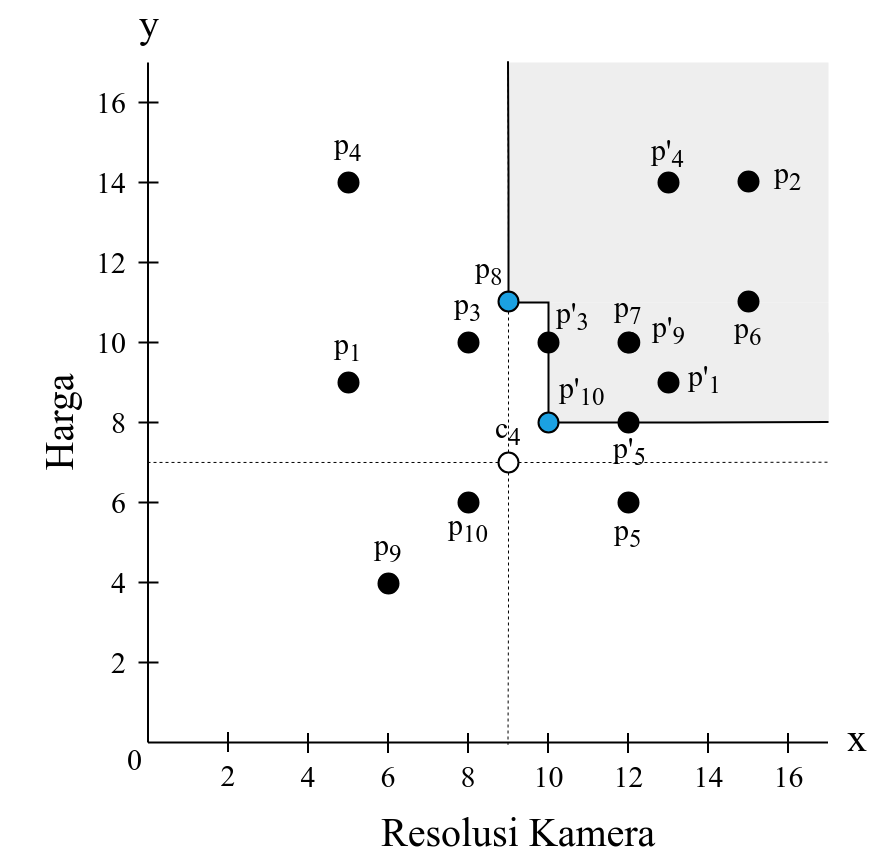
\includegraphics[height=5cm]{assets/img/bab2/dsl-1.png}
		\caption{}
	\end{subfigure}%
	\begin{subfigure}{.5\textwidth}
		\centering
		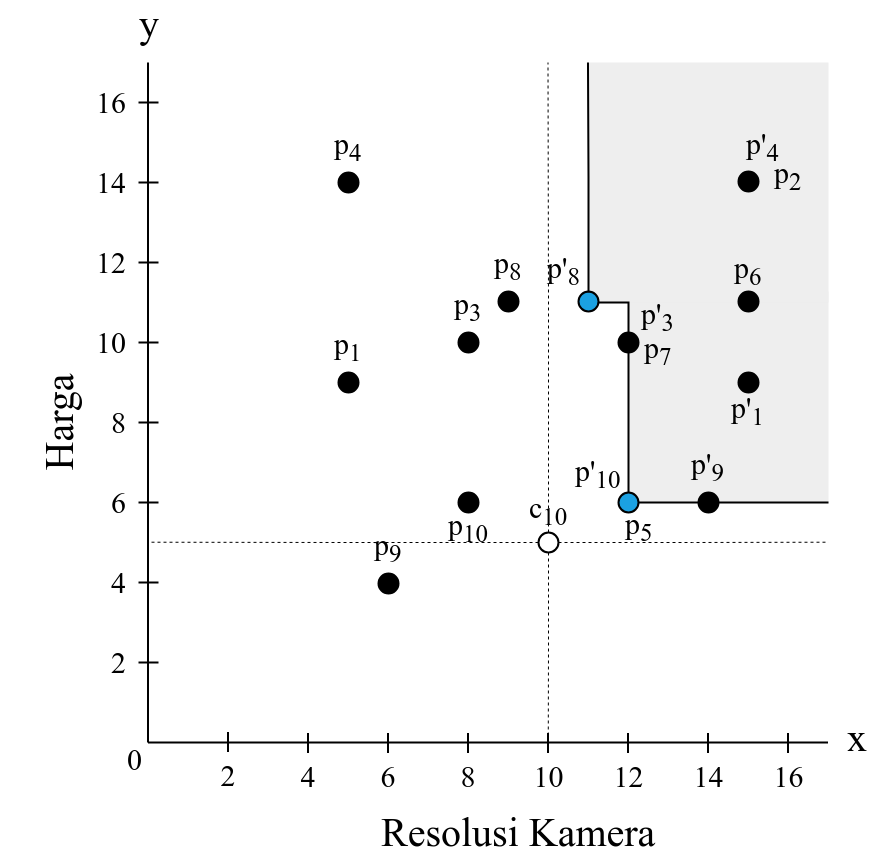
\includegraphics[height=5cm]{assets/img/bab2/dsl-2.png}
		\caption{}
	\end{subfigure}
	\caption{(a) Komputasi \textit{Dynamic Skyline} dari Pelanggan $c_{4}$ dan (b) \textit{Dynamic Skyline} dari Pelanggan $c_{10}$}
	\label{fig:dsl}
\end{figure}

\section{\textit{Reverse Skyline}}
\tab Dalam komputasi $k$-MPP, kueri \textit{reverse skyline} digunakan untuk mencari pelanggan potensial dari sudut pandang produsen \cite{kmpp}, sehingga yang menjadi titik kueri adalah produk. \textit{Reverse skyline} \cite{reverse-skyline} dari sebuah produk $p_1 \in
P$, dinotasikan dengan $RSL(p_1)$, berisi semua pelanggan $c \in C$ yang memiliki $p_1$ pada hasil \textit{dynamic skyline}-nya.

Ada beberapa tahapan yang harus dilakukan dalam komputasi \textit{reverse skyline} \cite{kmpp}. Pertama, menentukan \textit{orthant} dari produk, dinotasikan dengan $O$. Setiap produk $p$ memiliki $2^d$ \textit{orthant} pada data $d-$dimensi. Kedua, menghitung \textit{midpoint} atau titik tengah antara produk kueri dan produk lainnya, misalnya $p_1$ (sebagai titik kueri) dan $p_2$, dihitung menggunakan rumus berikut: 
\begin{equation} \label{eq:midpoint}
m_2^i = \frac{(p_1^i + p_2^i)}{2}
\end{equation}
Kemudian menentukan \textit{midpoint skyline} (juga dikenal sebagai \textit{mid-skyline} \cite{mid-skyline}) pada setiap \textit{orthant}.

Langkah ketiga, mengecek apakah pelanggan $c \in C$ didominasi oleh \textit{midpoint skyline} $m$ berdasarkan produk $p_1$ atau tidak. Pelanggan $c$ dikatakan didominasi oleh \textit{midpoint skyline} $m$ jika dan hanya jika:
\begin{equation}\label{eq:mid-skyline}
\begin{split}
\text{(a)} \tab |p_1^i - m^i| \leq |p_1^i - c^i|, \forall i \in [1, ..., d] \\
\text{(b)} \tab |p_1^i - m^i| < |p_1^i - c^i|, \exists i \in [1, ..., d]
\end{split}
\end{equation}

Apabila $c$ tidak didominasi oleh \textit{midpoint skyline} $m$ berdasarkan produk $p_1$, maka $c$ menjadi hasil dari \textit{reverse skyline} $p_1$, dinotasikan dengan $RSL(p_1)$. Untuk lebih jelasnya, komputasi \textit{reverse skyline} ditunjukkan pada Gambar \ref{fig:rsl}.

\begin{figure}[h]
	\centering
	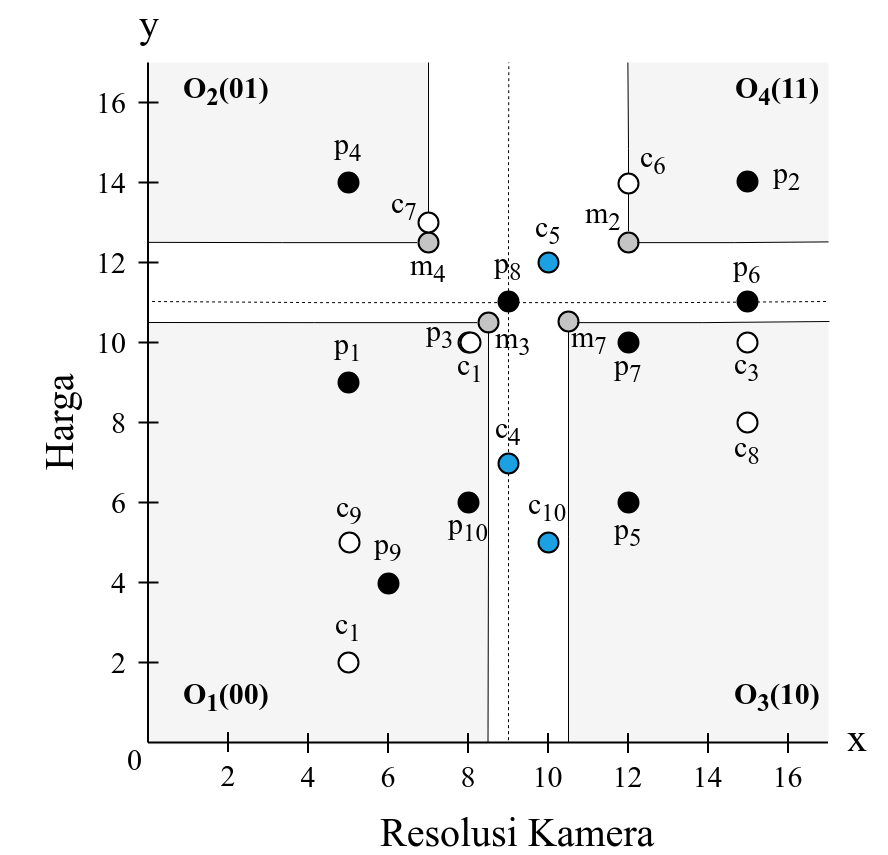
\includegraphics[height=6cm]{assets/img/bab2/rsl.png}
	\caption{Komputasi \textit{Reverse Skyline} dari Produk $p_8$}
	\label{fig:rsl}
\end{figure}

Sebagai contoh, berdasarkan \textit{dataset} yang diberikan pada Tabel \ref{tab:dataset}, \textit{reverse skyline} dari produk $p_8$ adalah pelanggan $c_4$, $c_5$, dan $c_{10}$, dinotasikan dengan $RSL(p_8) = \{c_4, c_5, c_{10}\}$ karena masing-masing pelanggan tersebut memiliki $p_8$ pada hasil \textit{dynamic skyline}-nya.

\section{Kueri \textit{k-Most Promising Products} ($k$-MPP)}
\tab Kueri \textit{k-Most Promising Products} ($k$-MPP) adalah sebuah strategi pemilihan produk yang dikenalkan oleh Islam dan Liu dalam penelitiannya \cite{kmpp}.

\subsection{\textit{Uniform Product Adoption} (UPA)}
\tab \textit{Uniform Product Adoption} (UPA) mengasumsikan bahwa semua produk $p \in P$ yang muncul pada hasil \textit{dynamic skyline} pelanggan $c \in C$ akan saling berkompetisi satu sama lain untuk menarik pelanggan $c$, sehingga produk-produk tersebut memiliki probabilitas yang sama untuk dibeli oleh pelanggan $c$.

Probabilitas produk $p$ dibeli oleh pelanggan $c$, dinotasikan dengan $Pr(c, p|P)$ dapat dijelaskan oleh persamaan berikut:
\begin{equation}\label{eq:probability}
Pr(c, p|P) = \left\{
				\begin{array}{ll}
					\frac{1}{|DSL(c)|} & \text{if } p \in DSL(c)\\
					0 & \text{otherwise}\\
				\end{array}
				\right.
\end{equation}

Berdasarkan Persamaan \ref{eq:probability}, dapat dipastikan bahwa setiap produk yang muncul dalam $DSL(c)$ memiliki kesempatan yang sama untuk dipilih oleh pelanggan $c$. Sebaliknya, produk yang tidak muncul dalam $DSL(c)$ tidak memiliki kesempatan sama sekali untuk dipilih oleh $c$.

Sebagai contoh menggunakan \textit{dataset} pada Tabel \ref{tab:dataset}, probabilitas produk $p_8$ dibeli oleh pelanggan $c_4$ adalah $Pr(c_4, p_8|P) = \frac{1}{|DSL(c_4)|} = \frac{1}{2}$, sedangkan probabilitas produk $p_8$ dibeli oleh pelanggan $c_{10}$ adalah $\frac{1}{|DSL(c_{10})|} = \frac{1}{3}$.

\subsubsection{\textit{Market Contribution}}
\tab \textit{Market contribution} atau kontribusi pasar sebuah produk $p \in P$ diukur dari total jumlah pelanggan yang mungkin lebih memilih membeli produk $p$ dibandingkan produk lain $p'$.

Asumsinya jika seorang pelanggan memiliki dua produk atau lebih dalam hasil \textit{dynamic skyline}-nya, maka ia akan memberikan bobot yang sama pada produk-produk tersebut sebagaimana yang sudah dijelaskan pada Persamaan \ref{eq:probability}. Sehingga, kontribusi pasar sebuah produk dihitung dari hasil akumulasi bobot yang didapatkan dari semua pelanggan $c \in C$.

Kontribusi pasar produk $p$, dinotasikan dengan $E(C, p|P)$, diperoleh dengan mengakumulasikan probabilitas produk dari setiap pelanggan $c \in C$, sebagai berikut:\\
\begin{equation}\label{eq:market-contr}
E(C, p|P) = \sum_{\forall c \in C} Pr(c, p|P)
\end{equation}

Karena probabilitas produk $p$ dipilih oleh pelanggan yang tidak memiliki $p$ pada hasil \textit{dynamic skyline}-nya adalah nol (pada Persamaan \ref{eq:probability}), maka kita hanya perlu mengakumulasikan probabilitas produk dari setiap pelanggan $c$ pada hasil $RSL(p)$. Sehingga, Persamaan \ref{eq:market-contr} dapat disederhanakan menjadi:
\begin{equation}\label{eq:market-contr-rsl}
E(C, p|P) = \sum_{\forall c \in RSL(p)} Pr(c, p|P)
\end{equation}

Sebagai contoh menggunakan \textit{dataset} pada Tabel \ref{tab:dataset}, kontribusi pasar dari produk $p_8$ adalah $E(C, p_8|P) = Pr(c_4, p_8|P) + Pr(c_5, p_8|P) + Pr(c_{10}, p_8|P) = \frac{1}{2} + 1 + \frac{1}{3} = \frac{11}{6}$ atau $1.833$.

Perhitungan kontribusi pasar juga dapat dilakukan pada sekumpulan produk atau \textit{subset} produk $P'$, dinotasikan dengan $E(C, P'|P)$, yang dijelaskan pada Persamaan \ref{eq:market-contr-subset}.
\begin{equation}\label{eq:market-contr-subset}
E(C, P'|P) = \sum_{\forall p \in P'} E(C, p|P)
\end{equation}

\subsection{Strategi Pemilihan Produk}
\tab Diberikan \textit{dataset} produk $P$, \textit{dataset} preferensi pelanggan $C$, dan bilangan bulat positif $k$ yang lebih kecil dari |P|. Kueri \textit{k-Most Promising Products} ($k$-MPP), dinotasikan oleh Persamaan \ref{eq:kmpp}, akan memilih \textit{subset} $k$ produk $P'$ dari $P$ yang memiliki kontribusi pasar lebih besar dibandingkan dengan \textit{subset} $k$ produk $P''$ dari $P$ yang lain \cite{kmpp}.
\begin{equation}\label{eq:kmpp}
k-MPP(P, C, k)
\end{equation}

Jika merangkum semua penjelasan di atas, langkah-langkah yang harus dilakukan untuk memproses kueri $k$-MPP adalah: (1) menghitung \textit{reverse skyline} dari setiap produk $p \in P$, (2) menghitung \textit{dynamic Skyline} dari setiap pelanggan $c \in RSL(p)$, dan (3) memilih \textit{k} produk dari $P$ yang memiliki kontribusi pasar terbesar.

\section{Python}
\tab Python adalah bahasa pemrograman tingkat tinggi, \textit{interpreted}, dan berorientasi objek yang didukung oleh struktur data \textit{built-in} tingkat tinggi dan semantik yang dinamis \cite{python}. Python dikembangkan oleh Guido van Rossum pada akhir 1980-an dan dikelola oleh \textit{Python Software Foundation}. Saat ini, Python sudah tersedia dalam dua versi, yakni 2.x dan 3.x.

Kelebihan bahasa pemrograman Python adalah pada keterbacaannya karena memiliki sintaksis yang sederhana, sehingga dapat mengurangi biaya pemeliharaan (\textit{maintenance}). Python mendukung banyak modul dan \textit{package}, serta memiliki banyak \textit{standard library} yang didistribusikan secara gratis. Selain itu, karena Python adalah bahasa \textit{interpreted}, Python tidak memakan biaya untuk kompilasi sehingga proses pengubahan, pengujian, dan debug menjadi lebih cepat.

Melakukan debug pada program Python sangatlah mudah karena tidak akan mengakibatkan \textit{segmentation fault}. Sebagai gantinya, ia akan menimbulkan \textit{Exception} apabila menemukan suatu \textit{error} atau kesalahan. Ketika program tidak menangkap \textit{Exception}, maka Python akan menampilkan \textit{stack trace} yang dapat digunakan untuk menganalisis dan memperbaiki kesalahan yang terjadi \cite{python}.

Pada Tugas Akhir ini, bahasa pemrograman Python digunakan untuk mengimplementasikan struktur data dan algoritme pada sistem perangkat lunak yang akan dibangun. 

\section{Flask}
\tab Flask adalah kerangka kerja web berbahasa Python yang sederhana, ringan, dan mudah dikembangkan, sehingga Flask kerap disebut dengan \textit{microframework}. Flask dibangun dari dua pustaka utama, yaitu Jinja \textit{template engine} dan Werkzeug WSGI \textit{toolkit}, serta memiliki lisensi BSD. Saat ini, Flask dikembangkan dan dikelola oleh \textit{Pallets team} dan kontributor komunitas.

Kerangka kerja Flask digunakan untuk mengimplementasikan aplikasi web dan layanan \textit{web server} yang digunakan pada Tugas Akhir ini karena ringan dan lebih mudah digunakan dibandingkan dengan \textit{framework} Python Django. Selain itu, Flask juga memiliki banyak dokumentasi dan tutorial yang dapat diikuti.

	\chapter{ANALISIS DAN PERANCANGAN SISTEM} \label{chapter:analisis dan perancangan sistem}
\tab Pada bab ini akan dijelaskan mengenai analisis dan perancangan sistem perangkat lunak yang akan dibangun, meliputi struktur data, algoritme, dan arsitektur aplikasi. 

\section{Daftar Notasi}
\tab Tabel \ref{tab:daftar-notasi-2} menunjukkan daftar notasi yang digunakan dalam bab ini beserta deskripsinya.

\begin{longtable}{| p{3cm} | p{7cm} |} 
	\caption{Daftar Notasi (2) \label{tab:daftar-notasi-2}}\\
	\hline
	\multicolumn{1}{|p{3cm}|}{\textbf{Notasi}} & \multicolumn{1}{|p{7cm}|}{\textbf{Deskripsi}}\\ \hline
	\hline
	\endfirsthead
	\hline
	\multicolumn{1}{|p{3cm}|}{\textbf{Notasi}} & \multicolumn{1}{|p{7cm}|}{\textbf{Deskripsi}}\\ \hline 
	\endhead
	$P$ & \textit{Dataset} produk\\ \hline
	$C$ & \textit{Dataset} pelanggan (preferensi pelanggan)\\ \hline
	$D$ & $P \cup C$ \\ \hline
	$ob$ & Sebuah objek data pada $D$\\ \hline
	$ob_1 \prec ob_2$ & Objek data $ob_1$ mendominasi $ob_2$\\ \hline
	$ob_1 \prec_{ob_3} ob_2$ & Objek data $ob_1$ mendominasi $ob_2$ berdasarkan $ob_3$\\ \hline
	$p$ & Sebuah produk dalam $P$, $p \in P$\\ \hline
	$c$ & Seorang pelanggan dalam $C$, $c \in C$\\ \hline
	$d$ & Jumlah dimensi pada $D$\\ \hline
	$i$ & Dimensi ke-1, ..., $d$\\ \hline
	$j$ & Timestamp ke-1, 2, ..., dst\\ \hline
	$O$ & \textit{Orthant} atau daerah pada komputasi \textit{reverse skyline}\\ \hline
	$m$ & \textit{Midpoint} antar produk pada komputasi \textit{reverse skyline}\\ \hline
	$DSL(c)$ & Hasil \textit{dynamic skyline} dari pelanggan $c$\\ \hline
	$RSL(p)$ & Hasil \textit{reverse skyline} dari produk $p$\\ \hline
	$Pr(c, p|P)$ & Probabilitas produk $p$ dibeli oleh pelanggan $c$ \\ \hline
	$E(C, p|P)$ & Kontribusi pasar $p$\\ \hline
	$E(C, P'|P)$ & Kontribusi pasar subset $P'$ dari $P$ \\ \hline
	$k-MPP$ & \textit{k-Most Promising Products} \\ \hline
	$k-MPPTI$ & \textit{k-Most Promising Products in Time Intervals} \\ \hline
\end{longtable}

\section{Analisis Sistem}
\tab Analisis sistem dijelaskan dalam empat bagian, yakni analisis permasalahan, deskripsi umum sistem, fungsi sistem, dan analisis kebutuhan fungsional.

\subsection{Analisis Permasalahan}
\tab Permalasahan yang ingin diselesaikan pada Tugas Akhir ini adalah bagaimana menjawab kueri \textit{$k$-Most Promising Products} berbasis interval waktu ($k$-MPPTI). Interval waktu, dinotasikan dengan $[t_i:t_e ](t_i \leq t_e)$, digunakan untuk menentukan rentang waktu pencarian. Sehingga, kueri $k$-MPP yang sudah ada \cite{kmpp} dimodifikasi menjadi:
\begin{equation}\label{eq:kmppts}
k-MPPTI(P, C, k, [t_i:t_e])
\end{equation} 

Permasalahan ini tidak dapat langsung diselesaikan menggunakan metode dan algoritme yang sudah ada \cite{kmpp}. Sehingga, diperlukan pendekatan lain yang akan dijelaskan pada bagian perancangan sistem.

\subsection{Deskripsi Umum Sistem}
\tab Secara umum, sistem yang akan dibangun adalah sebuah sistem berbasis web yang dapat membantu pengguna untuk memilih \textit{k}-produk yang paling menjanjikan. Dikatakan "menjanjikan" jika produk tersebut memiliki kontribusi pasar yang besar.

Sistem ini memiliki dua proses utama, yaitu (1) \textit{data precomputing} untuk menghitung kontribusi pasar masing-masing produk dan (2) proses utama (selanjutnya akan disebut dengan \textit{query processing}) untuk memproses dan menampilkan hasil kueri pencarian yang dimasukkan oleh pengguna.

Sistem ini dibangun menggunakan arsitektur \textit{client}-\textit{server}. Aplikasi \textit{client} didesain berbasis web dengan memanfaatkan Flask \textit{microframework}, HTML, CSS, dan JavaScript. Selain itu, Flask juga digunakan sebagai \textit{webserver}. 

\subsection{Fungsi Sistem}
\tab Sistem yang akan dibangun memiliki beberapa fungsi utama sebagai berikut:
\begin{enumerate}
	\item Dapat menerima \textit{input} data berupa file dari pengguna
	\item Dapat menampilkan informasi dan pratinjau data yang di-\textit{input}-kan oleh pengguna
	\item Dapat menampilkan visualisasi data
	\item Dapat melakukan proses \textit{data pre-computing} menggunakan algoritme yang dipilih oleh pengguna
	\item Dapat menerima \textit{input} kueri pencarian 
	\item Dapat memproses kueri pencarian
	\item Dapat menampilkan hasil kueri
	\item Dapat menampilkan waktu eksekusi
\end{enumerate}

\subsection{Analisis Kebutuhan Fungsional}
\tab Sistem yang dibuat harus mampu memenuhi beberapa fungsi utama yang telah dijelaskan pada sub-bagian sebelumnya. Fungsi-fungsi ini merupakan hasil dari analisis kebutuhan fungsional dari pengguna yang dijelaskan pada Tabel \ref{tab:kebutuhan-fungsional}.

\begin{table}[H]
	\small
	\centering
	\begin{tabular}{ | p{2cm} | p{6.5cm} | }
		\hline
		\textbf{Kode} & \textbf{Deskripsi Kebutuhan} \\ \hline \hline
		F-001 & Mengunggah data \\ \hline
		F-002 & Melihat informasi dan pratinjau data \\ \hline
		F-003 & Melihat visualisasi data  \\ \hline
		F-004 & Memilih algoritme yang digunakan untuk \textit{pre-processing}\\ \hline
		F-005 & Memasukkan kueri pencarian \\ \hline
		F-006 & Melihat hasil kueri \\ \hline
		F-007 & Melihat waktu eksekusi \\ \hline
	\end{tabular} \caption{Kebutuhan Fungsional}
	\label{tab:kebutuhan-fungsional}
\end{table}

Penjelasan rinci dari masing-masing kebutuhan fungsional pada tabel \ref{tab:kebutuhan-fungsional} dijelaskan sebagai berikut:
\begin{enumerate}
	\item \textbf{Mengunggah data}\\
	\tab Pengguna dapat mengunggah data produk dan preferensi pelanggan dalam bentuk file berekstensi csv.
	\item \textbf{Melihat informasi dan pratinjau data} \\
	\tab Pengguna dapat melihat informasi dan pratinjau dari data yang di-\textit{input}-kan berupa tabel sebanyak 20 baris. Informasi yang ditampilkan antara lain jumlah baris, jumlah kolom, dan nama kolom.
	\item \textbf{Melihat visualisasi data} \\
	\tab Pengguna juga dapat melihat visualisasi dari data yang di-\textit{input}-kan berupa \textit{timeline} sederhana.
	\item \textbf{Memilih algoritme yang digunakan untuk \textit{pre-processing}} \\
	\tab Pengguna dapat memilih algoritme yang akan digunakan untuk \textit{data pre-processing}, yaitu algoritme $k$-MPPTI dan Brute Force.
	\item \textbf{Mamasukkan kueri pencarian} \\
	\tab Pengguna dapat memasukkan kueri pencarian berupa jumlah produk ($k$) dan interval waktu.
	\item \textbf{Melihat hasil kueri} \\
	\tab Pengguna dapat melihat hasil kueri pencarian berupa $k$-produk dengan jumlah kontribusi pasar terbesar beserta skor kontribusi pasar-nya. 
	\item \textbf{Melihat waktu eksekusi} \\
	\tab Pengguna dapat melihat informasi terkait waktu eksekusi.
\end{enumerate}

\section{Perancangan Sistem}
\tab Perancangan sistem akan dibagi menjadi empat bagian, yakni struktur data, algoritme utama, algoritme pembanding menggunakan metode \textit{brute force}, dan arsitektur aplikasi. 

\subsection{Struktur Data}
\tab Struktur data adalah suatu cara untuk menyimpan, menyusun, mengelompokkan, dan merepresentasikan suatu data. Ada tiga struktur data utama yang digunakan dalam komputasi $k$-MPPTI, yaitu untuk menyimpan data produk dan pelanggan, \textit{Event Queue}, dan \textit{Pandora Box}.

\subsubsection{Data Produk dan Pelanggan}

Data yang diolah dalam Tugas Akhir ini adalah data produk dan pelanggan yang disimpan dalam struktur data \textit{nested dictionary}. Struktur data ini efisien untuk pencarian data karena menggunakan konsep \textit{key-value pairs}, berbeda dengan struktur data \textit{list} atau \textit{array} yang menggunakan indeks untuk mengakses nilai suatu data.

Struktur data \textit{dictionary} yang digunakan terdiri dari dua \textit{key} utama, yaitu '$product$' yang menyimpan data produk dan '$customer$' yang menyimpan data preferensi pelanggan. Struktur \textit{nested key} masing-masing data dijelaskan pada Gambar \ref{fig:sd1} dan \ref{fig:sd2}.

\begin{figure}[h]
	\centering
	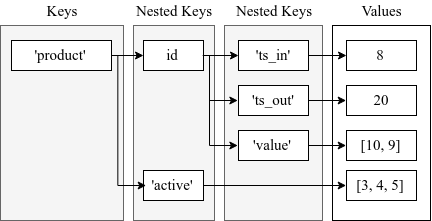
\includegraphics[width=6cm]{bab3/img/sd1.png}
	\caption{Struktur Data \textit{Dictionary} Produk}
	\label{fig:sd1}
\end{figure}

Pada struktur data produk, nilai $id$ digunakan sebagai \textit{key}.  

\begin{figure}[h]
	\centering
	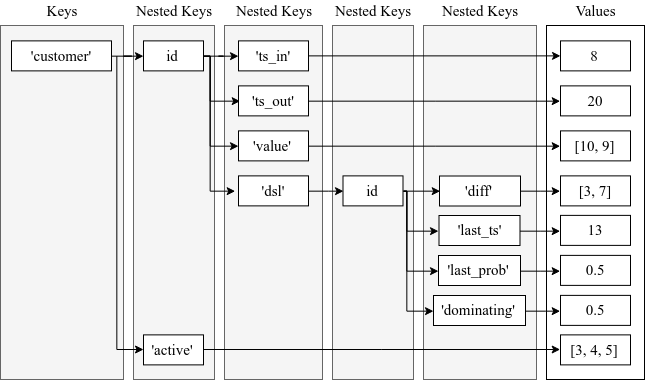
\includegraphics[width=9cm]{bab3/img/sd2.png}
	\caption{Struktur Data \textit{Dictionary} Pelanggan}
	\label{fig:sd2}
\end{figure}

 

\begin{table}[H]
	\centering
	\begin{tabular}{ | p{1.5cm} | p{7.5cm} | }
		\hline
		\textbf{Key} & \textbf{Value} \\ \hline \hline
		$id$ & ID unik data \\ \hline
		$ts\_in$ & \textit{Timestamp} masuk \\ \hline
		$ts\_out$ & \textit{Timestamp} keluar \\ \hline
		$value$ & Nilai data pada semua atribut/dimensi yang disimpan dalam bentuk \textit{array}\\ \hline
		$dsl$ & Hasil \textit{dynamic skyline} yang disimpan dalam bentuk \textit{dictionary} \\ \hline
		$diff$ & Selisih antara nilai atribut
	\end{tabular} 
	\caption{Deskripsi \textit{Key} dan \textit{Value}}
	\label{tab:desc-key}
\end{table}

\subsubsection{\textit{Event Queue}}

\subsubsection{\textit{Pandora Box}}
\tab \textit{Pandora Box} adalah sebuah struktur data array dua dimensi, sumbu $x$ adalah \textit{timestamp} dan sumbu $y$ adalah produk. Struktur data ini digunakan untuk menyimpan skor kontribusi pasar setiap waktu. Menggunakan contoh \textit{dataset} pada Tabel \ref{tab:dataset-2}, \textit{Pandora Box} yang dibutuhkan seperti di bawah ini.  



\subsection{Algoritme Utama}
\tab Sebagaimana yang telah dijelaskan sebelumnya bahwa algoritme utama terdiri dari dua tahap pemrosesan, yaitu \textit{data precomputing} dan \textit{query processing}. Secara garis besar, alur kerja sistem secara umum disajikan dalam bentuk diagram alur yang dapat dilihat pada Gambar ...

Tahap \textit{data precomputing} bertujuan untuk menghitung kontribusi pasar masing-masing produk berdasarkan preferensi pelanggan. Diawali dengan pembentukan \textit{Event Queue} untuk mencatat semua \textit{event} yang terjadi selama pemrosesan data. Kemudian, memproses \textit{event-event} tersebut menggunakan algoritme pemrosesan berdasarkan jenis \textit{event}-nya. Terakhir adalah menghitung kontribusi pasar dan menyimpannya ke dalam struktur data \textit{array} bernama \textit{Pandora Box}.

\textit{Pandora Box} kemudian digunakan sebagai \textit{input} pada tahap \textit{query processing}. Diawali dengan \textit{input} kueri pencarian berupa jumlah produk ($k$) dan interval waktu pencarian. Kemudian, mencari produk sejumlah $k$ yang memiliki total skor kontribusi pasar terbesar selama interval waktu pencarian. Terakhir adalah mengembalikan hasil kueri pencarian berupa $k$-produk yang paling menjanjikan kepada pengguna.

Untuk memudahkan interaksi antara pengguna dan sistem, dibuatlah aplikasi berbasis \textit{web} yang memudahkan pengguna meng-\textit{input}-kan data produk dan pelanggan, melihat pratinjau dan visualisasi data, meng-\textit{input}-kan kueri pencarian, serta melihat hasil kueri pencarian.   

\subsubsection{\textit{Data Precomputing}}
\tab \textit{Data precomputing} adalah sebuah proses yang dapat menunjang performa algoritme \textit{query processing} supaya dapat bekerja lebih efektif dan efisien. Tidak adanya proses \textit{data precomputing} menyebabkan pengulangan komputasi data setiap kali seseorang memasukkan kueri pencarian, sehingga komputasi data cukup dilakukan satu kali di awal (\textit{precomputing}). Berbeda halnya jika data yang digunakan adalah data \textit{streaming} yang nilainya terus berubah dalam periode waktu tertentu.
	
\newcolumntype{C}{>{\centering\arraybackslash}p{1.4em}}
\begin{table}[H]
	\caption{Contoh \textit{Dataset} \\ (a) Produk $P$ dan (b) Preferensi Pelanggan $C$ \label{tab:dataset-2}}
	\begin{subtable}{.5\linewidth}
		\small
		\centering
		\caption{}
		\begin{tabular}{|C|C|C|C|C|}
			\hline
			\multirow{2}{*}{\textbf{ID}} & \multicolumn{2}{c|}{\textbf{\textit{Timestamp}}} & \multicolumn{2}{c|}{\textbf{Nilai}} \\ \cline{2-5}
			& \textbf{$t_i$} & \textbf{$t_e$} & \textbf{$d_1$} & \textbf{$d_2$}\\ \hline \hline
			$p_1$ & 2 & 10 & 6 & 3 \\ \hline
			$p_2$ & 6 & 13 & 4 & 12 \\ \hline
			$p_3$ & 9 & 15 & 6 & 15 \\ \hline
			$p_4$ & 4 & 9 & 9 & 5 \\ \hline
			$p_5$ & 5 & 15 & 12 & 10 \\ \hline
		\end{tabular}
	\end{subtable}%
	\begin{subtable}{.5\linewidth}
		\small
		\centering
		\caption{}
		\begin{tabular}{|C|C|C|C|C|}
			\hline
			\multirow{2}{*}{\textbf{ID}} & \multicolumn{2}{c|}{\textbf{\textit{Timestamp}}} & \multicolumn{2}{c|}{\textbf{Nilai}} \\ \cline{2-5}
			 & \textbf{$t_i$} & \textbf{$t_e$} & \textbf{$d_1$} & \textbf{$d_2$}\\ \hline \hline
			$c_1$ & 1 & 8 & 2 & 8 \\ \hline
			$c_2$ & 4 & 14 & 4 & 10\\ \hline
			$c_3$ & 10 & 15 & 6 & 11\\ \hline
			$c_4$ & 3 & 8 & 8 & 12\\ \hline
			$c_5$ & 5 & 15 & 9 & 10\\ \hline
		\end{tabular}
	\end{subtable} 
\end{table}

Untuk memudahkan penjelasan algoritme, pada Tabel \ref{tab:dataset-2}, diberikan contoh \textit{dataset} produk $P$ dan preferensi pelanggan $C$ yang setiap datanya direpresentasikan sebagai titik $d$-dimensi dengan serial waktu $[t_i:t_e]$. Data dimodelkan sebagai \textit{timeline} yang diilustrasikan pada Gambar .... Setiap ada data $d \in D$ yang masuk atau keluar akan dicatat sebagai \textit{event} $e \in E$ dan dimasukkan ke dalam struktur data \textit{queue} bernama \textit{Event Queue}. Contoh \textit{Event Queue} yang terbentuk dari \textit{dataset} pada Tabel \ref{tab:dataset-2} ditunjukkan pada Tabel \ref{tab:event-queue}.

\begin{small}
	\begin{longtable}{|c|c|c|c|}
		\caption{Event Queue \label{tab:event-queue}}
		\hline
		\multicolumn{1}{|c|}{\textbf{ID \textit{Event}}} & \multicolumn{1}{c|}{\textbf{\textit{Timestamp}}} & \multicolumn{1}{c}{\textbf{ID Data}} & \multicolumn{1}{|c|}{\textbf{Aksi}} \\ \hline 
		\endfirsthead
		\hline
		\multicolumn{1}{|c|}{\textbf{ID \textit{Event}}} & \multicolumn{1}{c|}{\textbf{\textit{Timestamp}}} & \multicolumn{1}{c}{\textbf{ID Data}} & \multicolumn{1}{|c|}{\textbf{Aksi}} \\ \hline
		\endhead
		$e_1$ & 1 & $c_1$ & Masuk \\ \hline
		$e_2$ & 2 & $p_1$ & Masuk \\ \hline
		$e_3$ & 3 & $c_4$ & Masuk \\ \hline
		$e_4$ & 4 & $p_4$ & Masuk \\ \hline
		$e_5$ & 4 & $c_2$ & Masuk \\ \hline
		$e_6$ & 5 & $p_5$ & Masuk \\ \hline
		$e_7$ & 5 & $c_5$ & Masuk \\ \hline
		$e_8$ & 6 & $p_2$ & Masuk \\ \hline
		$e_9$ & 8 & $c_1$ & Keluar \\ \hline
		$e_{10}$ & 8 & $c_4$ & Keluar \\ \hline
		$e_{11}$ & 9 & $p_3$ & Masuk \\ \hline
		$e_{12}$ & 9 & $p_4$ & Keluar \\ \hline
		$e_{13}$ & 10 & $c_3$ & Masuk \\ \hline
		$e_{14}$ & 10 & $p_1$ & Keluar \\ \hline
		$e_{15}$ & 13 & $p_2$ & Keluar \\ \hline
		$e_{16}$ & 14 & $c_2$ & Keluar \\ \hline
		$e_{17}$ & 15 & $p_3$ & Keluar \\ \hline
		$e_{18}$ & 15 & $p_5$ & Keluar \\ \hline
		$e_{19}$ & 15 & $c_3$ & Keluar \\ \hline
		$e_{20}$ & 15 & $c_5$ & Keluar \\ \hline
	\end{longtable}
\end{small}

Kemudian, \textit{event-event} ini akan diproses secara berurutan menggunakan algoritme yang sesuai dengan jenis \textit{event}-nya. Ada empat jenis proses yang dilakukan berdasarkan jenis \textit{event}, yaitu: (1) produk masuk (\textit{product insertion}), (2) produk keluar (\textit{product deletion}), (3) pelanggan masuk (\textit{customer insertion}), dan (4) pelanggan keluar (\textit{customer deletion}). 

Terlepas dari empat jenis pemrosesan \textit{event}, sebenarnya hanya ada dua jenis komputasi \textit{skyline} yang digunakan dalam \textit{data precomputing}, yaitu \textit{dynamic skyline} dan \textit{reverse skyline}. Dua komputasi tersebut digunakan sebagai metode perhitungan probabilitas dan kontribusi pasar. 

\myparagraph{Komputasi \textit{Dynamic Skyline}}

Sebagaimana yang telah dijelaskan pada Bab Tinjauan Pustaka, komputasi \textit{dynamic skyline} digunakan untuk mencari produk terbaik dari sudut pandang pelanggan \cite{kmpp}. \textit{Dynamic skyline} \cite{dynamic-skyline} dari seorang pelanggan $c_1 \in C$, dinotasikan dengan $DSL(c_1)$, berisi semua produk $p_1 \in P$ yang tidak didominasi oleh produk lain $p_2 \in P$ berdasarkan preferensi pelanggan $c_1$, $p_2 \nprec_{c_1} p_1$. 

Proses komputasi \textit{dynamic skyline} diawali dengan perhitungan selisih absolut dari nilai masing-masing dimensi antara pelanggan dan produk, dinotasikan dengan:
\begin{equation}\label{eq:diff}
diff^i = |c_1^i - p^i|
\end{equation}

Selanjutnya, mengecek dominansi dinamis antar produk dengan membandingkan selisih absolut-nya. Misalnya, ada dua produk yang akan dibandingkan, dinotasikan dengan $p_s$ sebagai subjek yang dibandingkan dan $p_o$ sebagai objek pembanding. Berdasarkan syarat dominansi dinamis (Persamaan \ref{eq:syarat-dominansi-dinamis}), $p_s$ dikatakan mendominasi $p_o$ jika dan hanya jika:
\begin{equation}\label{eq:komputasi-dsl}
\begin{split}
\text{(a)} \tab diff_s^i \leq diff_o^i, \forall i \in [1, ..., d] \\
\text{(b)} \tab diff_s^i < diff_o^i, \exists i \in [1, ..., d]
\end{split}
\end{equation}

Pengecekan dominansi dinamis ini dilakukan secara iteratif sampai dipastikan suatu $p_1$ tidak didominasi oleh $p_2$ lain sama sekali. Jika $p_1$ pernah didominasi, maka $p_1$ tidak dapat menjadi hasil \textit{dynamic skyline}.

Menggunakan contoh \textit{dataset} pada Tabel \ref{tab:dataset-2}, dengan mengabaikan \textit{timestamp}-nya akan didapatkan perhitungan hasil \textit{dynamic skyline} seperti pada Tabel \ref{tab:dsl-res}.

\begin{table}[H]
	\small
	\centering
	\begin{tabular}{|p{2cm}|p{3cm}|}
		\hline
		$DSL(c_1)$ & $\{2, 4, 5\}$ \\ \hline
		$DSL(c_2)$ & $\{2, 5\}$ \\ \hline
		$DSL(c_3)$ & $\{2, 3\}$ \\ \hline
		$DSL(c_4)$ & $\{2, 3, 4\}$\\ \hline
		$DSL(c_5)$ & $\{4, 5\}$ \\ \hline
	\end{tabular} 
	\caption{Hasil Perhitungan \textit{Dynamic Skyline} dari \textit{Dataset} \ref{tab:dataset-2}}
	\label{tab:dsl-res}
\end{table}


\myparagraph{Komputasi \textit{Reverse Skyline}}

Komputasi \textit{reverse skyline} digunakan untuk mencari pelanggan potensial dari sudut pandang produsen \cite{kmpp}. \textit{Reverse skyline} \cite{reverse-skyline} dari sebuah produk $p_1 \in
P$, dinotasikan dengan $RSL(p_1)$, berisi semua pelanggan $c \in C$ yang memiliki $p_1$ pada hasil \textit{dynamic skyline}-nya.

Sebagaimana yang telah dijelaskan pada Tinjauan Pustaka, komputasi \textit{reverse skyline} diawali dengan menentukan \textit{orthant} dari produk, dinotasikan dengan $O$. Dalam geometri, \textit{orthant} adalah analog dalam ruang data \textit{d}-dimensi atau biasa dikenal sebagai kuadran dalam bidang dua dimensi. Setiap produk $p$ memiliki $2^d$ \textit{orthant} pada data $d-$dimensi. 

\textit{Orthant} ditandai menggunakan bilangan biner. Sebagai contoh, terdapat empat \textit{orthant} pada bidang dua dimensi, yaitu $O_{00}$, $O_{01}$, $O_{10}$, dan $O_{11}$, dan delapan \textit{orthant} pada bidang tiga dimensi, yaitu $O_{000}$, $O_{001}$, $O_{010}$, $O_{011}$, $O_{100}$, $O_{101}$, $O_{110}$ dan $O_{111}$. Penggunaan bilangan biner bertujuan untuk menandai batas wilayah sebuah \textit{orthant}. Misalnya, \textit{orthant} $O_{010}$ dari produk $p_1$ memiliki wilayah dengan batas-batas sebagai berikut: sumbu $x$ (0 - $pos_x(p_1)$), sumbu $y$ ($pos_y(p_1)$ - $max_y$), dan sumbu $z$ (0 - $pos_z(p_1)$).

Langkah selanjutnya adalah menghitung \textit{midpoint} atau titik tengah antara produk kueri dan produk lainnya, misalnya $p_1$ (sebagai titik kueri) dan $p_2 \in P$, menggunakan rumus berikut: 
\begin{equation} \label{eq:midpoint2}
m_2^i = \frac{(p_1^i + p_2^i)}{2}
\end{equation}
Kemudian, menentukan \textit{midpoint skyline} atau \textit{mid-skyline} \cite{mid-skyline} pada setiap \textit{orthant}.

Langkah terakhir adalah mengecek setiap pelanggan $c \in C$ apakah didominasi oleh hasil \textit{mid-skyline} pada masing-masing \textit{orthant} atau tidak (Persamaan \ref{eq:mid-skyline}). Jika $c$ didominasi, maka $c$ tidak dapat menjadi hasil \textit{reverse skyline}.

\myparagraph{Perhitungan Probabilitas}

Setelah mendapatkan hasil \textit{dynamic skyline} pada Tabel \ref{tab:dsl-res}, selanjutnya adalah menghitung probabilitas masing-masing produk $p$ dipilih oleh pelanggan $c$, dinotasikan dengan $Pr(c, p|P)$, yang telah dijelaskan pada Persamaan \ref{eq:probability}. Sehingga, dari Tabel \ref{tab:dsl-res} akan didapatkan hasil perhitungan probabilitas sebagai berikut.

\begin{small}
	\begin{longtable}{|p{1.5cm}|p{3cm}|p{2.5cm}|}
		\caption{Hasil Perhitungan Probabilitas dari Tabel \ref{tab:dsl-res}}
		\label{tab:prob-res}
		\hline
		\multirow{5}{*}{$p_1$} & $Pr(c_1, p_1|P)$ & $0$ \\ \cline{2-3}
		& $Pr(c_2, p_1|P)$ & $0$ \\ \cline{2-3}
		& $Pr(c_3, p_1|P)$ & $0$ \\ \cline{2-3}
		& $Pr(c_4, p_1|P)$ & $0$ \\ \cline{2-3}
		& $Pr(c_5, p_1|P)$ & $0$ \\ \hline
		\multirow{5}{*}{$p_2$} & $Pr(c_1, p_2|P)$ & $\frac{1}{3} = 0.33$ \\ \cline{2-3}
		& $Pr(c_2, p_2|P)$ & $\frac{1}{2} = 0.5$ \\ \cline{2-3}
		& $Pr(c_3, p_2|P)$ & $\frac{1}{2} = 0.5$ \\ \cline{2-3}
		& $Pr(c_4, p_2|P)$ & $\frac{1}{3} = 0.33$  \\ \cline{2-3}
		& $Pr(c_5, p_2|P)$ & $0$ \\ \hline
		\multirow{5}{*}{$p_3$} & $Pr(c_1, p_3|P)$ & $0$ \\ \cline{2-3}
		& $Pr(c_2, p_3|P)$ & $0$ \\ \cline{2-3}
		& $Pr(c_3, p_3|P)$ & $\frac{1}{2} = 0.5$ \\ \cline{2-3}
		& $Pr(c_4, p_3|P)$ & $\frac{1}{3} = 0.33$  \\ \cline{2-3}
		& $Pr(c_5, p_3|P)$ & $0$ \\ \hline
		\multirow{5}{*}{$p_4$} & $Pr(c_1, p_4|P)$ & $\frac{1}{3} = 0.33$ \\ \cline{2-3}
		& $Pr(c_2, p_4|P)$ & $0$ \\ \cline{2-3}
		& $Pr(c_3, p_4|P)$ & $0$ \\ \cline{2-3}
		& $Pr(c_4, p_4|P)$ & $\frac{1}{3} = 0.33$  \\ \cline{2-3}
		& $Pr(c_5, p_4|P)$ & $\frac{1}{2} = 0.5$ \\ \hline
		\multirow{5}{*}{$p_5$} & $Pr(c_1, p_5|P)$ & $\frac{1}{3} = 0.33$ \\ \cline{2-3}
		& $Pr(c_2, p_5|P)$ & $\frac{1}{2} = 0.5$ \\ \cline{2-3}
		& $Pr(c_3, p_5|P)$ & $0$ \\ \cline{2-3}
		& $Pr(c_4, p_5|P)$ & $0$  \\ \cline{2-3}
		& $Pr(c_5, p_5|P)$ & $\frac{1}{2} = 0.5$ \\ \hline
	\end{longtable}
\end{small}

\myparagraph{Perhitungan Kontribusi Pasar (\textit{Market Contribution})}

Hasil perhitungan probabilitas produk $p$ pada Tabel \ref{tab:prob-res} kemudian diakumulasikan menjadi skor kontribusi pasar sebagaimana yang dijelaskan pada Persamaan \ref{eq:market-contr}. Sehingga akan didapatkan hasil pada Tabel \ref{tab:mc-res}.

\begin{table}[H]
	\small
	\centering
	\begin{tabular}{|p{3cm}|p{2cm}|}
		\hline
		$E(C, p_1|P)$ & $0$ \\ \hline
		$E(C, p_2|P)$ & $1.66$ \\ \hline
		$E(C, p_3|P)$ & $0.83$ \\ \hline
		$E(C, p_4|P)$ & $1.16$ \\ \hline
		$E(C, p_5|P)$ & $1.33$ \\ \hline
	\end{tabular} 
	\caption{Hasil Perhitungan Kontribusi Pasar dari Tabel \ref{tab:prob-res}}
	\label{tab:mc-res}
\end{table}

\myparagraph{Proses \textit{Product Insertion}}

Proses \textit{Product Insertion} adalah proses yang dijalankan ketika ada produk yang masuk ke dalam \textit{timeline}. Ketika ada data produk yang masuk, ada kemungkinan jika produk tersebut menjadi hasil \textit{dynamic skyline} suatu pelanggan $c \in C$ sehingga mengubah hasil perhitungan probabilitasnya. Hasil dari proses ini adalah \textit{Pandora Box} yang telah diperbarui.

Algoritme pemrosesan yang dilakukan adalah:
\begin{enumerate}
	\item Menambah produk $p$ ke dalam daftar produk aktif, dinotasikan dengan $P_a$
	\item Menghitung $RSL(p)$
	\item Menghitung $DSL(c), \forall c \in RSL(p)$ 
	\item Memperbarui \textit{Pandora Box}
\end{enumerate}

\myparagraph{Proses \textit{Product Deletion}}

Proses \textit{Product Deletion} adalah proses yang dijalankan ketika ada produk yang keluar dari \textit{timeline}. Produk yang keluar dinotasikan dengan $p_{out}$. Ketika ada data produk yang keluar, ada kemungkinan jika produk tersebut menjadi hasil \textit{dynamic skyline} suatu pelanggan $c \in C$ sehingga mengubah hasil perhitungan probabilitasnya. Sama seperti proses \textit{product insertion}, hasil dari proses ini adalah \textit{Pandora Box} yang telah diperbarui.

Algoritme pemrosesan yang dilakukan adalah:
\begin{enumerate}
	\item Memperbarui \textit{Pandora Box}
	\item Menghitung $RSL(p_{out})$
	\item Menghitung $DSL(c), \forall c \in RSL(p_{out})$
	\item Menghapus produk $p$ ke dalam daftar produk aktif, dinotasikan dengan $P_a$
\end{enumerate}

\myparagraph{Proses \textit{Customer Insertion}}

Proses \textit{Customer Insertion} adalah proses yang dijalankan ketika ada pelanggan yang masuk ke dalam \textit{timeline}. 

Algoritme pemrosesan yang dilakukan adalah:
\begin{enumerate}
	\item Menambah pelanggan $c$ ke dalam daftar pelanggan aktif, dinotasikan dengan $C_a$
	\item Menghitung \textit{Initial} $DSL(c)$ 
	\item Memperbarui \textit{Pandora Box}
\end{enumerate}

\myparagraph{Proses \textit{Customer Deletion}}

Proses \textit{Customer Deletion} adalah proses yang dijalankan ketika ada pelanggan yang keluar dari \textit{timeline}. 

Algoritme pemrosesan yang dilakukan adalah:
\begin{enumerate}
	\item Memperbarui \textit{Pandora Box}
	\item Menghapus pelanggan $c$ dari daftar pelanggan aktif $C_a$
\end{enumerate}

\subsubsection{\textit{Query Processing}}

\subsection{Algoritme \textit{Brute Force}}

\subsection{Arsitektur Aplikasi} 
\tab Sistem akan diimplementasikan menggunakan arsitektur \textit{client}-\textit{server} dan antarmuka pengguna grafis berbasis situs web, sebagaimana yang diilustrasikan pada Gambar ... Terdapat dua komponen utama dalam arsitektur ini, yakni:

\begin{enumerate}
	\item Client
	
	\tab Menampilkan antarmuka pengguna grafis berbasis situs web. 
\end{enumerate}
	\chapter{IMPLEMENTASI}
\label{chapter:implementasi}

Pada bab ini dijelaskan mengenai implementasi dari desain dan algoritma penyelesaian \problem{}.

\section{Lingkungan Implementasi}
Lingkungan implementasi dalam pembuatan Tugas Akhir ini meliputi perangkat keras dan perangkat lunak yang digunakan untuk penyelesaian \problem{} adalah sebagai berikut:

\begin{enumerate}
	\item Perangkat Keras:
		\begin{itemize}
			\item \textit{Processor} Intel(R) Core(TM) i3 - M 330 CPU @ 2.13GHz x 4 \item Memori 4 GB.
		\end{itemize}
	\item Perangkat Lunak:
	\begin{itemize}
		\item Sistem operasi Ubuntu 14.04 LTS 64 bit.
		\item \textit{Text editor} Sublime Text 3.
		\item \textit{Compiler} g++ versi 4.3.2.
	\end{itemize}			
\end{enumerate}


\section{Rancangan Data}
Pada subbab ini dijelaskan mengenai desain data masukan yang diperlukan untuk melakukan proses algoritma, dan data keluaran yang dihasilkan oleh program.

\subsection{Data Masukan}
Data masukan adalah data yang akan diproses oleh program sebagai masukan menggunakan algoritma dan struktur data yang telah dirancang dalam Tugas Akhir ini.\\
Data masukan berupa berkas teks yang berisi data dengan format yang telah ditentukan pada deskripsi \problem{}. Pada masing-masing berkas data masukan, baris pertama berupa sebuah bilangan bulat yang merepresentasikan jumlah kasus uji yang ada pada berkas tersebut. Untuk setiap kasus uji dengan tipe $1$ dan $2$, masukan berupa sebuah baris masukan yang terdiri dari dua buah parameter posisi berupa $x$ dan $y$. Sedangkan pada kasus uji dengan tipe $3$, masukan berupa sebuah parameter $y$ yang merupakan indeks \textit{string} yang dicari pada konfigurasi \textit{rope} saat ini.

\subsection{Data Keluaran}
Data keluaran yang dihasilkan oleh program hanya berupa satu nilai, yaitu huruf pada indeks ke-$y$ untuk setiap kasus uji dengan tipe $3$. 

\section{Implementasi Algoritma}
Pada subbab ini akan dijelaskan tentang implementasi proses algoritma secara keseluruhan berdasarkan desain yang telah dijelaskan pada Bab \ref{chapter:desain}.

\subsection{\textit{Header} yang Diperlukan}
Implementasi algoritma dengan pemanfaatan struktur data Rope untuk menyelesaikan \problem{} membutuhkan empat buah \textit{header} yaitu stdio.h, cstdlib, cstring dan utility, seperti yang terlihat pada Kode Sumber \ref{source:header}.\\

\lstinputlisting[language=C++, firstline=1, lastline=4, caption=\textit{Header} yang diperlukan, label=source:header]{assets/code/include.cpp}

\textit{Header} stdio.h berisi modul untuk menerima masukan dan memberikan keluaran. \textit{Header} cstdlib berisi modul untuk manajemen memori dinamis, generasi bilangan acak, pemilahan dan konversi. \textit{Header} cstring berisi modul yang memiliki fungsi-fungsi untuk melakukan pemrosesan \textit{string}. \textit{Header} utility mencakup berbagai modul yang menyediakan fungsionalitas mulai dari aplikasi perhitungan bit hingga aplikasi fungsi parsial. Contoh implementasinya penggunaan \textit{pair}. 

\subsection{Variabel Global}
Variabel global digunakan untuk memudahkan dalam mengakses data yang digunakan lintas fungsi. Kode sumber implementasi variabel global dapat dilihat pada Kode Sumber \ref{source:variabel_global}.

\begin{minipage}{\linewidth}
\lstinputlisting[language=C++, firstline=1, lastline=3, caption=Variabel Global, label=source:variabel_global]{assets/code/global.cpp}
\end{minipage}
	
\subsection{Implementasi Fungsi Main}
Fungsi Main adalah implementasi algoritma yang dirancang pada Gambar \ref{figure:fungsi_main}. Setiap tipe memiliki operasi yang berbeda-beda. Untuk operasi dengan tipe $3$, masukan hanya berupa parameter $y$ yang merupakan nilai posisi indeks yang dicari pada konfigurasi \textit{rope} saat ini. Pada operasi dengan tipe $1$ dan $2$, baris masukan berupa nilai $x$ dan $y$ yang merupakan posisi indeks dari \textit{string} pada \textit{rope}. Setiap masukan dengan tipe $3$ akan ditampilkan sebagai jawaban akhir dari permasalahan. Implementasi fungsi Main dapat dilihat pada Kode Sumber \ref{source:fungsi_main}.

\lstinputlisting[language=C++, firstline=1, lastline=24, caption=Fungsi Main, label=source:fungsi_main]{assets/code/main.cpp}

\subsection{Implementasi Struct Node}
Fungsi Struct Node berisi atribut yang dimiliki \textit{node} pada \textit{tree}. Implementasi dari fungsi Struct Node dapat dilihat pada Kode Sumber \ref{source:fungsi_struct}.

\lstinputlisting[language=C++, firstline=1, lastline=17, caption=Fungsi Struct Node, label=source:fungsi_struct]{assets/code/struct.cpp}

\subsection{Implementasi Fungsi Newnode}
Fungsi Newnode digunakan untuk membentuk sebuah \textit{node} yang berisikan karakter yang diberikan dan relasi terhadap karakter pada posisi yang bersebelahan. Sehingga membentuk sebuah \textit{tree} seperti pada Gambar \ref{fig:bst}. Implementasi fungsi \proc{newnode} dapat dilihat pada Kode Sumber \ref{source:fungsi_newnode}.

\lstinputlisting[language=C++, firstline=1, lastline=7, caption=Fungsi Newnode, label=source:fungsi_newnode]{assets/code/newnode.cpp}

\subsection{Implementasi Fungsi Build}
Fungsi Build membangun struktur \textit{tree} dari \textit{rope} yang dilakukan dari karakter yang berada pada posisi indeks di tengah sampai pada karakter paling awal maupun akhir.  Setiap \textit{node} akan memiliki anak kiri dan anak kanan jika dan hanya jika masih terdapat \textit{string} yang tersisa. Ilustrasinya dapat dilihat pada Gambar \ref{fig:rope}. Implementasi dari Fungsi Build dapat dilihat pada Kode Sumber \ref{source:fungsi_build}.

\lstinputlisting[language=C++, firstline=1, lastline=6, caption=Fungsi Build, label=source:fungsi_build]{assets/code/build.cpp}

\subsection{Implementasi Fungsi Getsize}
Fungsi Getsize digunakan untuk mendapatkan berat \textit{node} yang diperlukan. Implementasi dari fungsi Getsize dapat dilihat pada Kode Sumber \ref{source:fungsi_getsize}.

\lstinputlisting[language=C++, firstline=1, lastline=3, caption=Fungsi Getsize, label=source:fungsi_getsize]{assets/code/getsize.cpp}

\subsection{Implementasi Fungsi Split}
Fungsi Split memanfaatkan struktur data Pair yang berupa pasangan dari dua \textit{pointer} menuju \textit{node}. \textit{Pointer node} pertama akan berisi semua \textit{node} yang bernilai lebih kecil dari posisi indeks parameter \textit{split}, sedangkan \textit{pointer node} kedua berisi semua \textit{node} yang bernilai lebih besar sama dengan posisi indeks parameter \textit{split}.\\
Misalkan dilakukan \textit{split} pada indeks ke-$5$ dari \textit{rope} pada Gambar \ref{fig:split-5}, \textit{pointer node} pertama akan menyimpan semua \textit{node} dari indeks ke-$0$ sampai dengan $4$. Sedangkan \textit{pointer node} kedua menyimpan \textit{node} dari indeks ke-$5$ sampai akhir. Implementasi dari fungsi \textit{split} dapat dilihat pada Kode Sumber \ref{source:fungsi_split1} dan \ref{source:fungsi_split2}.
\begin{figure}
\centering
\begin{tikzpicture}[level/.style={sibling distance = 8cm/#1, level distance = 1.5cm}, scale=0.6,transform shape]
\node[treenode]{b,12}
  child{
    node[treenode]{t,6} 
    child {
    	node[treenode] {a,3}
    	child {
    		node[treenode]{g,1}
    	}
    	child{
    		node[treenode] {u,1}
    	}
    }
    child {
    	node[treenode] {m,2}
    	child {
    	    node[treenode] {a,1}
    	}
    	child[missing]{}
    }
  }
  child{
  	node[treenode]{h,5}
  	child {
  	    	node[treenode] {s,2}
  	    	child {
  	    		node[treenode]{i,1}
  	    	}
  	    	child[missing]{}
  	    }
  	    child {
  	    	node[treenode] {l,2}
  	    	child {
  	    	    node[treenode] {a,1}
  	    	}
  	    	child[missing] {}
  	    }
  };
  \draw [line width = 1pt] (-2.3,0) -- (-2.3,0) .. controls (-3.5,-2.5) .. (-2.1, -4.8);
\end{tikzpicture}
\begin{tikzpicture}[level/.style={sibling distance = 5cm/#1, level distance = 1.5cm}, scale=0.65,transform shape]
\node{
	\begin{tabular}{|c|c|}
		\hline
		pair first & pair second\\ \hline
	\end{tabular}
}
  child{
    node[treenode]{t,5} 
    child {
    	node[treenode] {a,3}
    	child {
    		node[treenode]{g,1}
    	}
    	child{
    		node[treenode] {u,1}
    	}
    }
    child {
    	node[treenode] {a,1}
    }
  }
  child{
  	node[treenode]{b,7}
  	child {
  		node[treenode]{m,1}
  	}
	child {
		node[treenode]{h,5}
		child {
			node[treenode] {s,2}
		  	child {
	  	   		node[treenode]{i,1}
  	    	}
  	    	child[missing]{}
  	    }
  	    child {
  	    	node[treenode] {l,2}
  	    	child {
  	    	    node[treenode] {a,1}
  	    	}
  	    	child[missing] {}
  	    }
	}
  };
\end{tikzpicture}
\caption{Ilustrasi Penyimpanan Hasil Operasi \textit{Split Rope} pada Struktur Data Pair \label{fig:split-5}}
\end{figure}

\lstinputlisting[language=C++, firstline=1, lastline=5, caption=Fungsi Split(1), label=source:fungsi_split1]{assets/code/split.cpp}
\lstinputlisting[language=C++, firstline=6, lastline=19, caption=Fungsi Split(2), label=source:fungsi_split2]{assets/code/split.cpp}

\subsection{Implementasi Fungsi Random}
Fungsi Random digunakan untuk menentukan posisi \textit{node} pada saat penggabungan dua buah \textit{rope}. Digunakan fungsi Random agar posisi \textit{node} tidak konstan dan berat suatu \textit{rope} tidak selalu sama. Implementasi fungsi Random ditunjukkan pada Kode Sumber \ref{source:fungsi_random}.

\lstinputlisting[language=C++, firstline=1, lastline=3, caption=Fungsi Random, label=source:fungsi_random]{assets/code/random.cpp}

\subsection{Implementasi Fungsi Concate}
Fungsi Concate menggabungkan dua buah \textit{rope} menjadi sebuah \textit{rope} utuh. Untuk setiap \textit{node} yang memiliki hasil modular nilai acak lebih kecil dari berat \textit{node root rope} pertama, akan menjadi \textit{root} dari \textit{rope} yang baru terbentuk. Untuk \textit{rope} kedua akan menjadi anak kanan atau anak kirinya, tergantung pada urutan BST yang seharusnya dibuat.\\
Misalkan terdapat dua buah \textit{rope} $R_1$ yang berisi \textit{string} "$abc$" dan $R_2$ yang berisi \textit{string} "$def$" seperti pada Gambar \ref{fig:concate-ab}. Apabila akan digabungkan dengan $R_1$ berada di posisi depan sehingga membentuk \textit{string} "$abcdef$", maka semua \textit{node} pada $R_2$ berada di posisi kanan rope $R_1$. Jika nilai hasil modular $R_1$ lebih kecil dari berat \textit{node root} $R_1$, \textit{node} tersebut akan menjadi \textit{root} dari \textit{rope} yang baru terbentuk. \textit{Node root} $R_2$ akan menjadi anak kanannya. Jika \textit{root} $R_1$ memiliki anak kanan, akan menjadi anak kiri dari \textit{node} $R_1$ yang memiliki indeks $0$. Implementasi Fungsi Concate ditunjukkan pada Kode Sumber \ref{source:fungsi_concate_1} dan \ref{source:fungsi_concate_2}.
\begin{figure}
\begin{tikzpicture}[level/.style={sibling distance = 5cm/#1, level distance = 1.5cm}, scale=0.65,transform shape]
\node[treenode]{b,3}
  child{
  	node[treenode]{a,1}
  }
  child{
  	node[treenode]{c,1}
  };
\end{tikzpicture}
\begin{tikzpicture}[level/.style={sibling distance = 5cm/#1, level distance = 1.5cm}, scale=0.65,transform shape]
\node[treenode]{e,3}
  child{
  	node[treenode]{d,1}
  }
  child{
  	node[treenode]{f,1}
  };
\end{tikzpicture}
\centerline
{\begin{tikzpicture}[level/.style={sibling distance = 5cm/#1, level distance = 1.5cm}, scale=0.7,transform shape]
\node[treenode]{b,6}
  child{
  	node[treenode]{a,1}
  }
  child{
  	node[treenode]{e,4}
  	child {
  		node[treenode] {d,2}
  		child {
  			node[treenode]{c,1}
  		}
  		child[missing]{}
  	}
  	child {
  		node[treenode] {f,1}
  	}
  };
\end{tikzpicture}}
\caption{Ilustrasi Operasi Concate. Setiap \textit{Node} Berisi Sebuah Karakter dan Nilai Berat Masing-Masing \textit{Node} \label{fig:concate-ab}}
\end{figure}

\lstinputlisting[language=C++, firstline=1, lastline=2, caption=Fungsi Concate(1), label=source:fungsi_concate_1]{assets/code/concate.cpp}

\lstinputlisting[language=C++, firstline=3, lastline=10, caption=Fungsi Concate(2), label=source:fungsi_concate_2]{assets/code/concate.cpp}

\subsection{Implementasi Fungsi Insert}
Fungsi Insert adalah implementasi dari desain algoritma pada Gambar \ref{figure:fungsi_insert}. Fungsi ini bertujuan untuk memasukkan data \textit{string} ke dalam \textit{rope}. Setiap \textit{string} akan dimasukkan ke dalam suatu \textit{node}. Setiap \textit{node} hanya berisi oleh satu karakter pecahan dari \textit{string} masukan. Implementasi dari Fungsi Insert dapat dilihat pada Kode Sumber \ref{source:fungsi_insert}.

\lstinputlisting[language=C++, firstline=1, lastline=4, caption=Fungsi Insert, label=source:fungsi_insert]{assets/code/insert.cpp}

\subsection{Implementasi Fungsi Mutable Begin}
Fungsi Mutable Begin adalah implementasi dari desain algoritma pada Gambar \ref{figure:fungsi_mutable_begin}. Operasi ini dilakukan untuk menjawab permasalahan pada subbab \ref{chapter:operasi1} dengan memanfaatkan dua buah operasi Split dan dua buah operasi Concate.\\
Misal dilakukan operasi $1$ $5$ $9$ pada \textit{rope} di Gambar \ref{fig:mutbegin}. Maka \textit{rope} akan dipotong pada posisi indeks ke-$5$ menghasilkan \textit{rope} $R_1$ dan $R_2$. Kemudian dilakukan \textit{split} kedua kali pada indeks $y-x+1$ pada \textit{rope} $R_2$ menghasilkan \textit{rope} $R_{21}$ dan $R_{22}$. Sehingga menghasilkan tiga buah \textit{rope} yang disimpan dalam struktur data Pair. Langkah selanjutnya dilakukan operasi Concate pada \textit{rope} $R_1$ dengan $R_{22}$. Hasil penggabungan \textit{rope} $R_1$ dengan $R_{22}$ akan digabungkan dengan \textit{rope} $R_{21}$. Pada operasi ini, \textit{rope} $R_{21}$ akan berada di posisi paling kiri dari keseluruhan \textit{rope}. Dan menghasilkan sebuah \textit{rope} utuh dengan urutan posisi \textit{rope} saat ini adalah $R_{21}$, $R_1$ dan $R_{22}$. Implementasi Fungsi Mutable Begin dapat dilihat pada Kode Sumber \ref{source:fungsi_mutable_begin}.
\begin{figure}
\centering
\begin{tikzpicture}[level/.style={sibling distance = 8cm/#1, level distance = 1.5cm}, scale=0.6,transform shape]
\node[splitnode]{b,12}
  child{
    node[treenode]{t,6} 
    child {
    	node[treenode] {a,3}
    	child {
    		node[treenode]{g,1}
    	}
    	child{
    		node[treenode] {u,1}
    	}
    }
    child {
    	node[splitnode] {m,2}
    	child {
    	    node[treenode] {a,1}
    	}
    	child[missing]{}
    }
  }
  child{
  	node[splitnode]{h,5}
  	child {
  	    	node[splitnode] {s,2}
  	    	child {
  	    		node[splitnode]{i,1}
  	    	}
  	    	child[missing]{}
  	    }
  	    child {
  	    	node[treenode] {l,2}
  	    	child {
  	    	    node[treenode] {a,1}
  	    	}
  	    	child[missing] {}
  	    }
  };
  \draw [line width = 1pt] (-2.3,0) -- (-2.3,0) .. controls (-3.5,-2.5) .. (-2.1, -4.8);
\end{tikzpicture}
\centering
\begin{tikzpicture}[level/.style={sibling distance = 5cm/#1, level distance = 1.5cm}, scale=0.68,transform shape]
\node[treenode]{t,5} 
    child {
    	node[treenode] {a,3}
    	child {
    		node[treenode]{g,1}
    	}
    	child{
    		node[treenode] {u,1}
    	}
    }
    child {
    	node[treenode] {a,1}
    };
\end{tikzpicture}
\centering
\begin{tikzpicture}[level/.style={sibling distance = 5cm/#1, level distance = 1.5cm}, scale=0.6,transform shape]
\node[splitnode]{b,7}
  child{
    node[splitnode]{m,1} 
  }
  child{
  	node[splitnode]{h,5}
  	child {
  	    	node[splitnode] {s,2}
  	    	child {
  	    		node[splitnode]{i,1}
  	    	}
  	    	child[missing]{}
  	    }
  	    child {
  	    	node[treenode] {l,2}
  	    	child {
  	    	    node[treenode] {a,1}
  	    	}
  	    	child[missing] {}
  	    }
  };
  \draw[-, line width = 1pt] (3.5,-1.8) -- (1.8,-4.5);
\end{tikzpicture}
\centering
\begin{tikzpicture}[level/.style={sibling distance = 5cm/#1, level distance = 1.5cm}, scale=0.6,transform shape]
\node[treenode]{t,7}
child {
	node[treenode]{a,3}
	child {
		node[treenode]{g,1}
	}
	child {
		node[treenode]{u,2}
	}
}
child {
	node[treenode]{l,3}
	child {
		node[treenode]{a,2}
		child {
			node[treenode]{a,1}
		}
		child[missing]{}
	}
	child[missing] {}
};
\end{tikzpicture}
\centering
\begin{tikzpicture}[level/.style={sibling distance = 3cm/#1, level distance = 1.5cm}, scale=0.55,transform shape]
\node[treenode]{b,5}
child {
	node[treenode]{m,1}
}
child{
	node[treenode]{h,3}
	child {
		node[treenode]{2,s}
		child {
			node[treenode]{i,1}
		}
		child[missing]{}
	}
	child[missing] {}
};
\end{tikzpicture}
\begin{tikzpicture}[level/.style={sibling distance = 5cm/#1, level distance = 1.5cm}, level 2/.style={sibling distance = 2cm}, level 3/.style={sibling distance = 1.5cm}, level 4/.style={sibling distance = 1.5cm}, scale=0.65,transform shape]
\node[treenode]{t,12}
child {
	node[treenode]{b,8}
	child {
		node[treenode]{m,1}
	}
	child {
		node[treenode]{h,6}
		child {
			node[treenode]{s,2}
			child {
				node[treenode]{i,1}
			}
			child[missing]{}
		}
		child {
			node[treenode]{a,3}
			child {
				node[treenode]{g,1}
			}
			child {
				node[treenode]{u,1}
			}
		}
	}
}
child {
	node[treenode]{l,3}
	child {
		node[treenode]{a,2}
		child {
			node[treenode]{a,1}
		}
		child[missing]{}
	}
	child[missing] {}
};
\end{tikzpicture}
\caption{Ilustrasi Operasi Mutable Begin. Setiap \textit{Node} Berisi Sebuah Karakter dan Nilai Prioritas Masing-Masing \textit{Node} \label{fig:mutbegin}}
\end{figure}

\lstinputlisting[language=C++, firstline=1, lastline=6, caption=Fungsi Mutable Begin, label=source:fungsi_mutable_begin]{assets/code/mutable_begin.cpp}

\subsection{Implementasi Fungsi Mutable End}
Fungsi Mutable End dilakukan untuk menjawab permasalahan pada subbab \ref{chapter:operasi2}. Implementasinya dilakukan dengan memanfaatkan dua buah operasi Split dan dua buah operasi Concate.\\
Misal dilakukan operasi $2$ $5$ $9$ pada rope di Gambar \ref{fig:mutend}. Maka \textit{rope} akan dipotong pada posisi indeks ke-$5$ menghasilkan rope $R_1$ dan $R_2$. Kemudian dilakukan \textit{split} kedua kali pada indeks $y-x+1$ pada \textit{rope} $R_2$ menghasilkan \textit{rope} $R_{21}$ dan $R_{22}$. Sehingga menghasilkan tiga buah \textit{rope} yang disimpan dalam struktur data Pair. Langkah selanjutnya dilakukan operasi Concate pada \textit{rope} $R_1$ dengan $R_{22}$. Hasil penggabungan \textit{rope} $R_1$ dengan $R_{22}$ akan digabungkan dengan \textit{rope} $R_{21}$. Pada operasi ini, \textit{rope} $R_{21}$ akan berada di posisi paling kanan dari keseluruhan \textit{rope}. Dan menghasilkan sebuah \textit{rope} utuh dengan urutan posisi \textit{rope} saat ini adalah $R_1$, $R_{22}$ dan $R_{21}$. Implementasi Fungsi Mutable End dapat dilihat pada Kode Sumber \ref{source:fungsi_mutable_end}.
\begin{figure}
\centering
\begin{tikzpicture}[level/.style={sibling distance = 8cm/#1, level distance = 1.5cm}, scale=0.6,transform shape]
\node[splitnode]{b,12}
  child{
    node[treenode]{t,6} 
    child {
    	node[treenode] {a,3}
    	child {
    		node[treenode]{g,1}
    	}
    	child{
    		node[treenode] {u,1}
    	}
    }
    child {
    	node[splitnode] {m,2}
    	child {
    	    node[treenode] {a,1}
    	}
    	child[missing]{}
    }
  }
  child{
  	node[splitnode]{h,5}
  	child {
  	    	node[splitnode] {s,2}
  	    	child {
  	    		node[splitnode]{i,1}
  	    	}
  	    	child[missing]{}
  	    }
  	    child {
  	    	node[treenode] {l,2}
  	    	child {
  	    	    node[treenode] {a,1}
  	    	}
  	    	child[missing] {}
  	    }
  };
  \draw [line width = 1pt] (-2.3,0) -- (-2.3,0) .. controls (-3.5,-2.5) .. (-2.1, -4.8);
\end{tikzpicture}
\centering
\begin{tikzpicture}[level/.style={sibling distance = 5cm/#1, level distance = 1.5cm}, scale=0.68,transform shape]
\node[treenode]{t,5} 
    child {
    	node[treenode] {a,3}
    	child {
    		node[treenode]{g,1}
    	}
    	child{
    		node[treenode] {u,1}
    	}
    }
    child {
    	node[treenode] {a,1}
    };
\end{tikzpicture}
\centering
\begin{tikzpicture}[level/.style={sibling distance = 5cm/#1, level distance = 1.5cm}, scale=0.6,transform shape]
\node[splitnode]{b,7}
  child{
    node[splitnode]{m,1} 
  }
  child{
  	node[splitnode]{h,5}
  	child {
  	    	node[splitnode] {s,2}
  	    	child {
  	    		node[splitnode]{i,1}
  	    	}
  	    	child[missing]{}
  	    }
  	    child {
  	    	node[treenode] {l,2}
  	    	child {
  	    	    node[treenode] {a,1}
  	    	}
  	    	child[missing] {}
  	    }
  };
  \draw[-, line width = 1pt] (3.5,-1.8) -- (1.8,-4.5);
\end{tikzpicture}
\centering
\begin{tikzpicture}[level/.style={sibling distance = 5cm/#1, level distance = 1.5cm}, scale=0.6,transform shape]
\node[treenode]{t,7}
child {
	node[treenode]{a,3}
	child {
		node[treenode]{g,1}
	}
	child {
		node[treenode]{u,2}
	}
}
child {
	node[treenode]{l,3}
	child {
		node[treenode]{a,2}
		child {
			node[treenode]{a,1}
		}
		child[missing]{}
	}
	child[missing] {}
};
\end{tikzpicture}
\centering
\begin{tikzpicture}[level/.style={sibling distance = 3cm/#1, level distance = 1.5cm}, scale=0.55,transform shape]
\node[treenode]{b,5}
child {
	node[treenode]{m,1}
}
child{
	node[treenode]{h,3}
	child {
		node[treenode]{2,s}
		child {
			node[treenode]{i,1}
		}
		child[missing]{}
	}
	child[missing] {}
};
\end{tikzpicture}
\begin{tikzpicture}[level/.style={sibling distance = 5cm/#1, level distance = 1.5cm}, level 2/.style={sibling distance = 3cm}, level 3/.style={sibling distance = 1.5cm}, level 4/.style={sibling distance = 1.5cm}, scale=0.65,transform shape]
\node[treenode]{b,12}
child {
	node[treenode]{t,8}
	child {
		node[treenode]{a,3}
		child {
			node[treenode]{g,1}
		}
		child {
			node[treenode]{u,1}
		}
	}
	child {
		node[treenode]{m,4}
		child {
			node[treenode]{l,3}
			child {
				node[treenode]{a,2}
				child {
					node[treenode]{a,1}
				}
				child[missing]{}
			}
			child[missing]{}
		}
		child[missing]{}
	}
}
child {
	node[treenode]{h,3}
	child {
		node[treenode]{s,2}
		child {
			node[treenode]{i,1}
		}
		child[missing]{}
	}
	child[missing] {}
};
\end{tikzpicture}
\caption{Ilustrasi Operasi Mutable End. Setiap \textit{Node} Berisi Sebuah Karakter dan Nilai Prioritas Masing-Masing \textit{Node} \label{fig:mutend}}
\end{figure}
\lstinputlisting[language=C++, firstline=1, lastline=6, caption=Fungsi Mutable End, label=source:fungsi_mutable_end]{assets/code/mutable_end.cpp}

\subsection{Implementasi Fungsi Print}
Fungsi Print digunakan untuk menjawab \problem{} sesuai dengan permasalahan pada subbab \ref{chapter:operasi3}. Implementasi fungsi ini berdasarkan dari desain algorithma pada Gambar \ref{figure:fungsi_print}. Implementasi dari Fungsi Print dapat dilihat pada Kode Sumber \ref{source:fungsi_print}.

\lstinputlisting[language=C++, firstline=1, lastline=6, caption=Fungsi Print, label=source:fungsi_print]{assets/code/print.cpp}
	\chapter{UJI COBA DAN EVALUASI}\label{chap:uji-coba-eval}

\tab Bab ini membahas skenario uji coba aplikasi yang telah dirancang dan diimplementasikan, serta analisis hasil pengujian. Ada dua jenis pengujian, yakni uji coba fungsionalitas dan uji coba performa. Uji coba dilakukan untuk menganalisis kinerja aplikasi dengan lingkungan uji coba yang telah ditentukan.

\section{Lingkungan Uji Coba}
\tab Lingkungan yang digunakan untuk pengujian meliputi perangkat keras dan
perangkat lunak yang dijelaskan sebagai berikut.

\begin{enumerate}
	\item Perangkat keras (\textit{virtual server}):
	\begin{itemize}
		\item Prosesor Intel(R) Xeon(R) Platinum 8168 CPU @ 2.70GHz (16 VCPUs)
		\item Memori 31 GB
		\item Arsitektur prosesor x86\_64 (64-bit)
	\end{itemize}
	\item Perangkat Lunak:
	\begin{itemize}
		\item Sistem operasi Ubuntu 18.04.2 LTS
		\item Bahasa Pemrograman Python 3.7.3
	\end{itemize}			
\end{enumerate}

\section{Data Uji Coba}

\tab Terdapat tiga jenis data yang akan digunakan dalam pengujian Tugas Akhir ini, yaitu data \textit{independent} (IND), \textit{anti-correlated} (ANT), dan \textit{Forest Cover Type} (FC).

\pagebreak
\subsection{Data \textit{Independent} (IND)}
\tab Data \textit{independent} (IND) adalah himpunan data yang memiliki persebaran nilai atribut yang acak dan tidak saling terpengaruh satu sama lain. Data ini adalah data sintetis yang dibuat untuk menguji performa algoritma jika berhadapan dengan data yang nilai atributnya tidak memiliki keterkaitan satu sama lain. Rentang nilai yang digunakan untuk setiap atribut adalah 1 – 300.

\subsection{Data \textit{Anti-Correlated} (ANT)}
\tab Data \textit{anti-correlated} (ANT) adalah himpunan data yang memiliki
persebaran nilai atribut yang saling bertolak belakang antara satu
atribut dengan atribut lainnya, artinya sebuah data memiliki
nilai yang sangat baik pada salah satu atributnya, namun sangat
buruk pada atribut lainnya. Data ini adalah data sintetis yang dibuat untuk menguji performa algoritma jika berhadapan dengan data yang memiliki banyak titik skyline. Rentang nilai yang digunakan untuk setiap
atribut adalah 1 – 300.

\subsection{Data \textit{Forest Cover Type} (FC)}
\tab Data \textit{Forest Cover Type} (FC) adalah himpunan data asli yang berisi hasil pengamatan pohon dari empat area Hutan Nasional Roosevelt di Colorado. Semua pengamatan adalah variabel kartografi dari 30 meter x 30 meter bagian hutan. Dataset ini mencakup informasi tentang jenis pohon, jangkauan bayangan, jarak ke \textit{landmark} terdekat (jalan dan sebagainya), jenis tanah, dan topografi lokal. \textit{Dataset} ini adalah bagian dari \textit{UCI Machine Learning Repository} yang dikumpulkan oleh Blackard, Dean, dan Anderson (1998) di Colorado \textit{State University} \cite{fc}.

\pagebreak
Himpunan data \textit{Forest Cover Type} (FC) terdiri dari 581.012 data dan memiliki 55 dimensi atribut. Tidak ditemukan nilai yang hilang atau anomali
pada himpunan data ini. Seluruh atribut bertipe data numerik
dengan rincian dapat dilihat pada Tabel \ref{tab:atribut-fc}.

\begin{table}[H]
	\centering
	\begin{tabular}{ | p{6cm} | p{1cm} | }
		\hline
		\multicolumn{1}{|c}{\textbf{Nama Kolom}} & \multicolumn{1}{|c|}{\textbf{Jumlah Kolom}} \\ \hline \hline
		Elevation & 1 \\ \hline
		Aspect & 1 \\ \hline
		Slope & 1  \\ \hline
		Horizontal\_Distance\_To\_Hydrology & 1 \\ \hline 
		Vertical\_Distance\_To\_Hydrology & 1 \\ \hline 
		Horizontal\_Distance\_To\_Roadways & 1 \\ \hline
		Hillshade\_9am & 1 \\ \hline
		Hillshade\_Noon & 1 \\ \hline
		Hillshade\_3pm & 1 \\ \hline
		Horizontal\_Distance\_To\_Fire\_Points & 1 \\ \hline
		Wilderness\_Area & 4 \\ \hline
		Soil\_Type & 40 \\ \hline
		Cover\_Type & 1 \\ \hline
	\end{tabular} \caption{Atribut himpunan data \textit{Forest Cover Type}}
	\label{tab:atribut-fc}
\end{table}

Data \textit{Forest Cover Type} (FC) adalah himpunan data yang
diambil dari sumber sebenarnya. Penggunaan data ini bertujuan
untuk menguji performa algoritma pada data dengan persebaran
dan rentang nilai atribut sebenarnya yang bersifat saling berkaitan.

\pagebreak
\section{Skenario Uji Coba} \label{skenarioujicoba}
\tab Uji coba ini dilakukan untuk menguji apakah program yang telah diimplementasikan dapat berjalan dengan sebagaimana mestinya. Uji coba akan dibagi menjadi dua jenis, yaitu uji coba fungsionalitas dan uji coba performa.

\subsection{Uji Coba Fungsionalitas}
\tab Skenario uji coba fungsionalitas berfokus pada pengujian apakah aplikasi dapat digunakan sesuai dengan kebutuhan fungsional pada Tabel \ref{tab:kebutuhan-fungsional}. Skenario pengujian fungsionalitas aplikasi ditunjukkan pada Tabel \ref{tab:uji-coba-fungsional}.

\begin{table}[H]
	\centering
	\begin{tabular}{ | c | p{8cm} | }
		\hline
		\multicolumn{1}{|c}{\textbf{No.}} & \multicolumn{1}{|c|}{\textbf{Deskripsi Kebutuhan}} \\ \hline \hline
		1 & Pengguna dapat mengunggah data \\ \hline
		2 & Pengguna dapat melihat informasi dan pratinjau data \\ \hline
		3 & Pengguna dapat melihat visualisasi data  \\ \hline
		4 & Pengguna dapat memilih algoritme yang digunakan untuk \textit{data precomputing}\\ \hline
		5 & Pengguna dapat memasukkan kueri pencarian \\ \hline
		6 & Pengguna dapat melihat hasil kueri \\ \hline
	\end{tabular} \caption{Skenario uji coba fungsionalitas}
	\label{tab:uji-coba-fungsional}
\end{table}

\subsection{Uji Coba Performa}
\tab Pengujian performa bertujuan untuk membandingkan kinerja masing-masing algoritme dalam melakukan \textit{data precomputing}. Dalam sebuah percobaan atau pengujian, biasanya dikenal adanya tiga jenis variabel, yaitu variabel kontrol, manipulasi, dan respon. 

\pagebreak
Variabel kontrol adalah variabel yang dikendalikan, biasanya dibuat konstan sehingga pengaruh variabel manipulasi terhadap variabel respon tidak dipengaruhi oleh faktor luar yang tidak diteliti. Variabel manipulasi adalah variabel yang dapat memicu suatu perubahan bagi variabel respon. Variabel respon adalah variabel yang berubah akibat dari variabel manipulasi.

Dalam pengujian ini, variabel kontrol yang digunakan adalah jenis data dan jenis algoritme, variabel manipulasinya adalah jumlah data dan jumlah dimensi data, sedangkan variabel responnya berupa waktu komputasi dan penggunaan memori. Skenario pengujian performa ditunjukkan pada Tabel \ref{tab:uji-coba-performa-precompute}.

\begin{longtable}{| c | p{3cm} | p{1cm} | p{2.5cm} | p{1.5cm} |}
	\caption{Skenario uji coba performa \textit{data precomputing} \label{tab:uji-coba-performa-precompute}}\\
	\hline
	\textbf{No.} & \textbf{Jenis Algoritme} & \textbf{Jenis Data} & \textbf{Jumlah Data ($n$)} & \textbf{Jumlah Dimensi ($d$)} \\ \hline
	\endfirsthead
	\hline
	\textbf{No.} & \textbf{Jenis Algoritme} & \textbf{Jenis Data} & \textbf{Jumlah Data ($n$)} & \textbf{Jumlah Dimensi ($d$)} \\ \hline
	\endhead
	\multirow{3}{*}{1} & k-MPPTI & \multirow{3}{1cm}{IND} & \multirow{3}{2.5cm}{100, 500, 1000, 5000, 10000} & \multirow{3}{1.5cm}{3} \\ \cline{2-2} \nopagebreak
	& k-MPPTI Paralel & & & \\ \cline{2-2} \nopagebreak
	& k-MPPTI NoRSL & & & \\ \hline
	\multirow{3}{*}{2} & k-MPPTI & \multirow{3}{1cm}{ANT} & \multirow{3}{2.5cm}{100, 500, 1000, 5000, 10000} & \multirow{3}{1.5cm}{3}\\ \cline{2-2} \nopagebreak
	& k-MPPTI Paralel & & & \\ \cline{2-2} \nopagebreak
	& k-MPPTI NoRSL & & & \\ \hline
	\multirow{3}{*}{3} & k-MPPTI & \multirow{3}{1cm}{FC} & \multirow{3}{2.5cm}{100, 500, 1000, 5000, 10000} & \multirow{3}{1.5cm}{3}\\ \cline{2-2} \nopagebreak
	& k-MPPTI Paralel & & & \\ \cline{2-2} \nopagebreak
	& k-MPPTI NoRSL & & & \\ \hline 
	\multirow{3}{*}{4} & k-MPPTI & \multirow{3}{1cm}{IND} & \multirow{3}{2.5cm}{1000} & \multirow{3}{1.5cm}{2, 3, 5, 7, 10}\\ \cline{2-2}	\nopagebreak	
	& k-MPPTI Paralel & & & \\ \cline{2-2} \nopagebreak
	& k-MPPTI NoRSL & & & \\ \hline \pagebreak
	\multirow{3}{*}{5} & k-MPPTI & \multirow{3}{1cm}{ANT} & \multirow{3}{2.5cm}{1000} & \multirow{3}{1.5cm}{2, 3, 5, 7, 10}\\ \cline{2-2}\nopagebreak
	& k-MPPTI Paralel & & & \\ \cline{2-2} \nopagebreak
	& k-MPPTI NoRSL & & & \\ \hline 
	\multirow{3}{*}{6} & k-MPPTI & \multirow{3}{1cm}{FC} & \multirow{3}{2.5cm}{1000} & \multirow{3}{1.5cm}{2, 3, 5, 7, 10}\\ \cline{2-2} \nopagebreak
	& k-MPPTI Paralel & & & \\ \cline{2-2} \nopagebreak
	& k-MPPTI NoRSL & & & \\ \hline
\end{longtable}

\section{Analisis Hasil Uji Coba}
\tab Setelah pengujian dilakukan, selanjutnya adalah menganalisis hasil uji coba. Analisis hasil uji coba dibagi menjadi dua bagian, yaitu hasil uji coba fungsionalitas dan hasil uji coba performa.

\subsection{Uji Coba Fungsionalitas}
\tab Pengujian fungsionalitas dilakukan sesuai dengan skenario daftar kebutuhan fungsional pada Tabel \ref{tab:uji-coba-fungsional} yang hasilnya dapat dilihat pada Tabel \ref{tab:hasil-uji-coba-fungsional}. 

Berdasarkan hasil uji coba, aplikasi dapat memenuhi semua kebutuhan fungsional, yakni mengunggah data (Gambar \ref{fig:hasil-performa1}), melihat informasi (Gambar \ref{fig:hasil-performa3}) dan pratinjau data (Gambar \ref{fig:hasil-performa4}), melihat visualisasi data dalam bentuk lini masa (Gambar \ref{fig:hasil-performa5}), memilih algoritme untuk \textit{data precomputing} (Gambar \ref{fig:hasil-performa1}), memasukkan kueri pencarian (Gambar \ref{fig:hasil-performa6}), dan melihat hasil kueri (Gambar \ref{fig:hasil-performa6}).

\begin{table}[H]
	\centering
	\begin{tabular}{ | c | p{5cm} | p{2cm} | }
		\hline
		\multicolumn{1}{|c}{\textbf{No.}} & \multicolumn{1}{|c}{\textbf{Deskripsi Kebutuhan}} & \multicolumn{1}{|c|}{\textbf{Status}}\\ \hline \hline
		1 & Pengguna dapat mengunggah data & Berhasil\\ \hline
		2 & Pengguna dapat melihat informasi dan pratinjau data & Berhasil\\ \hline
		3 & Pengguna dapat melihat visualisasi data & Berhasil \\ \hline
		4 & Pengguna dapat memilih algoritme yang digunakan untuk \textit{data precomputing} & Berhasil\\ \hline
		5 & Pengguna dapat memasukkan kueri pencarian & Berhasil \\ \hline
		6 & Pengguna dapat melihat hasil kueri & Berhasil\\ \hline
	\end{tabular} \caption{Hasil uji coba fungsionalitas}
	\label{tab:hasil-uji-coba-fungsional}
\end{table}

Sebagai tambahan, aplikasi juga memiliki fitur \textit{session} (Gambar \ref{fig:hasil-performa7}) supaya pengguna dapat melakukan dua kali proses \textit{data precomputing} menggunakan data yang berbeda tanpa saling menumpuk satu sama lain. Pengguna hanya perlu memilih \textit{session} yang diinginkan, kemudian melakukan kueri pencarian atau melihat visualisasi data. \\

\begin{figure}[H]
	\centering
	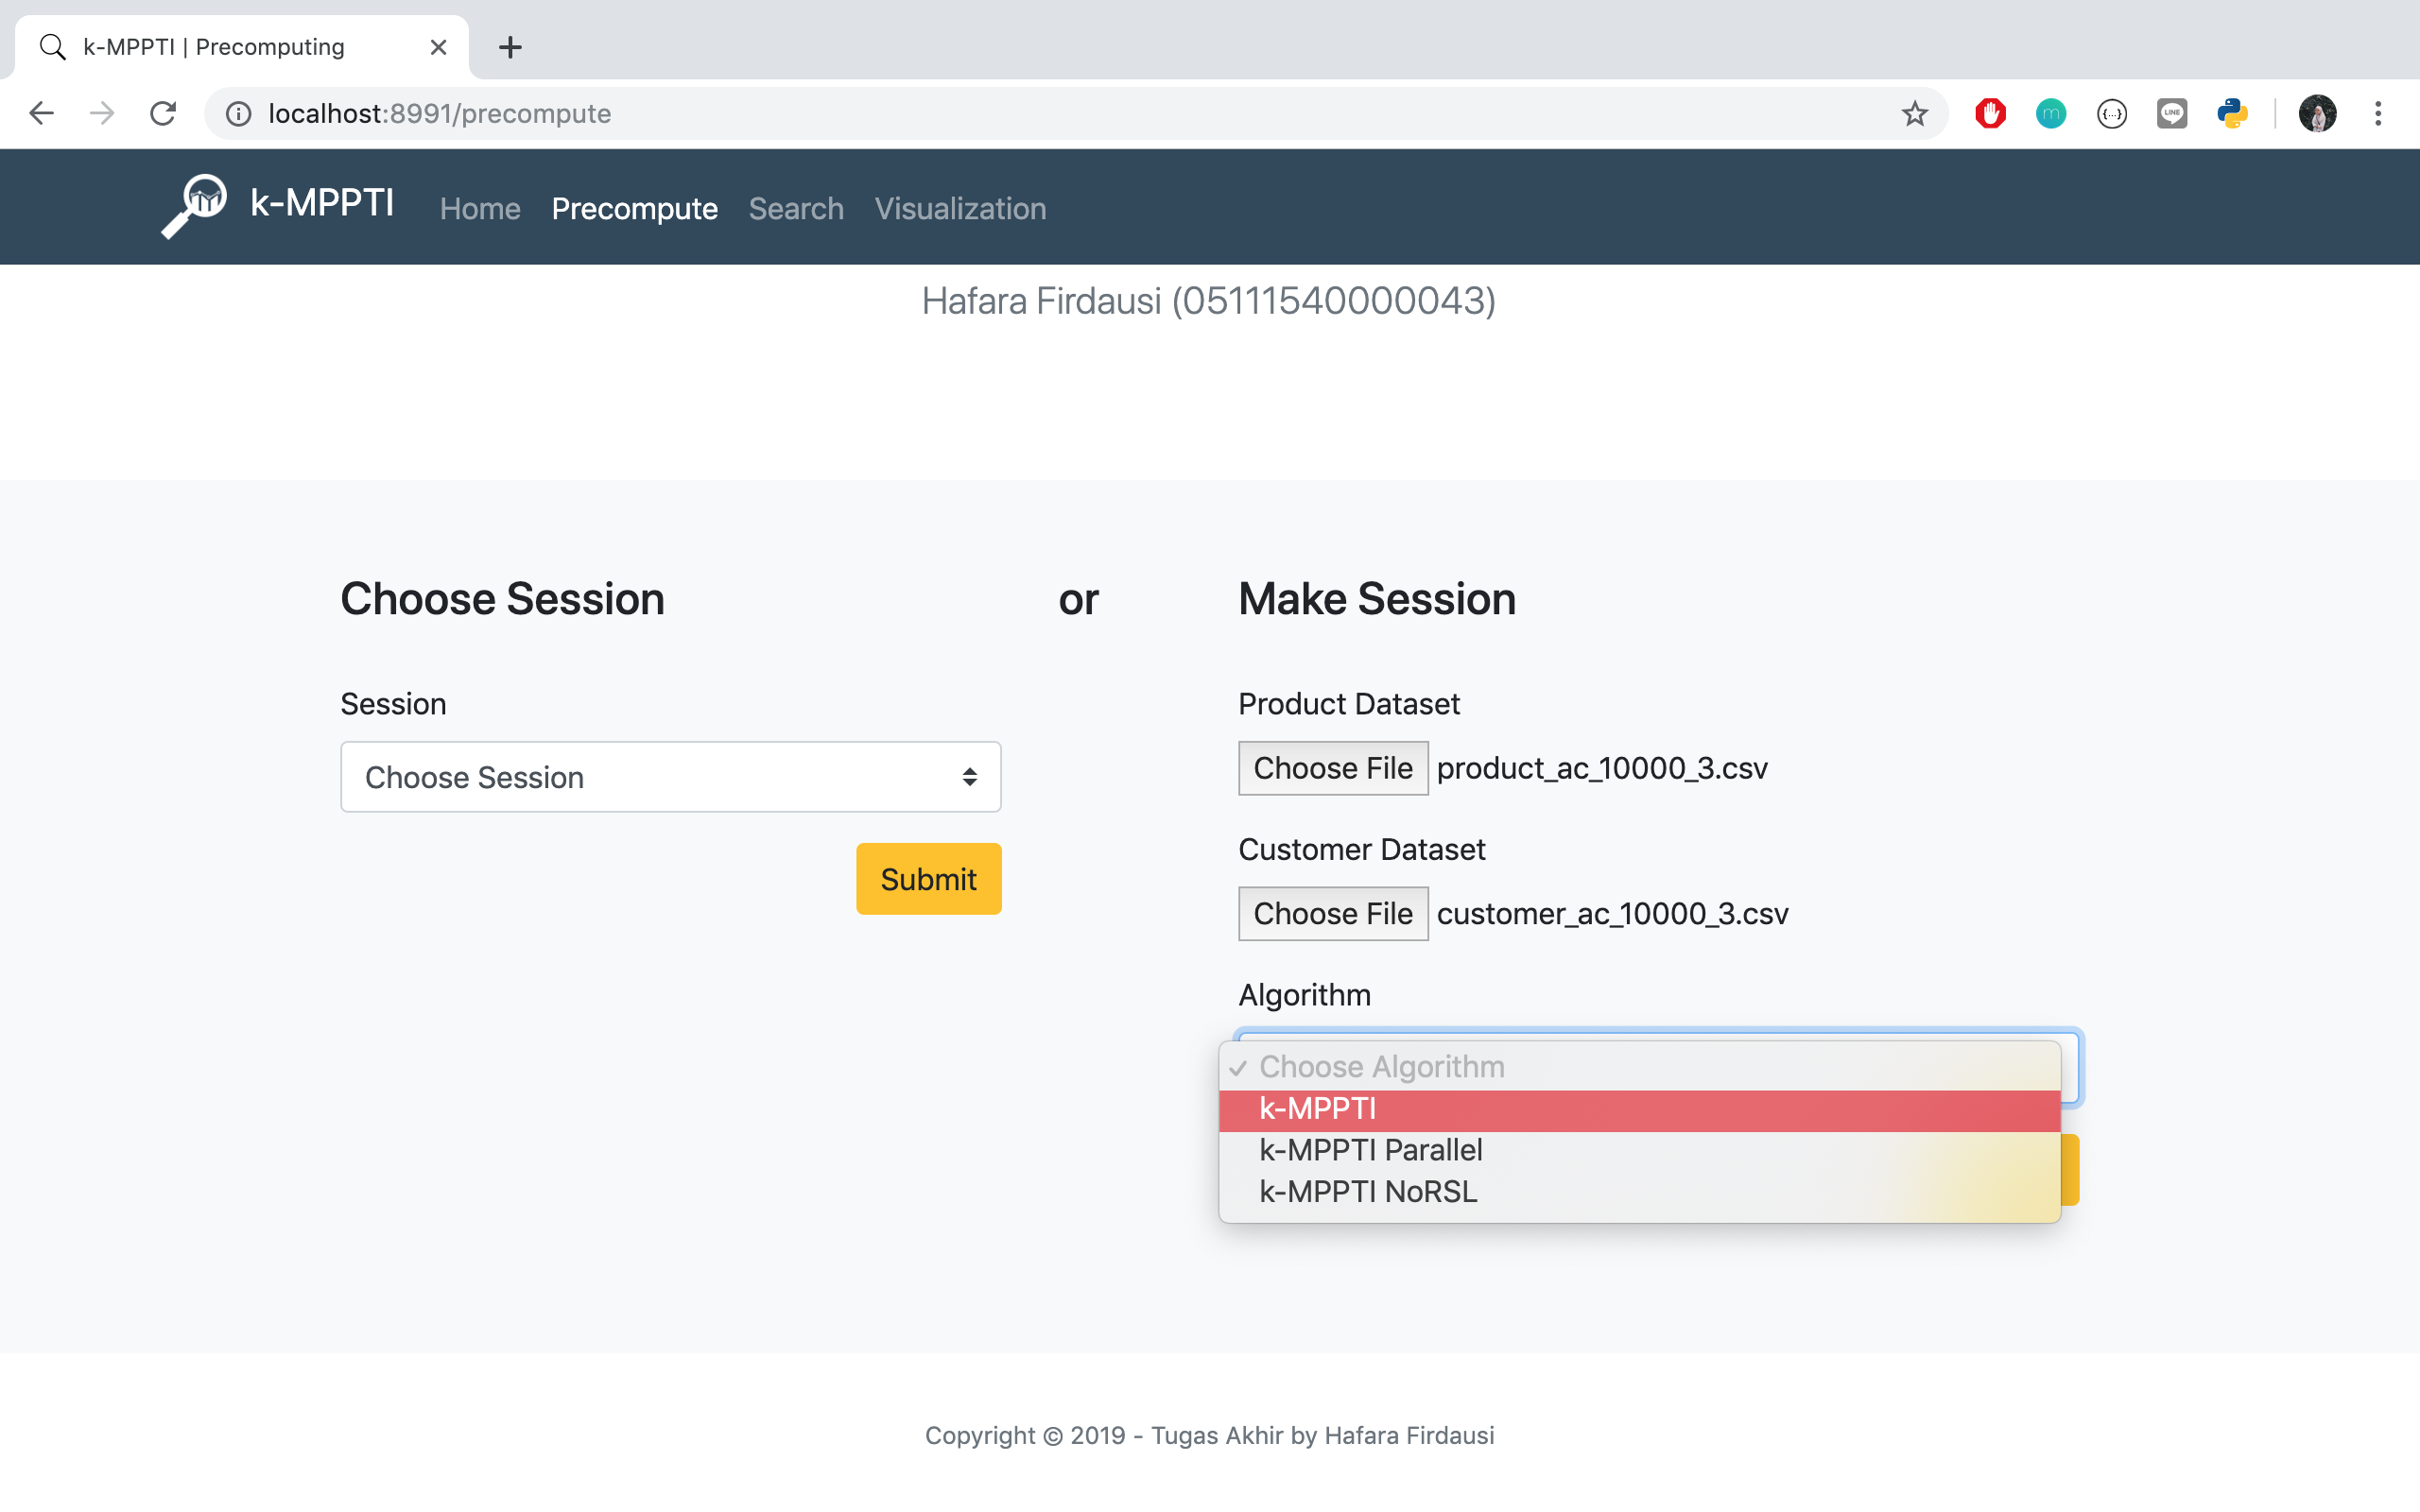
\includegraphics[width=10cm]{assets/img/bab5/hasil2.png}
	\caption{Hasil uji coba: mengunggah data dan memilih algoritme untuk \textit{data precomputing}}
	\label{fig:hasil-performa1}
\end{figure}

\begin{figure}[H]
	\centering
	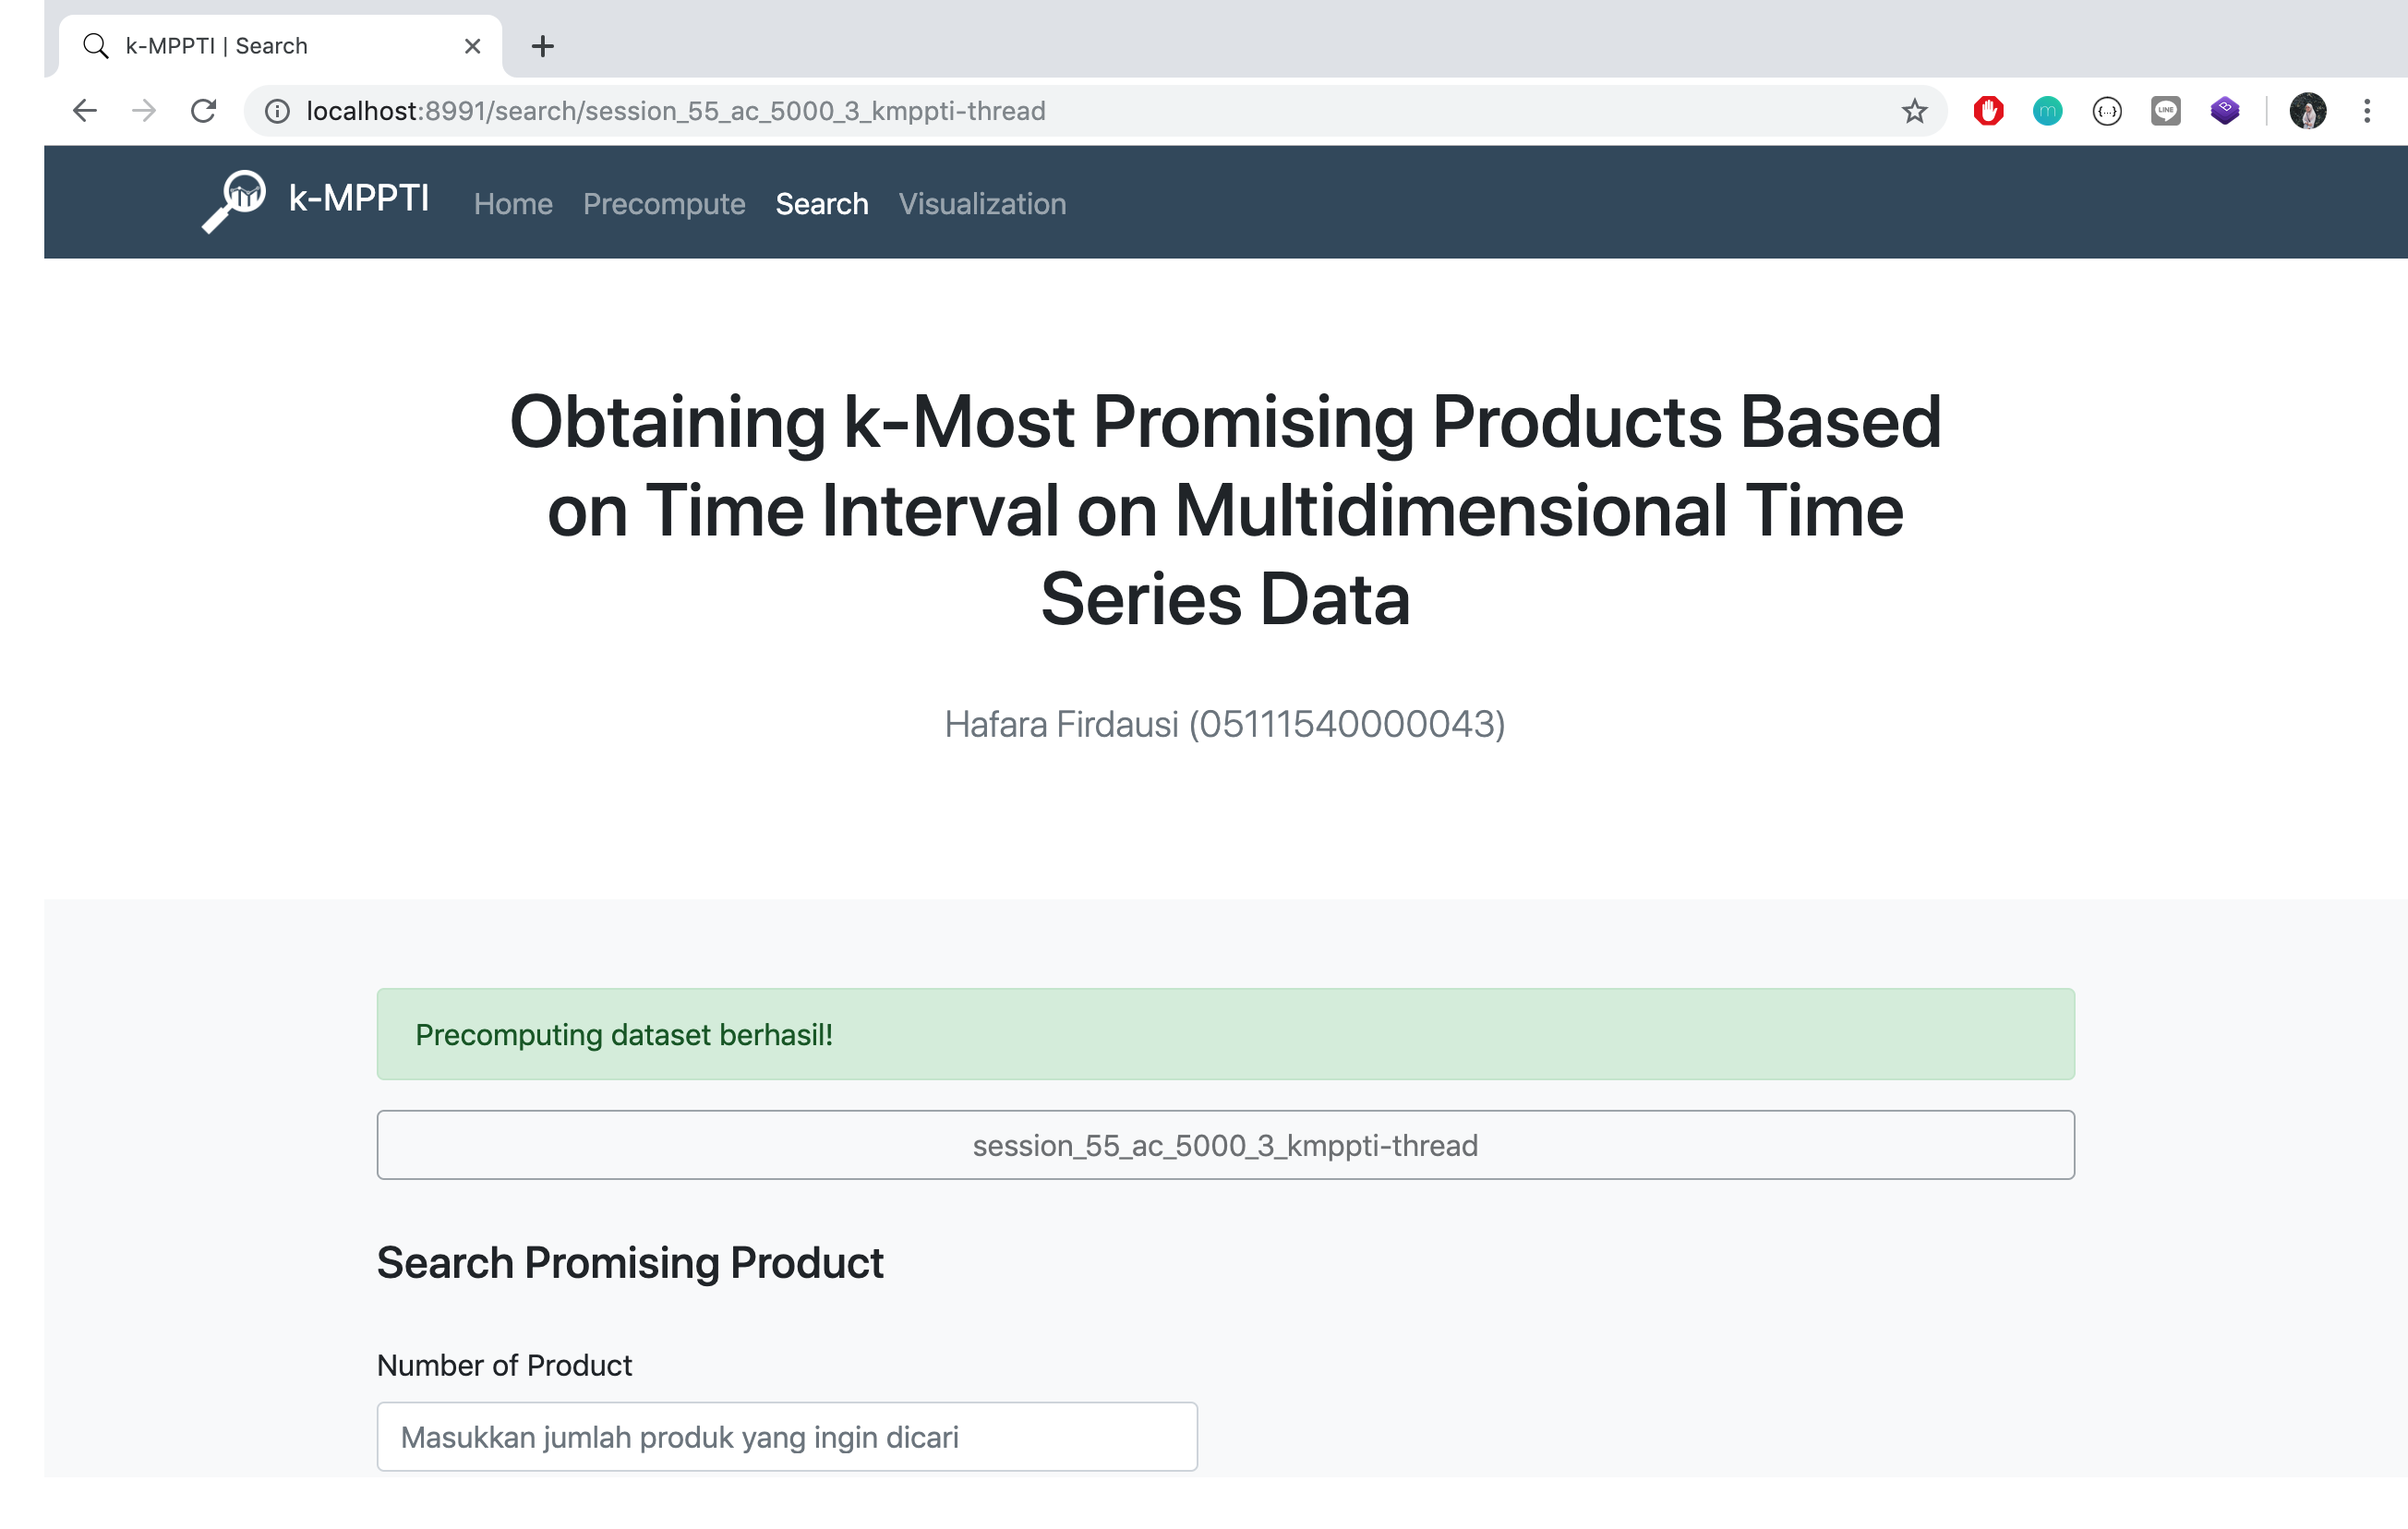
\includegraphics[width=10cm]{assets/img/bab5/hasil1.png}
	\caption{Hasil uji coba: proses \textit{data precomputing} berhasil}
	\label{fig:hasil-performa2}
\end{figure}

\begin{figure}[H]
	\centering
	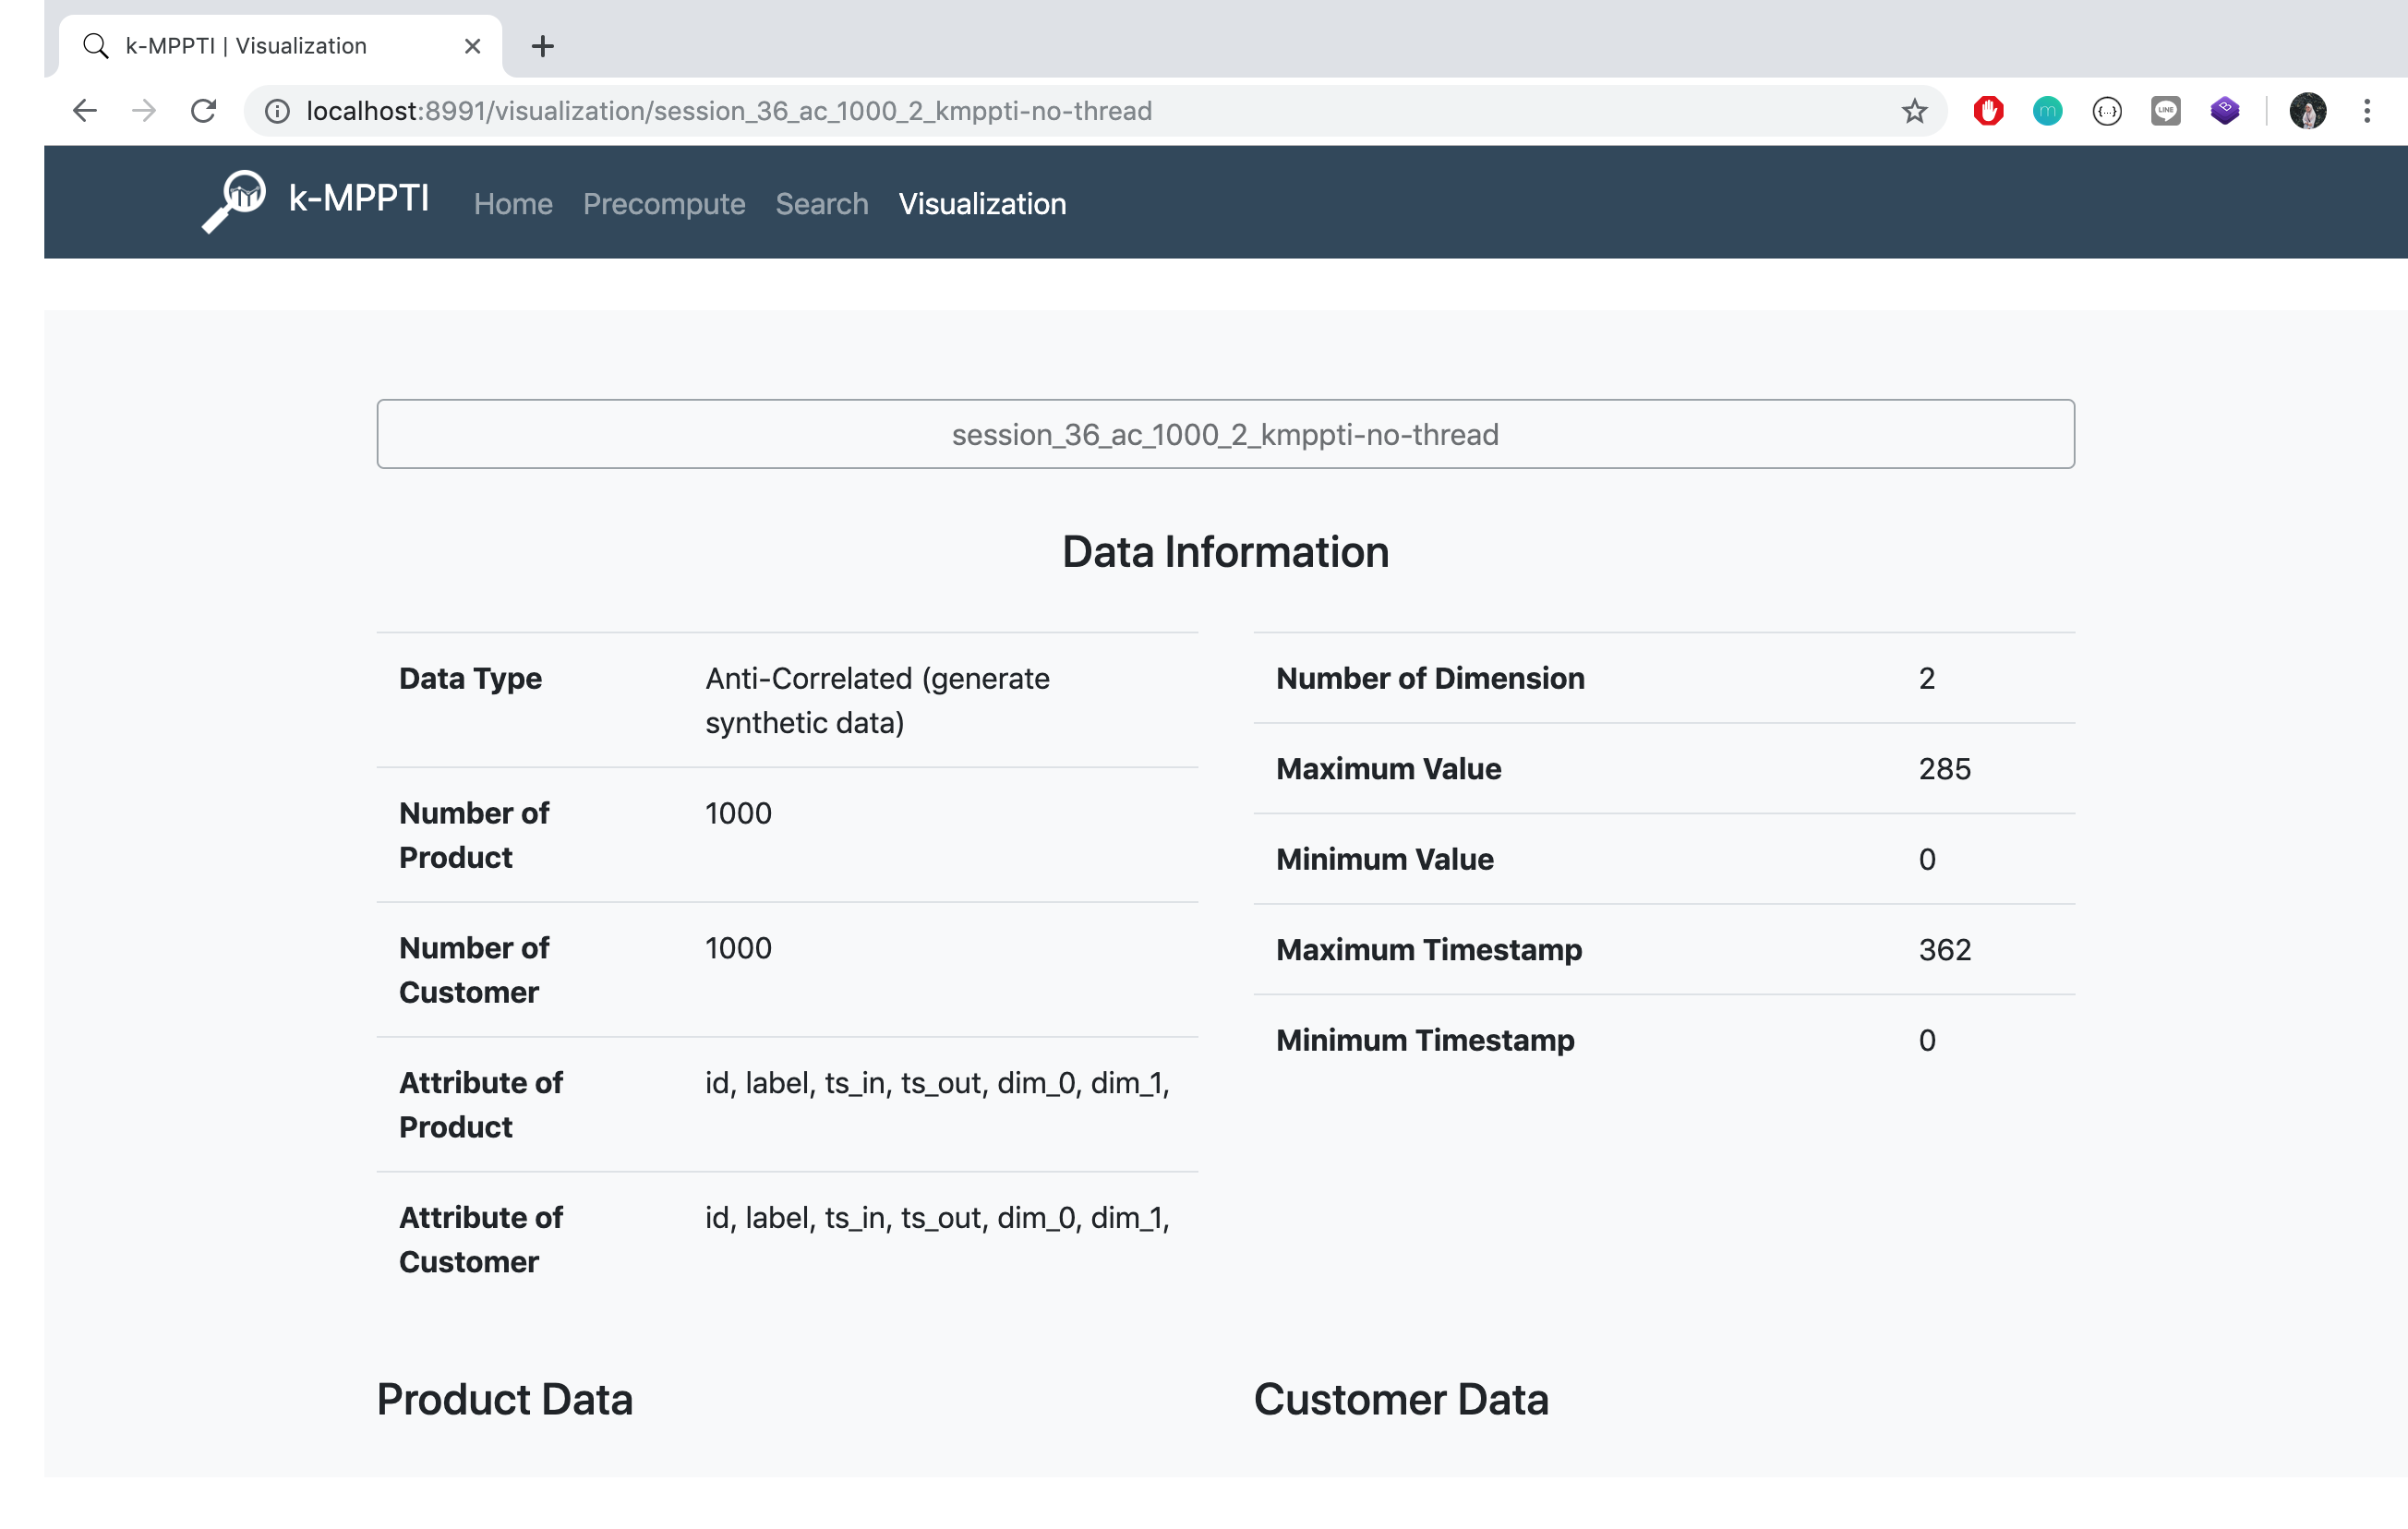
\includegraphics[width=10cm]{assets/img/bab5/hasil3.png}
	\caption{Hasil uji coba: melihat informasi data}
	\label{fig:hasil-performa3}
\end{figure}

\begin{figure}[H]
	\centering
	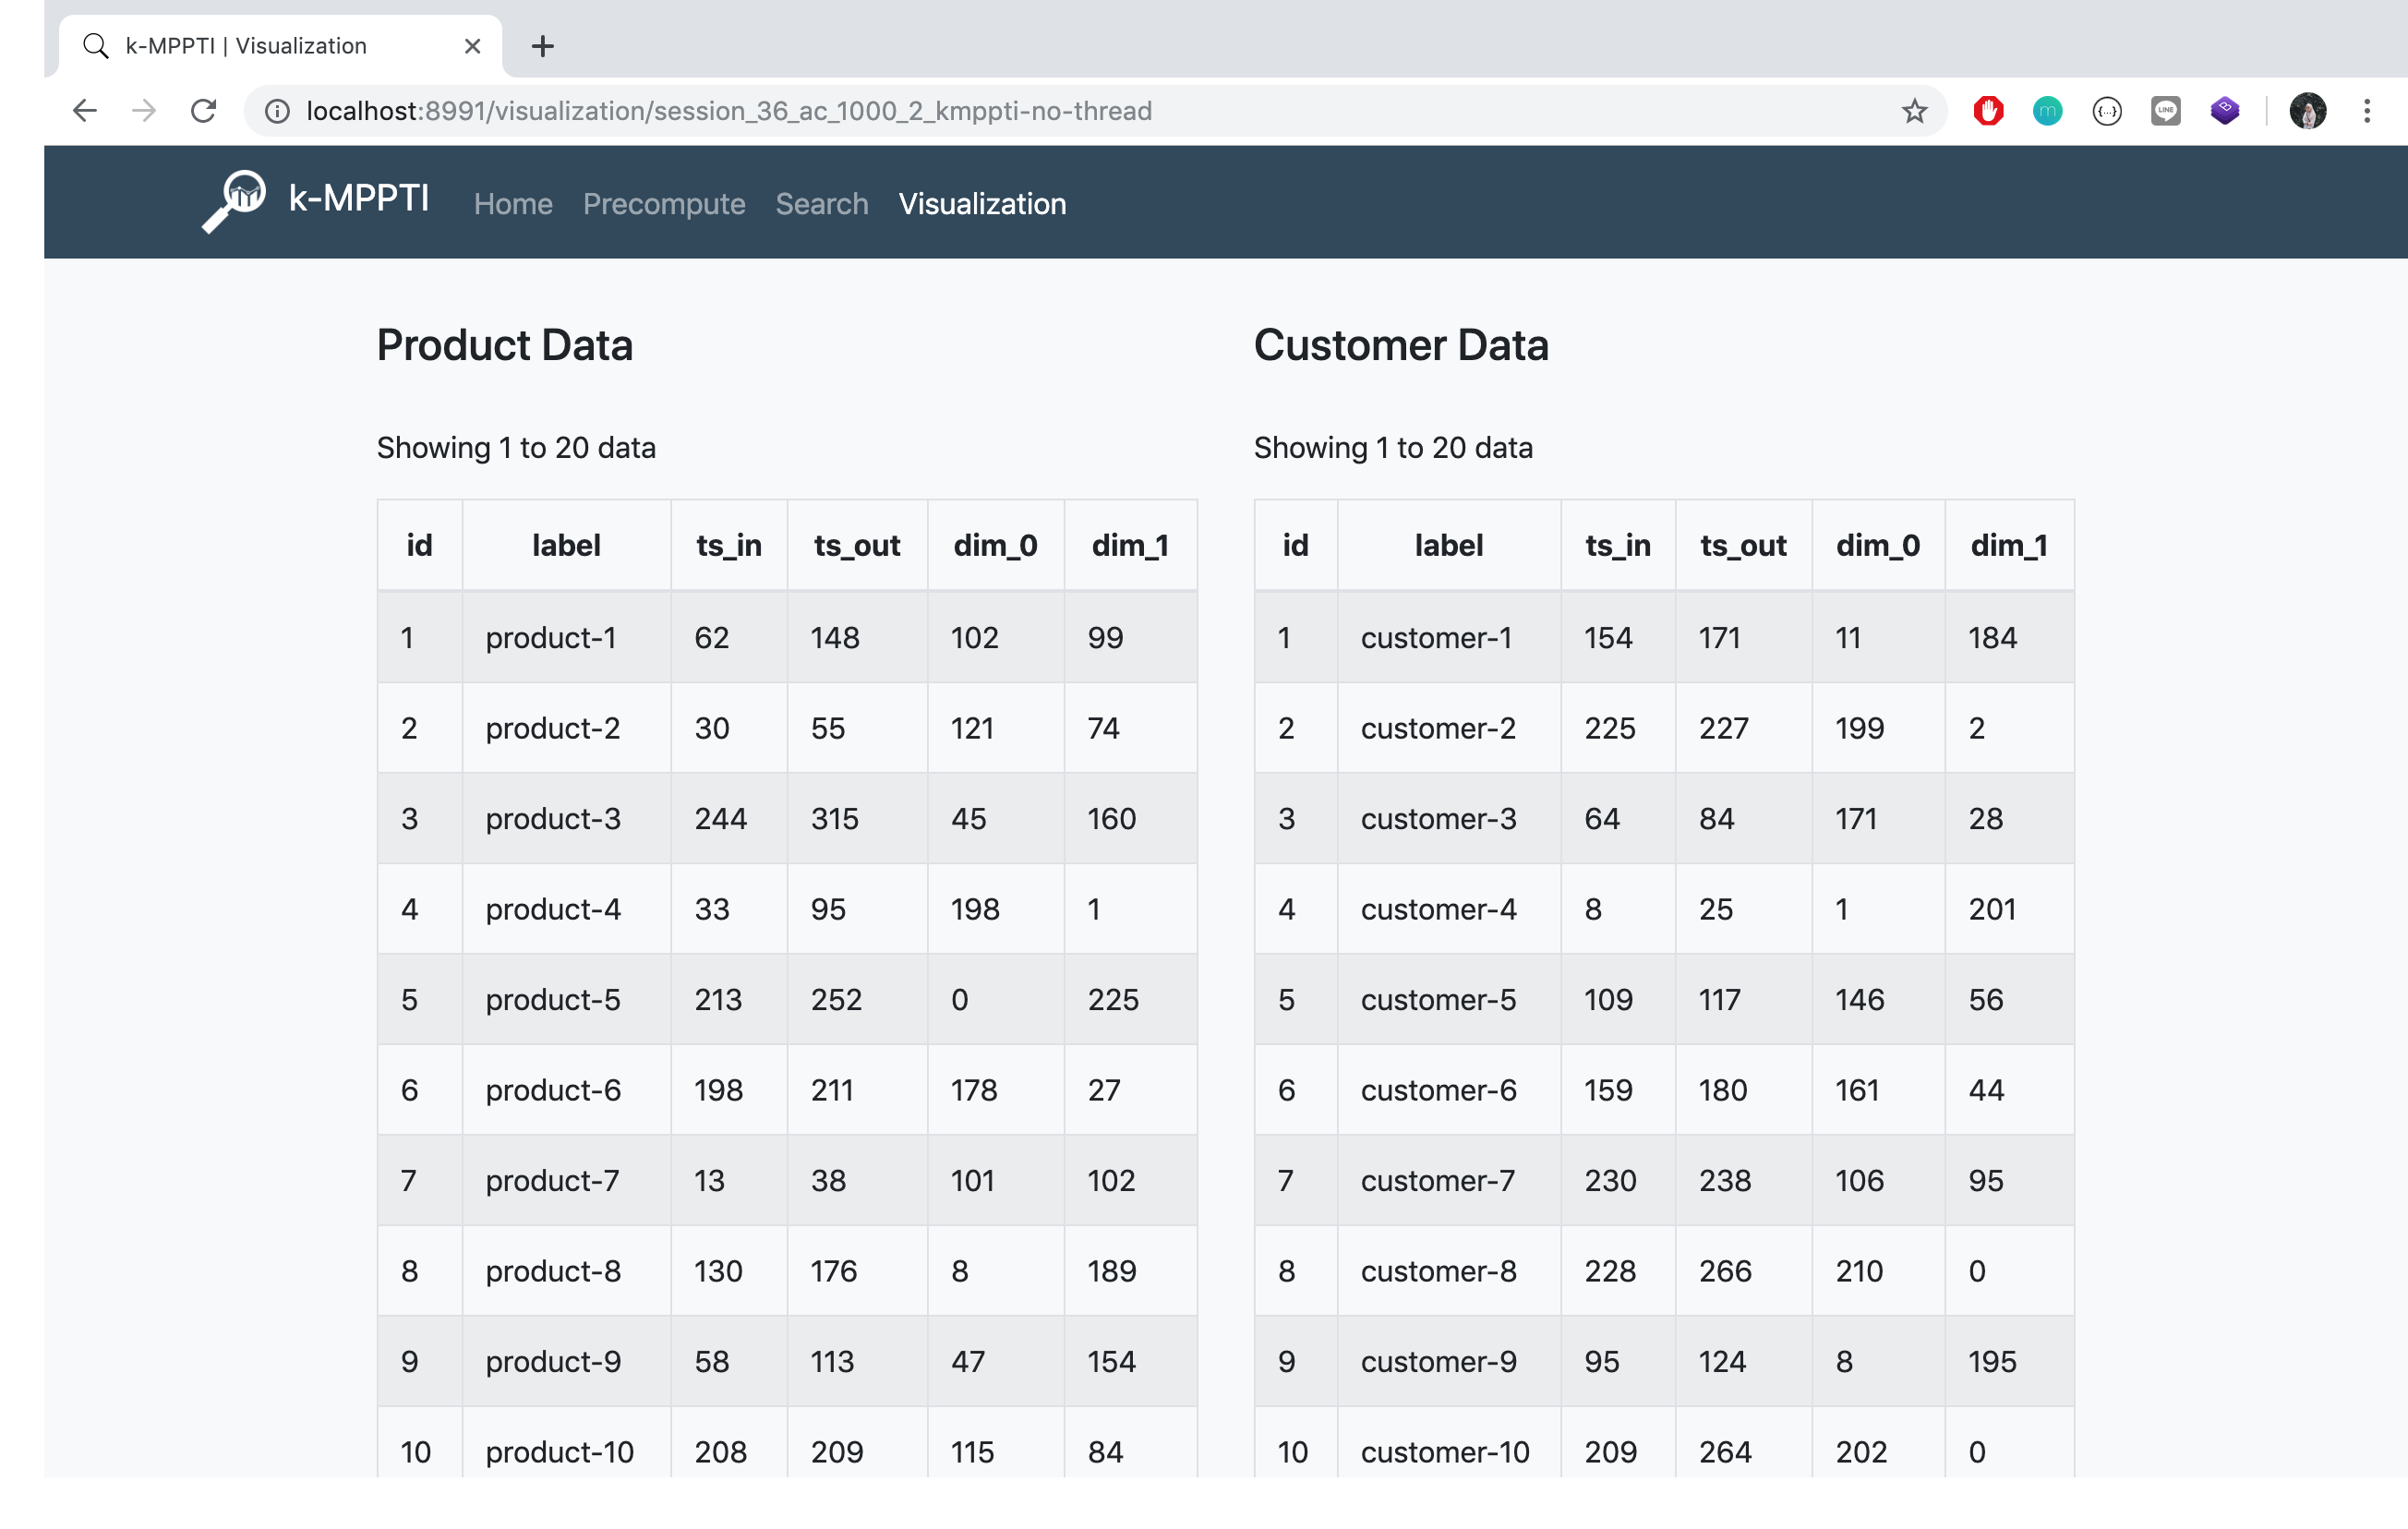
\includegraphics[width=10cm]{assets/img/bab5/hasil4.png}
	\caption{Hasil uji coba: melihat pratinjau data berupa tabel}
	\label{fig:hasil-performa4}
\end{figure}

\begin{figure}[H]
	\centering
	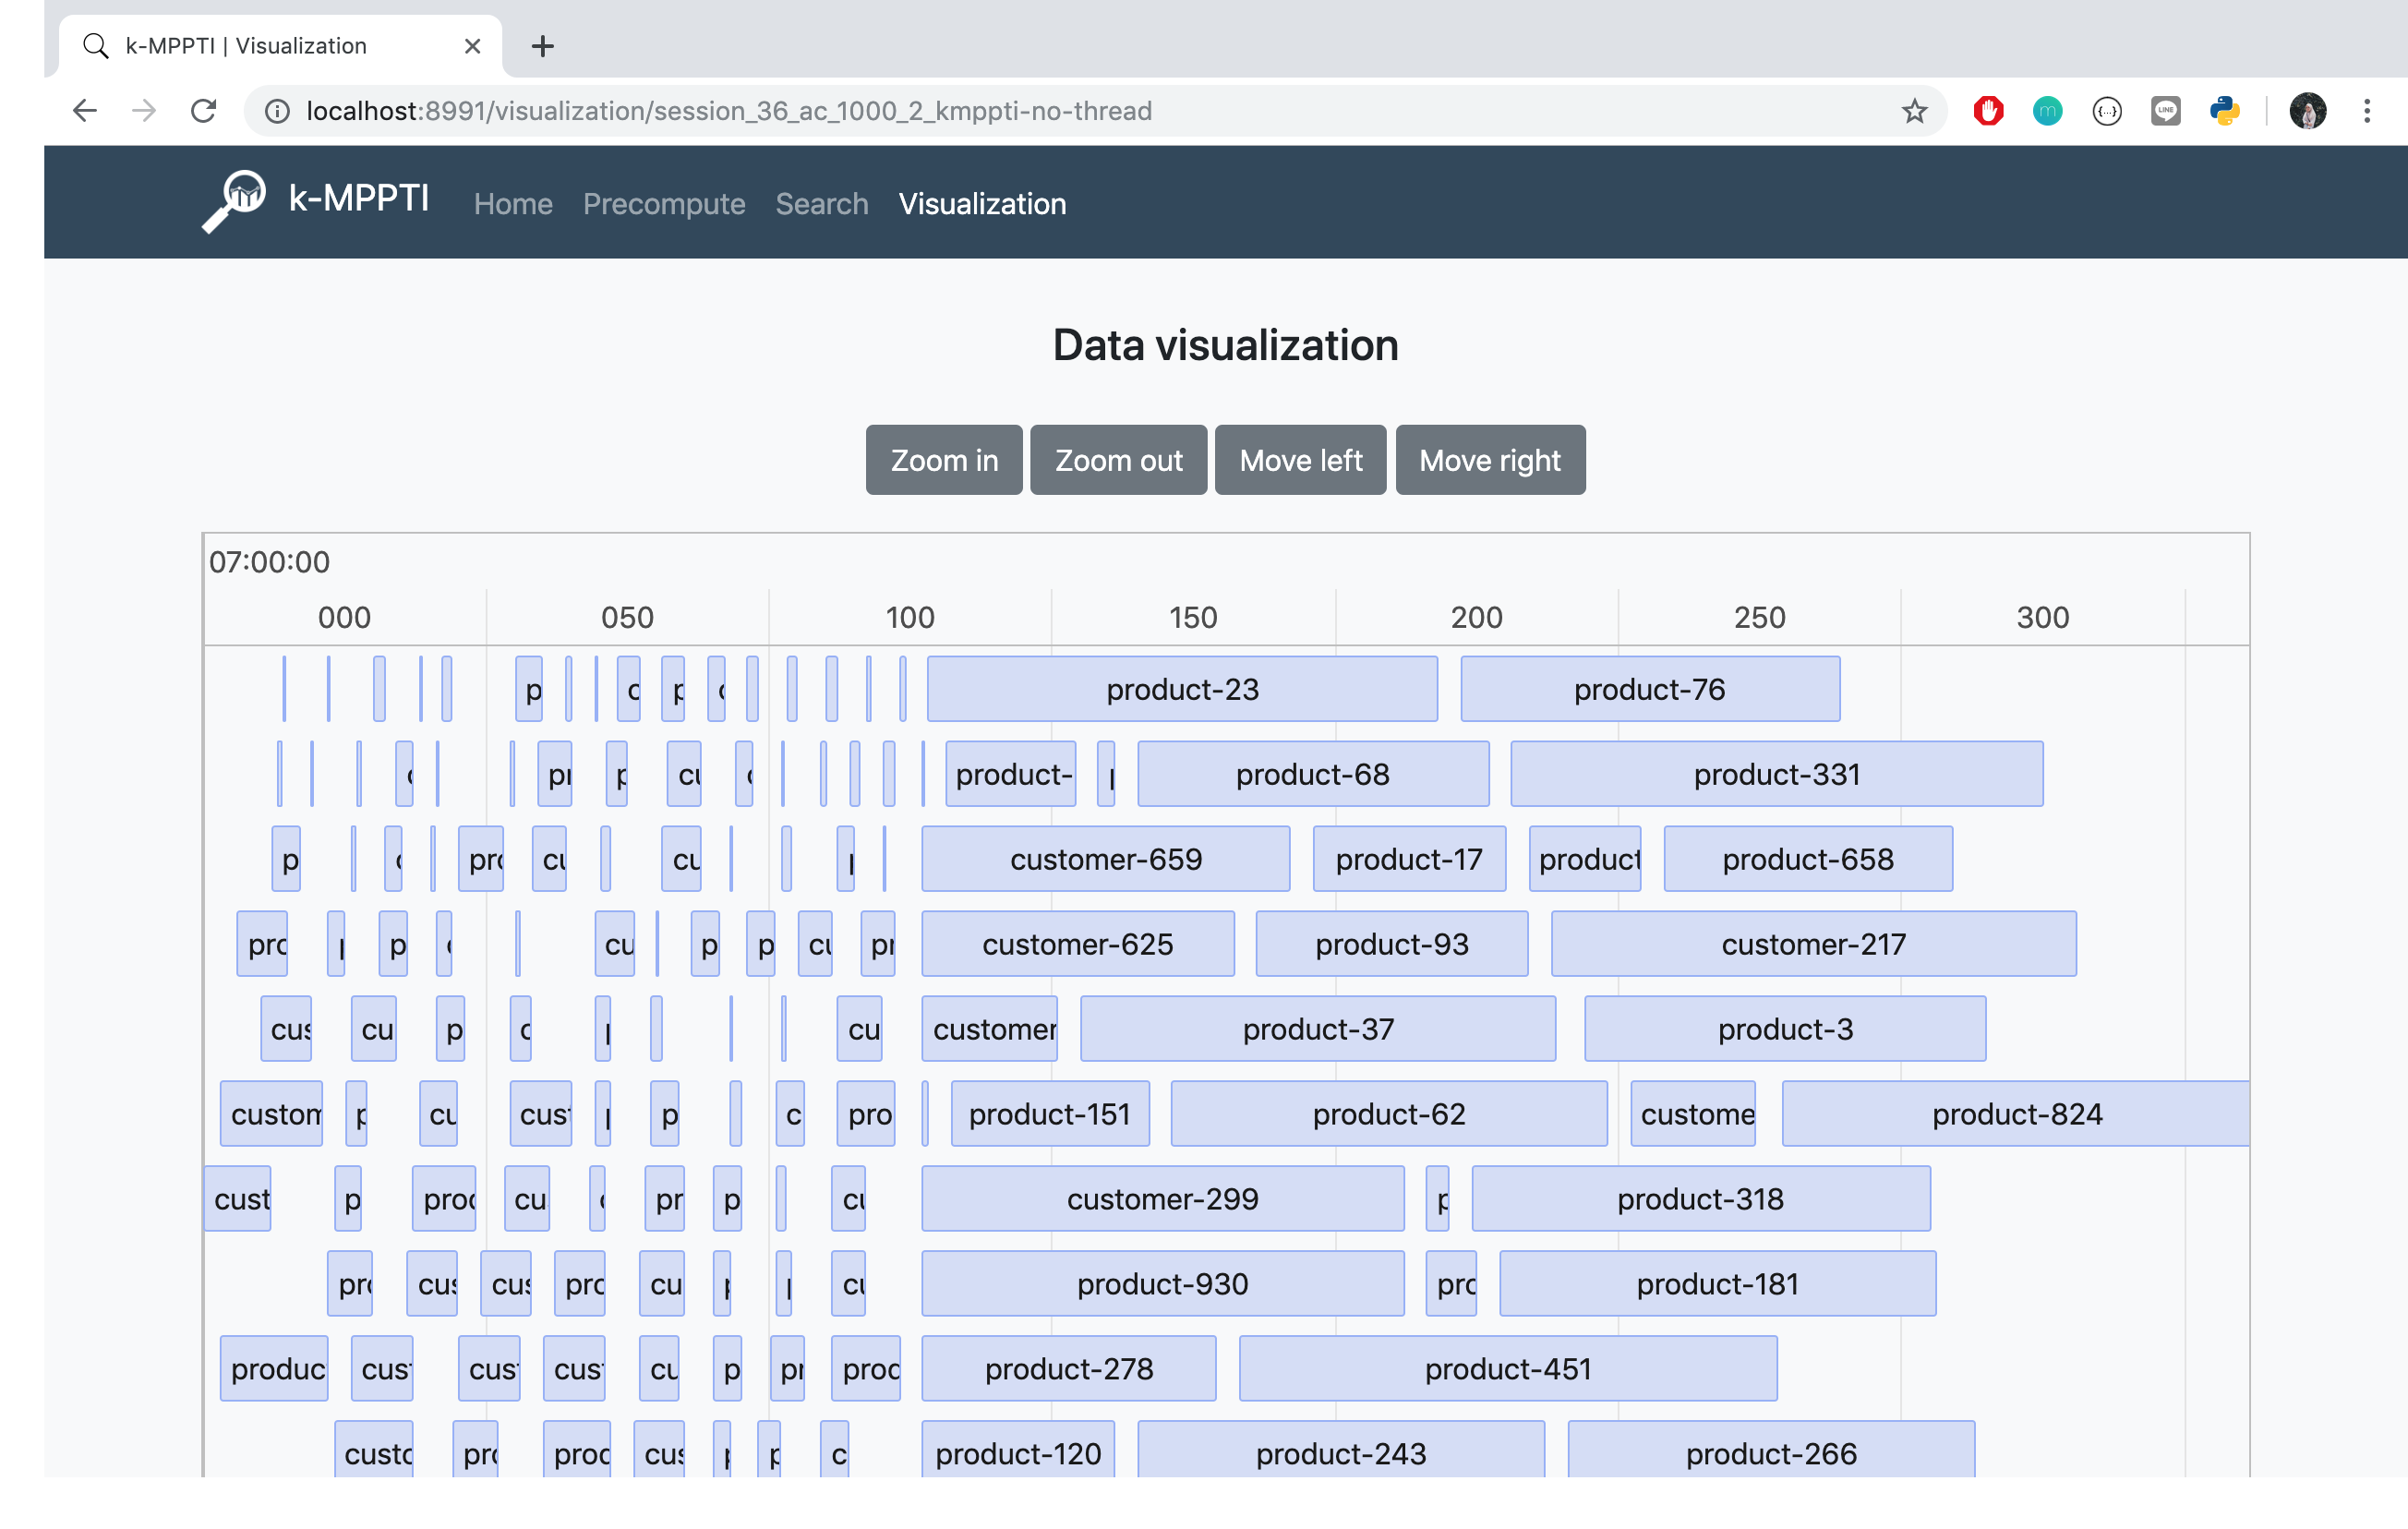
\includegraphics[width=10cm]{assets/img/bab5/hasil5.png}
	\caption{Hasil uji coba: melihat visualisasi data berupa lini masa}
	\label{fig:hasil-performa5}
\end{figure}

\begin{figure}[H]
	\centering
	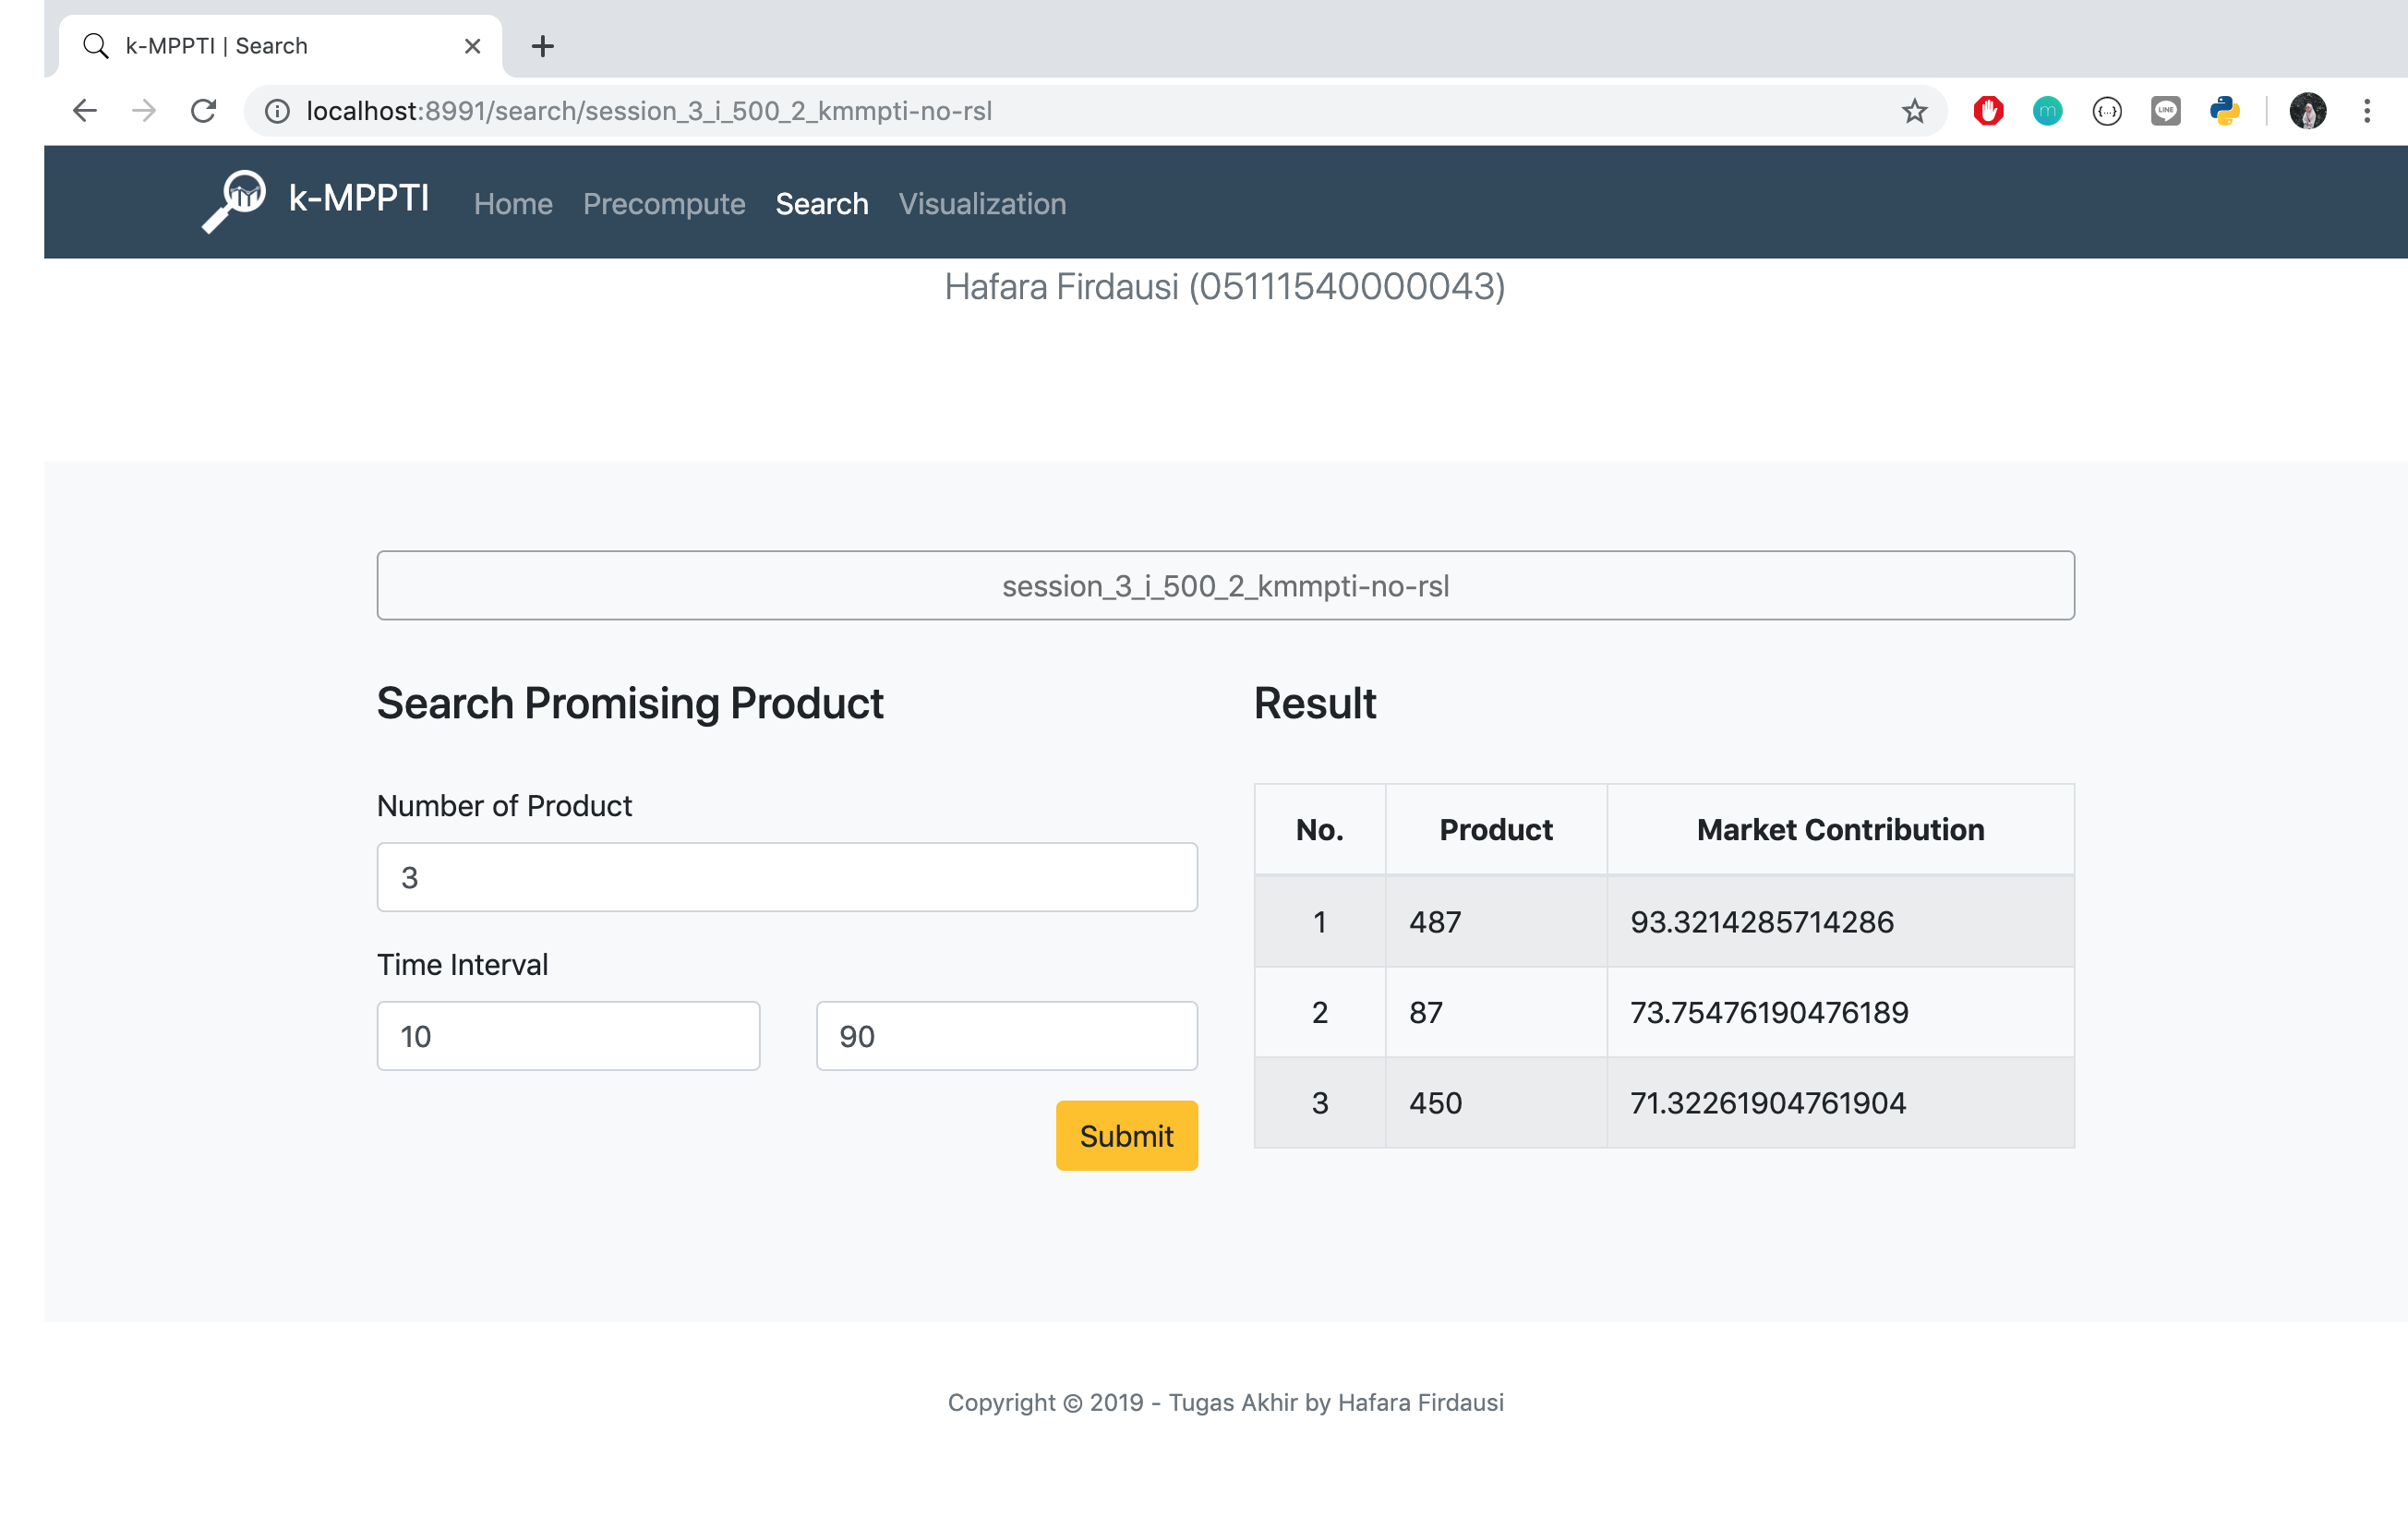
\includegraphics[width=10cm]{assets/img/bab5/hasil6.png}
	\caption{Hasil uji coba: memasukkan kueri pencarian dan melihat hasil kueri}
	\label{fig:hasil-performa6}
\end{figure}

\begin{figure}[H]
	\centering
	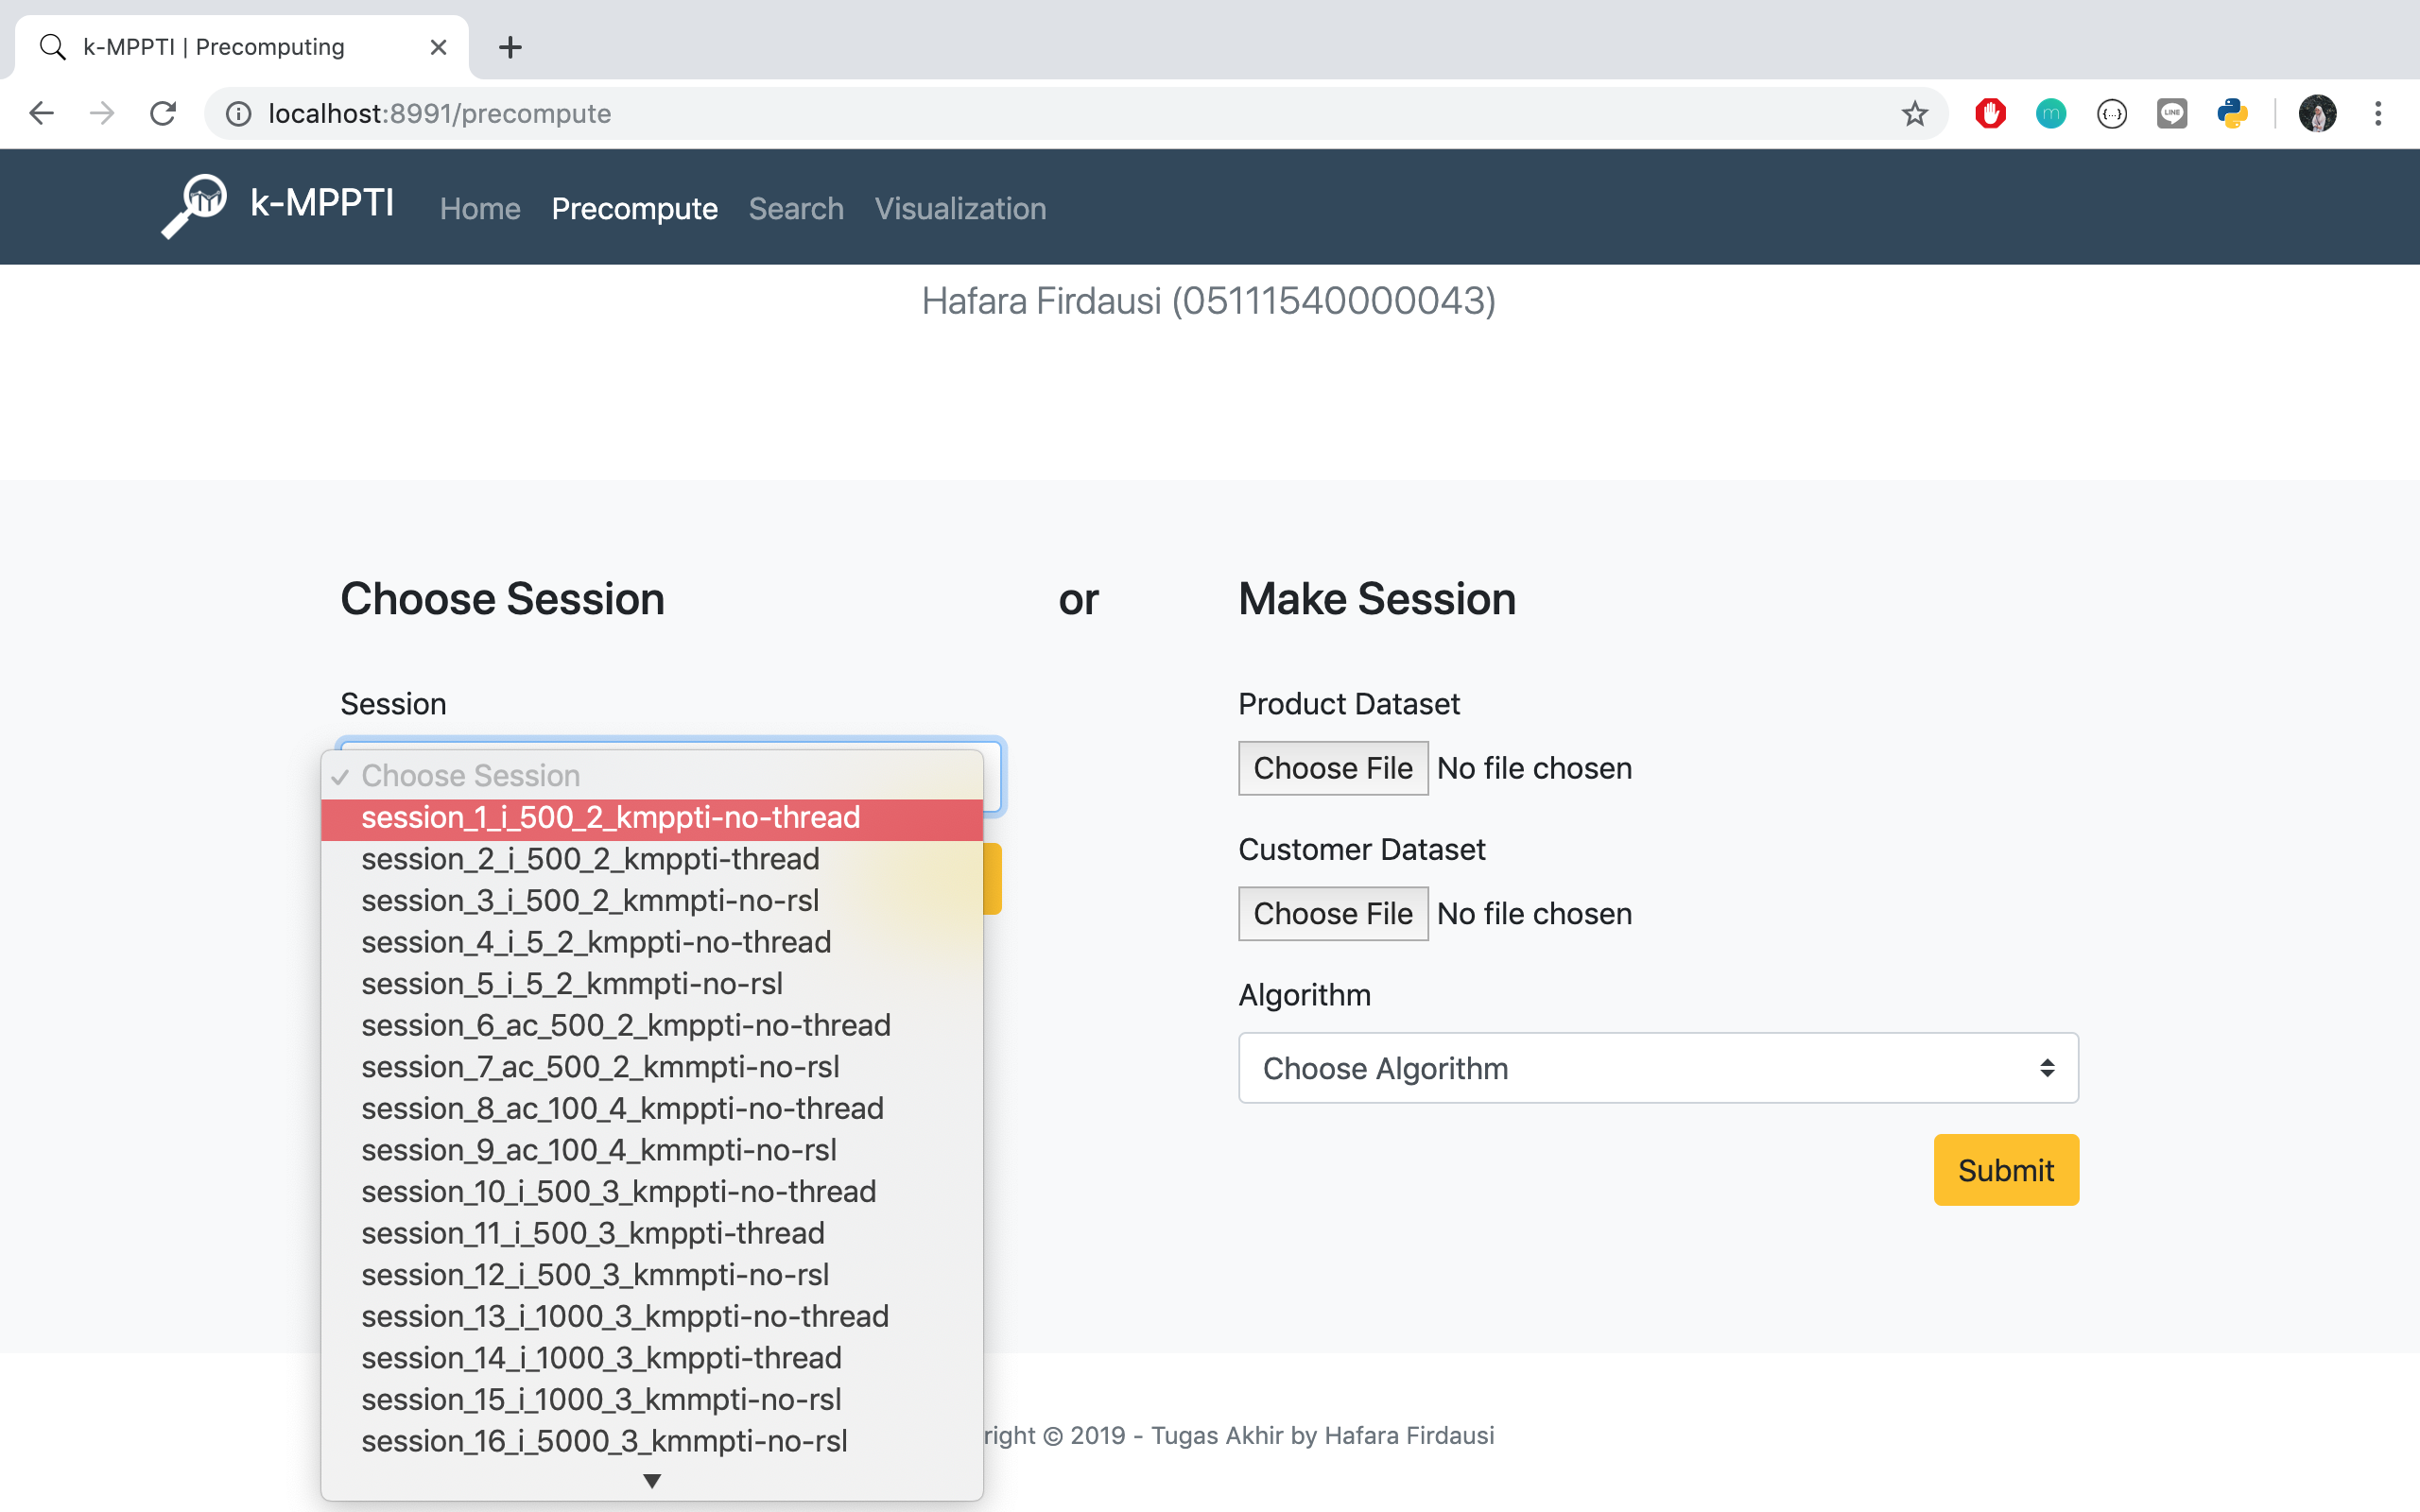
\includegraphics[width=10cm]{assets/img/bab5/hasil7.png}
	\caption{Hasil uji coba: memilih \textit{session}}
	\label{fig:hasil-performa7}
\end{figure}

\subsection{Uji Coba Performa}
\tab Pengujian performa dilakukan sesuai dengan skenario daftar kebutuhan fungsional pada Tabel \ref{tab:uji-coba-performa-precompute} yang hasilnya dianalisis sebagai berikut. 

\subsubsection{Pengaruh Jumlah Data Terhadap Performa Algoritme}

\tab Berdasarkan hasil pengujian menggunakan skenario ke-1, 2, dan 3 pada Tabel \ref{tab:uji-coba-performa-precompute}, dapat diketahui pengaruh perubahan jumlah data terhadap performa masing-masing algoritme. Pengujian ini dilakukan pada ketiga data untuk melihat apakah ada perbedaan yang signifikan antar ketiganya.

Hasil pengujian pada Grafik \ref{fig:grafik-ind-jml-time} dan \ref{fig:grafik-ant-jml-time} menunjukkan bahwa perubahan jumlah data memiliki pengaruh yang sangat signifikan terhadap waktu komputasi. Hal ini terjadi karena semakin banyak data, maka \textit{event} yang harus diproses menjadi empat kali lebih banyak (ada dua data, yakni data produk dan pelanggan). Sebagai contoh, ada 2000 data produk dan pelanggan yang dimasukkan, maka ada 8000 \textit{event} yang harus diproses. Semakin banyak \textit{event} yang diproses, maka semakin lama pula komputasinya.

\begin{figure}[H]
	\centering
	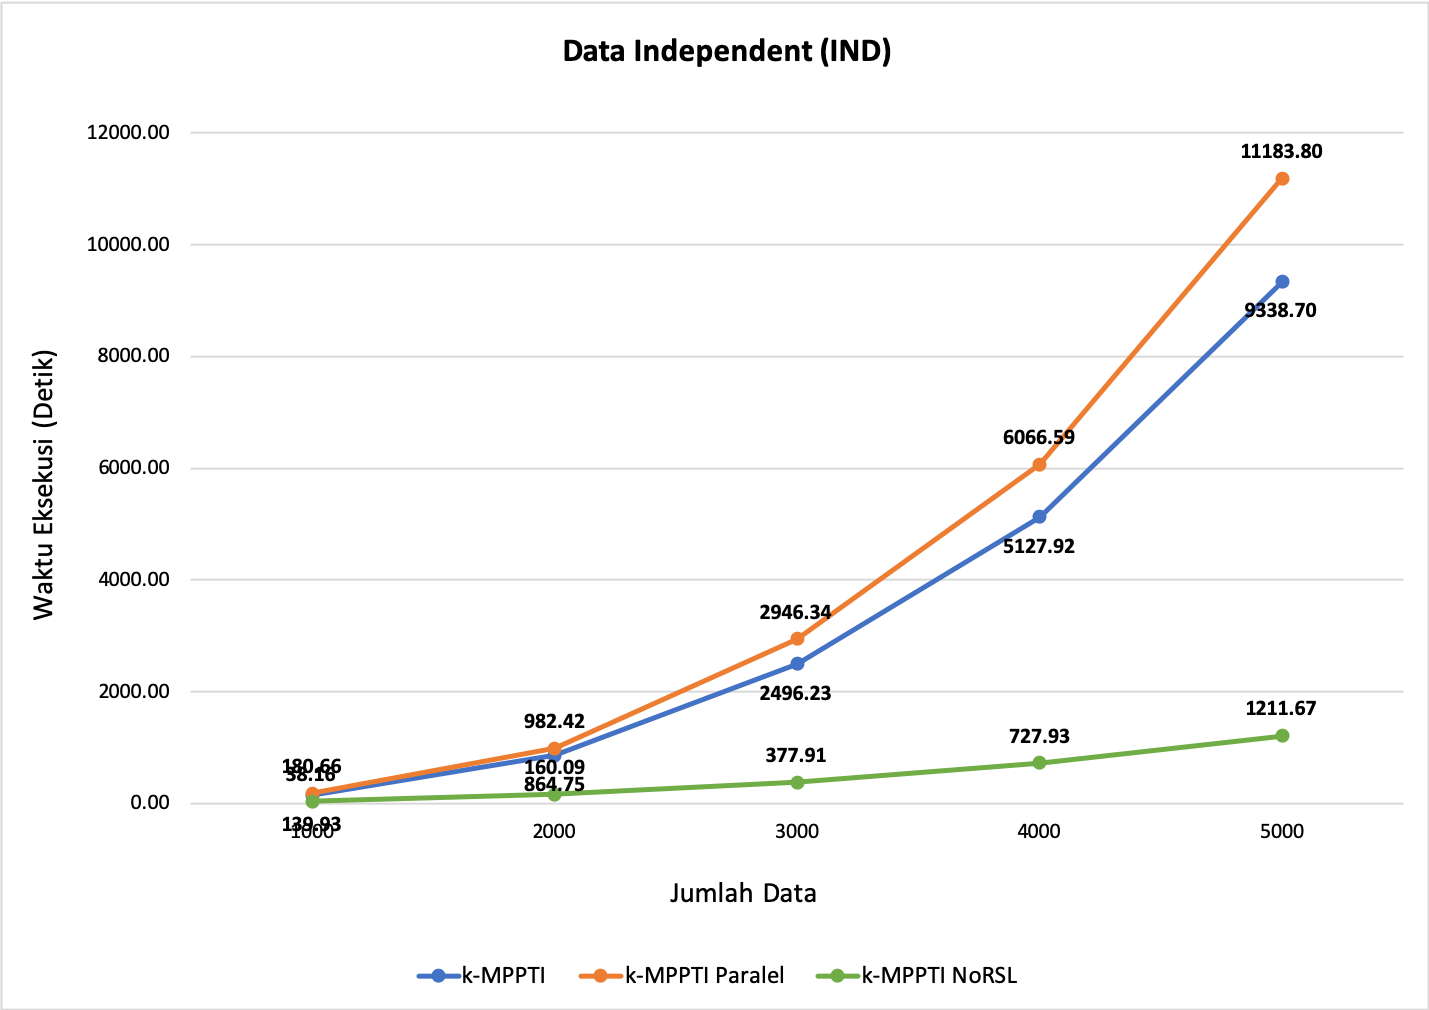
\includegraphics[width=10cm]{assets/img/bab5/grafik-ind-jml-time.png}
	\caption{Grafik pengaruh jumlah data terhadap waktu komputasi algoritme pada data \textit{independent} (IND)}
	\label{fig:grafik-ind-jml-time}
\end{figure}

Jika melihat perbandingan antar data, waktu komputasi pada data \textit{anti-correlated} (ANT) relatif lebih cepat dibandingkan komputasi data \textit{independent} (IND) pada semua algoritme. Namun, data IND memiliki perubahan waktu komputasi yang relatif lebih besar dibandingkan data ANT untuk setiap perubahan jumlah data. Jika diperhatikan lebih dalam lagi, semakin besar jumlah dimensi, maka selisih waktu komputasi antara data IND dan ANT juga semakin besar.

Di sisi lain, jika melihat perbandingan performa algoritme, algoritme k-MPPTI NoRSL memiliki waktu komputasi paling cepat pada semua jenis data dan algoritme k-MPPTI Paralel memiliki waktu komputasi paling lama pada semua jenis data, walaupun tidak terlalu berbeda jauh dengan waktu komputasi k-MPPTI biasa. Padahal hasil kueri ketiganya mirip dan tidak berbeda jauh (dijelaskan pada sub bagian \ref{hasil-kueri}).

\begin{figure}[H]
	\centering
	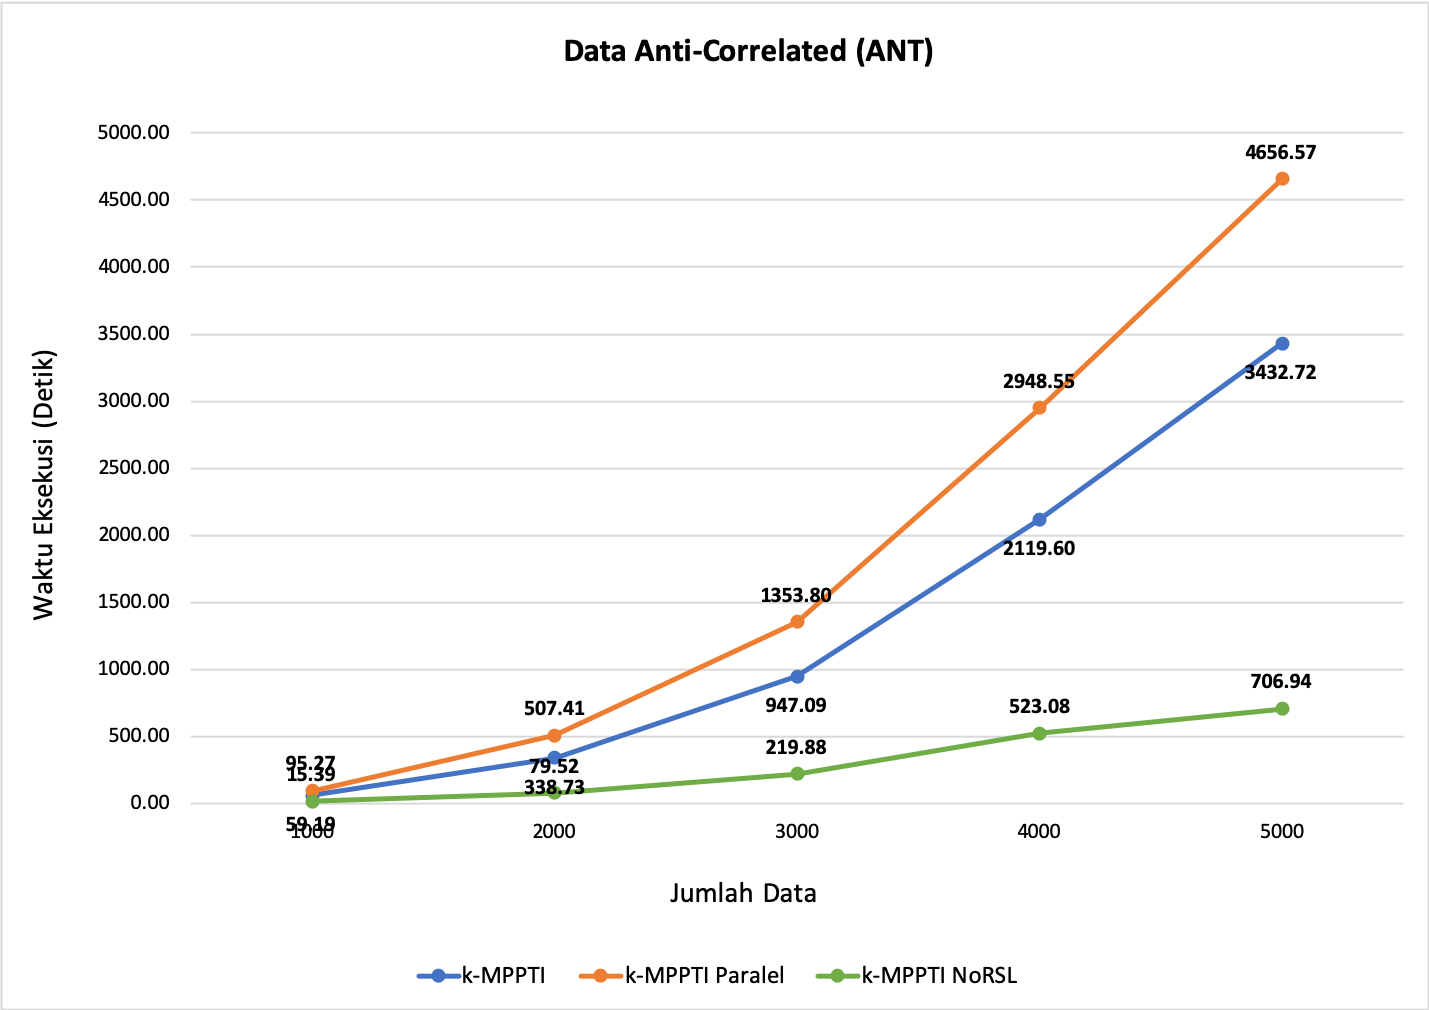
\includegraphics[width=10cm]{assets/img/bab5/grafik-ant-jml-time.png}
	\caption{Grafik pengaruh jumlah data terhadap waktu komputasi algoritme pada data \textit{anti-correlated} (ANT)}
	\label{fig:grafik-ant-jml-time}
\end{figure}

Algoritme k-MPPTI paralel memiliki waktu komputasi paling lama dibandingkan kedua algoritme yang lain karena teknik komputasi paralel diimplementasikan hanya menggunakan satu \textit{resource} menggunakan \textit{thread}, sehingga lebih memberatkan CPU karena harus membagi \textit{resource}-nya. Lambatnya waktu eksekusi berbanding lurus dengan jumlah data karena \textit{thread} dibentuk sejumlah data pelanggan, sehingga semakin banyak data, maka semakin banyak pula \textit{thread} yang terbentuk.

\begin{figure}[H]
	\centering
	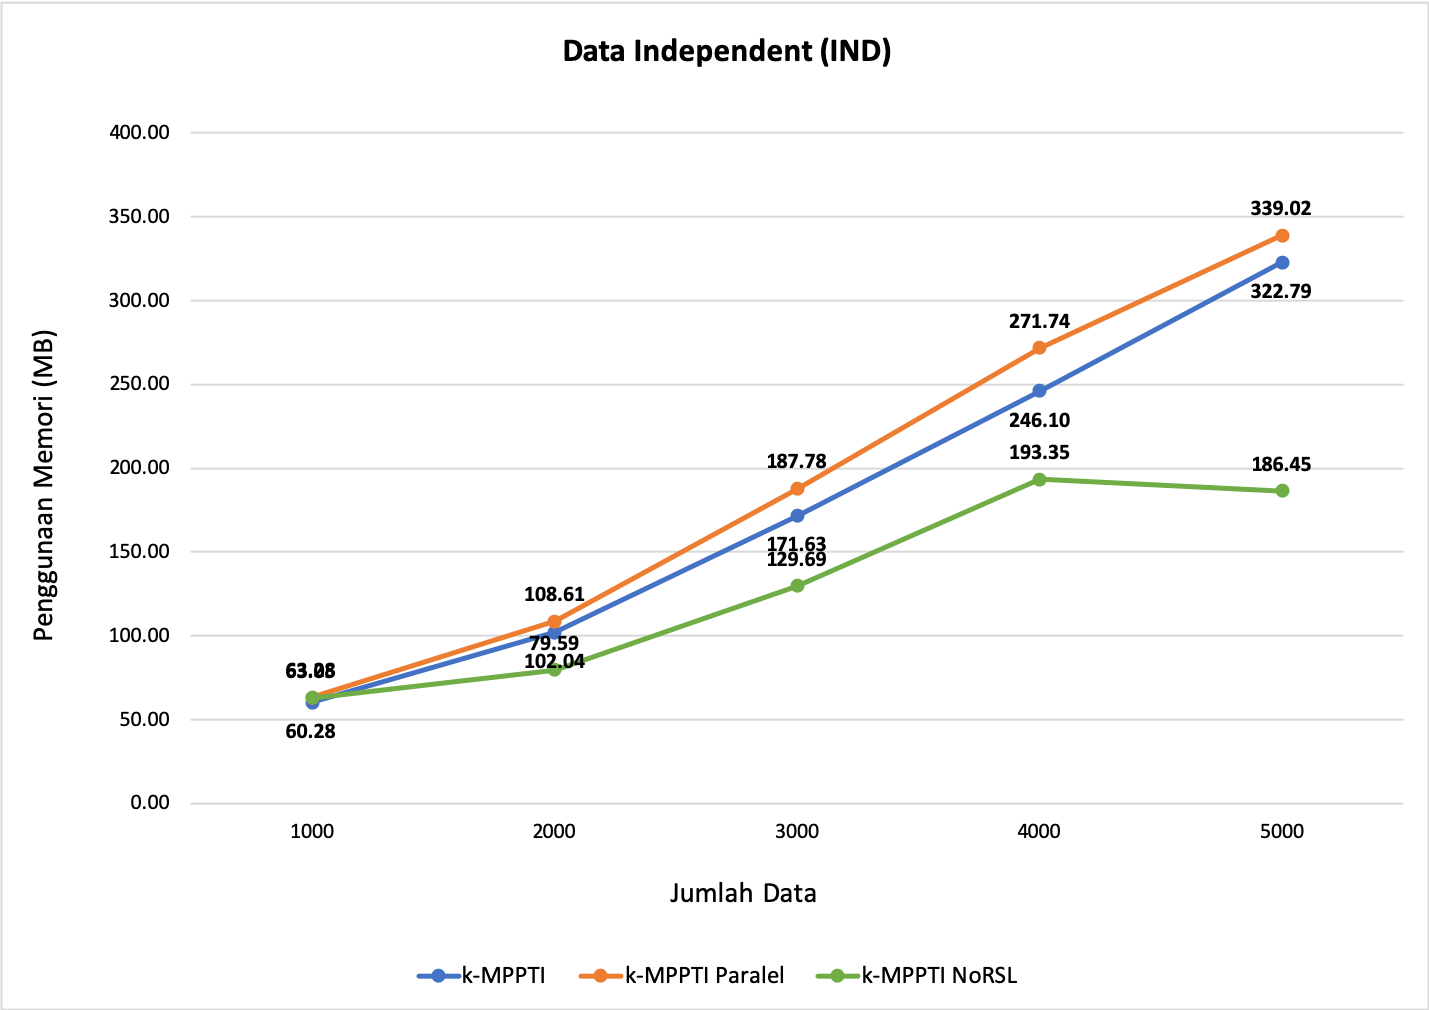
\includegraphics[width=10cm]{assets/img/bab5/grafik-ind-jml-mem.png}
	\caption{Grafik pengaruh jumlah data terhadap penggunaan memori algoritme pada data \textit{independent} (IND)}
	\label{fig:grafik-ind-jml-mem}
\end{figure}

\begin{figure}[H]
	\centering
	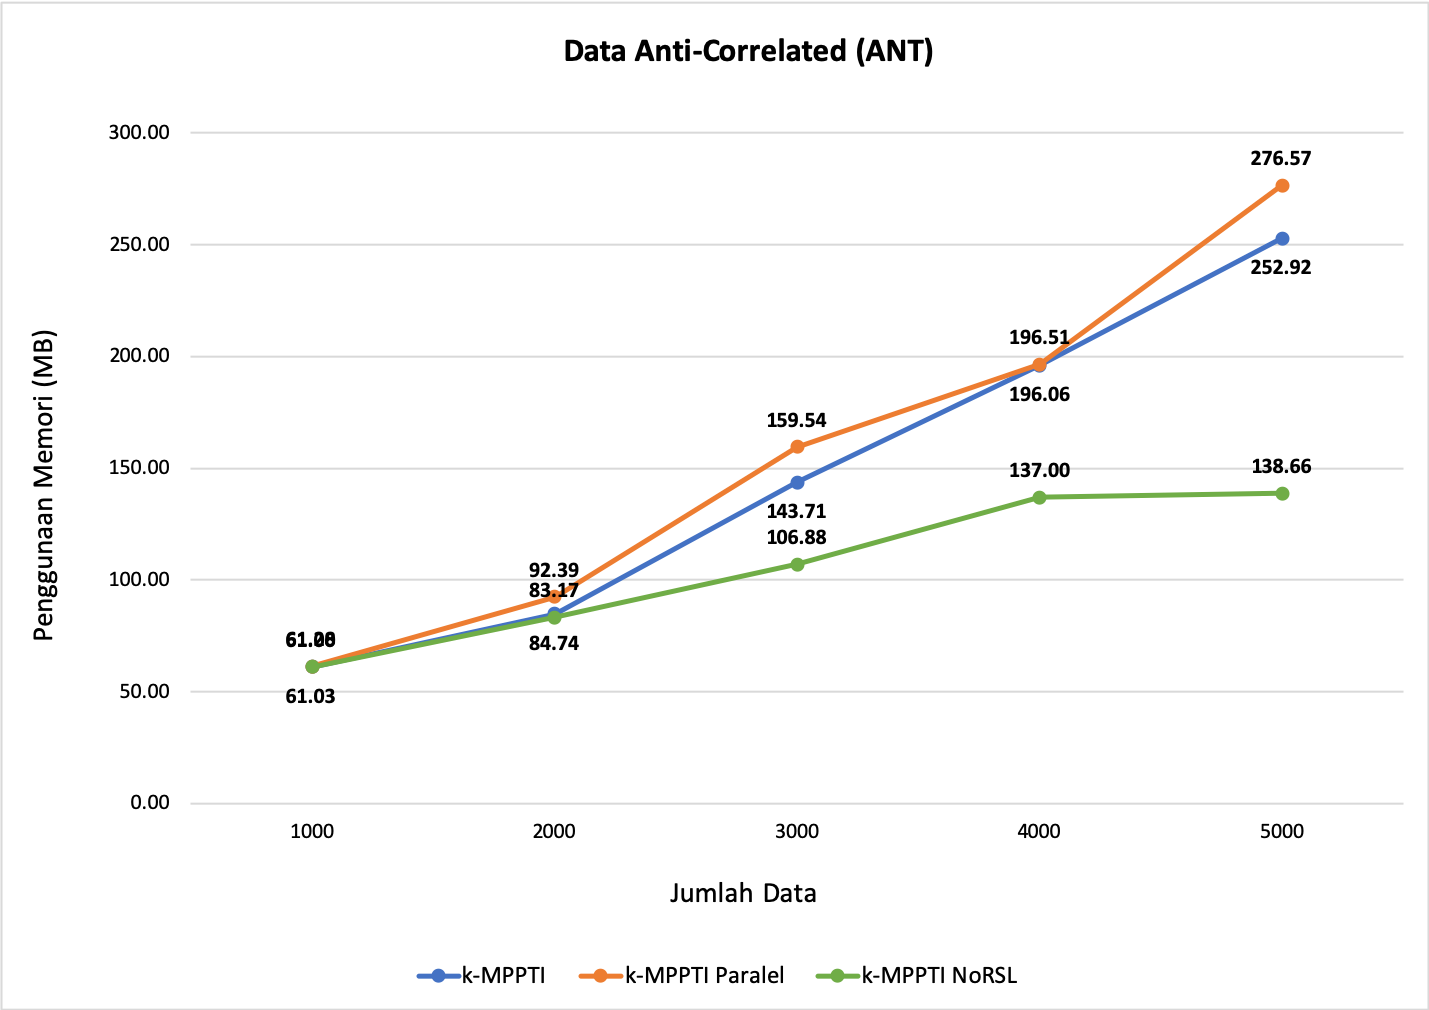
\includegraphics[width=10cm]{assets/img/bab5/grafik-ant-jml-mem.png}
	\caption{Grafik pengaruh jumlah data terhadap penggunaan memori algoritme pada data \textit{anti-correlated} (ANT)}
	\label{fig:grafik-ant-jml-mem}
\end{figure}

Hasil uji coba pengaruh perubahan jumlah data terhadap penggunaan memori algoritme ditunjukkan oleh Grafik \ref{fig:grafik-ind-jml-mem} dan \ref{fig:grafik-ant-jml-mem}. Dalam grafik tersebut, perubahan memori terjadi secara signifikan pada kedua data IND dan ANT. Perubahan memori cenderung berbanding lurus dengan perubahan jumlah data, namun menunjukkan ketidakstabilan pada kedua data.
Sama seperti sebelumnya, penggunaan memori pada data IND cenderung lebih banyak dibandingkan data ANT.

\subsubsection{Pengaruh Jumlah Dimensi Data Terhadap Performa Algoritme}

\tab Berdasarkan hasil pengujian menggunakan skenario ke-4, 5, dan 6 pada Tabel \ref{tab:uji-coba-performa-precompute}, dapat diketahui pengaruh perubahan jumlah dimensi data terhadap performa masing-masing algoritme. Pengujian ini dilakukan pada ketiga data untuk melihat apakah ada perbedaan yang signifikan antar ketiganya. 

Hasil pengujian pada Grafik \ref{fig:grafik-ind-dim-time} dan \ref{fig:grafik-ant-dim-time} menunjukkan bahwa perubahan jumlah dimensi data memiliki pengaruh yang sangat signifikan terhadap waktu komputasi. Hal ini dikarenakan jumlah dimensi sangat berpengaruh terhadap penentuan dominansi antar data, sehingga nilai setiap dimensi harus dibandingkan satu per-satu. Selain itu, iterasi setiap dimensi dilakukan dua kali. Pertama untuk menghitung selisih (selanjutnya disimpan dalam struktur data supaya dapat digunakan kembali tanpa komputasi ulang). Kedua untuk mengecek dominansi antar produk.

\begin{figure}[H]
	\centering
	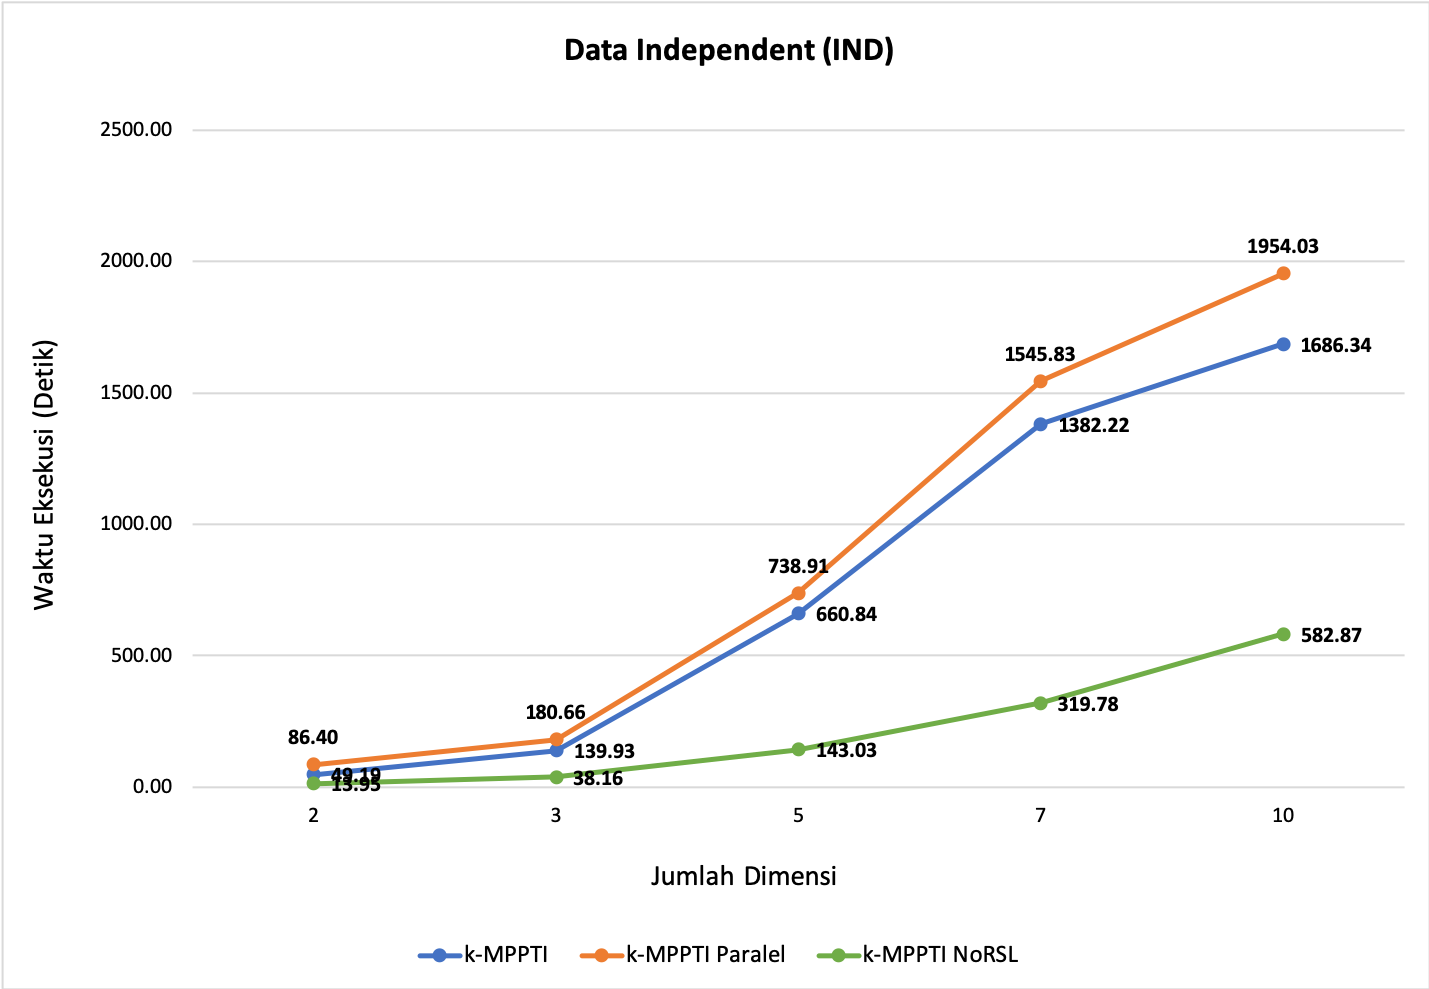
\includegraphics[width=10cm]{assets/img/bab5/grafik-ind-dim-time.png}
	\caption{Grafik pengaruh jumlah dimensi data terhadap waktu komputasi algoritme pada data \textit{independent} (IND)}
	\label{fig:grafik-ind-dim-time}
\end{figure}

\begin{figure}[H]
	\centering
	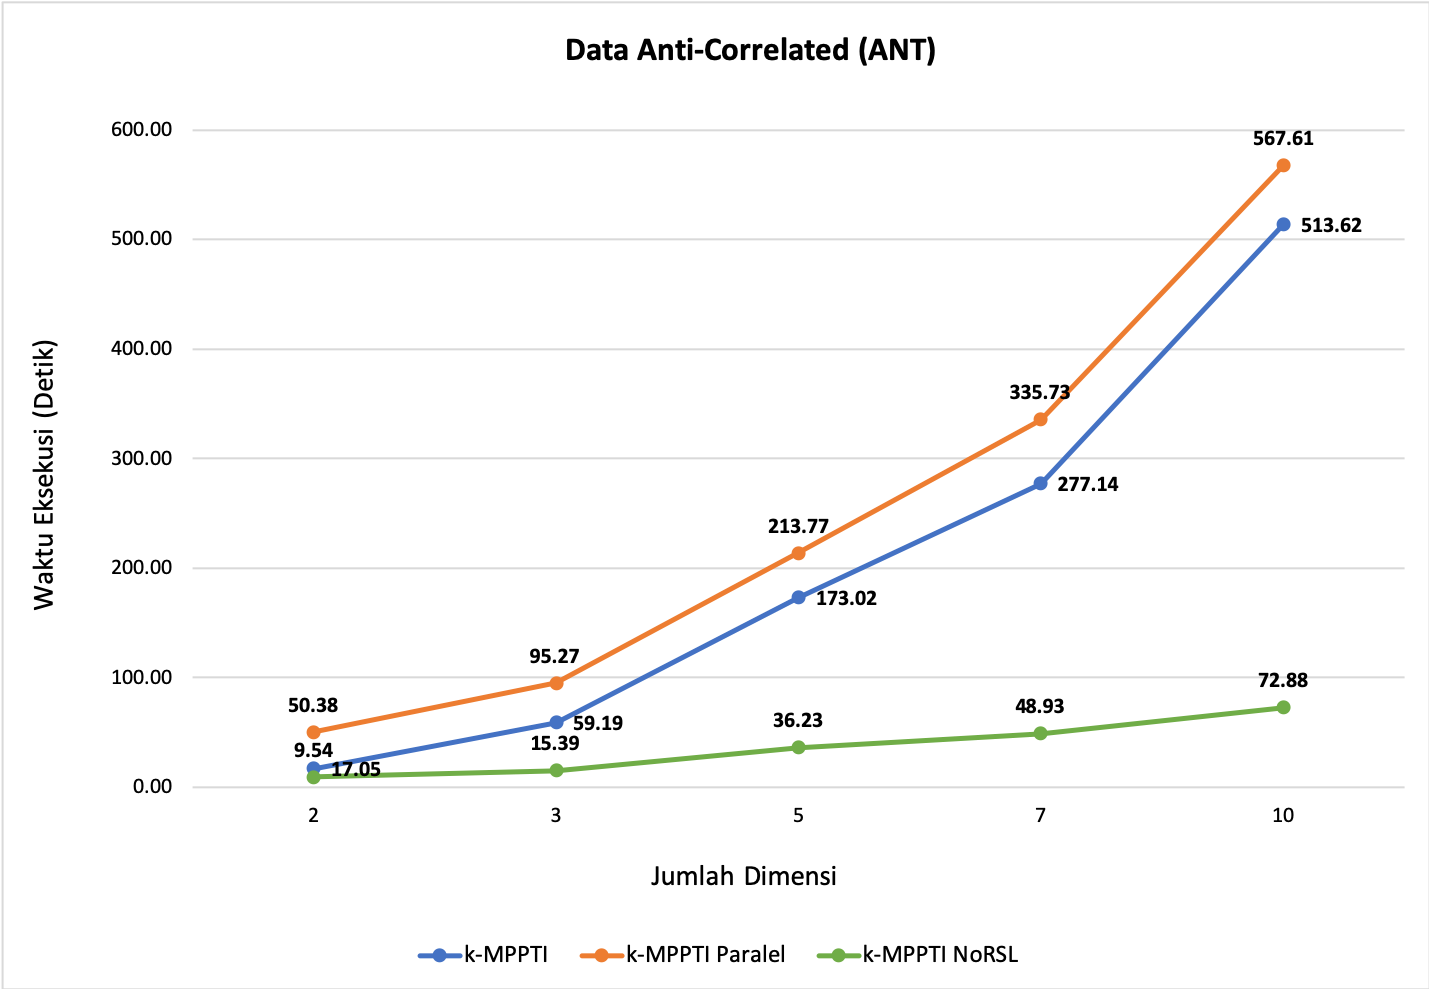
\includegraphics[width=10cm]{assets/img/bab5/grafik-ant-dim-time.png}
	\caption{Grafik pengaruh jumlah dimensi data terhadap waktu komputasi algoritme pada data \textit{anti-correlated} (ANT)}
	\label{fig:grafik-ant-dim-time}
\end{figure}

Jika melihat perbandingan antar data, waktu komputasi pada data \textit{anti-correlated} (ANT) relatif lebih cepat dibandingkan komputasi data \textit{independent} (IND) pada semua algoritme. Namun, data IND memiliki perubahan waktu komputasi yang relatif lebih besar dibandingkan data ANT untuk setiap perubahan jumlah dimensi. Hal ini disebabkan karena nilai atribut pada data IND tidak memiliki keterkaitan satu sama lain, sehingga membutuhkan pemrosesan lebih lama. Jika diperhatikan lebih dalam lagi, semakin besar jumlah dimensi, maka selisih waktu komputasi antara data IND dan ANT juga semakin besar.

\begin{figure}[H]
	\centering
	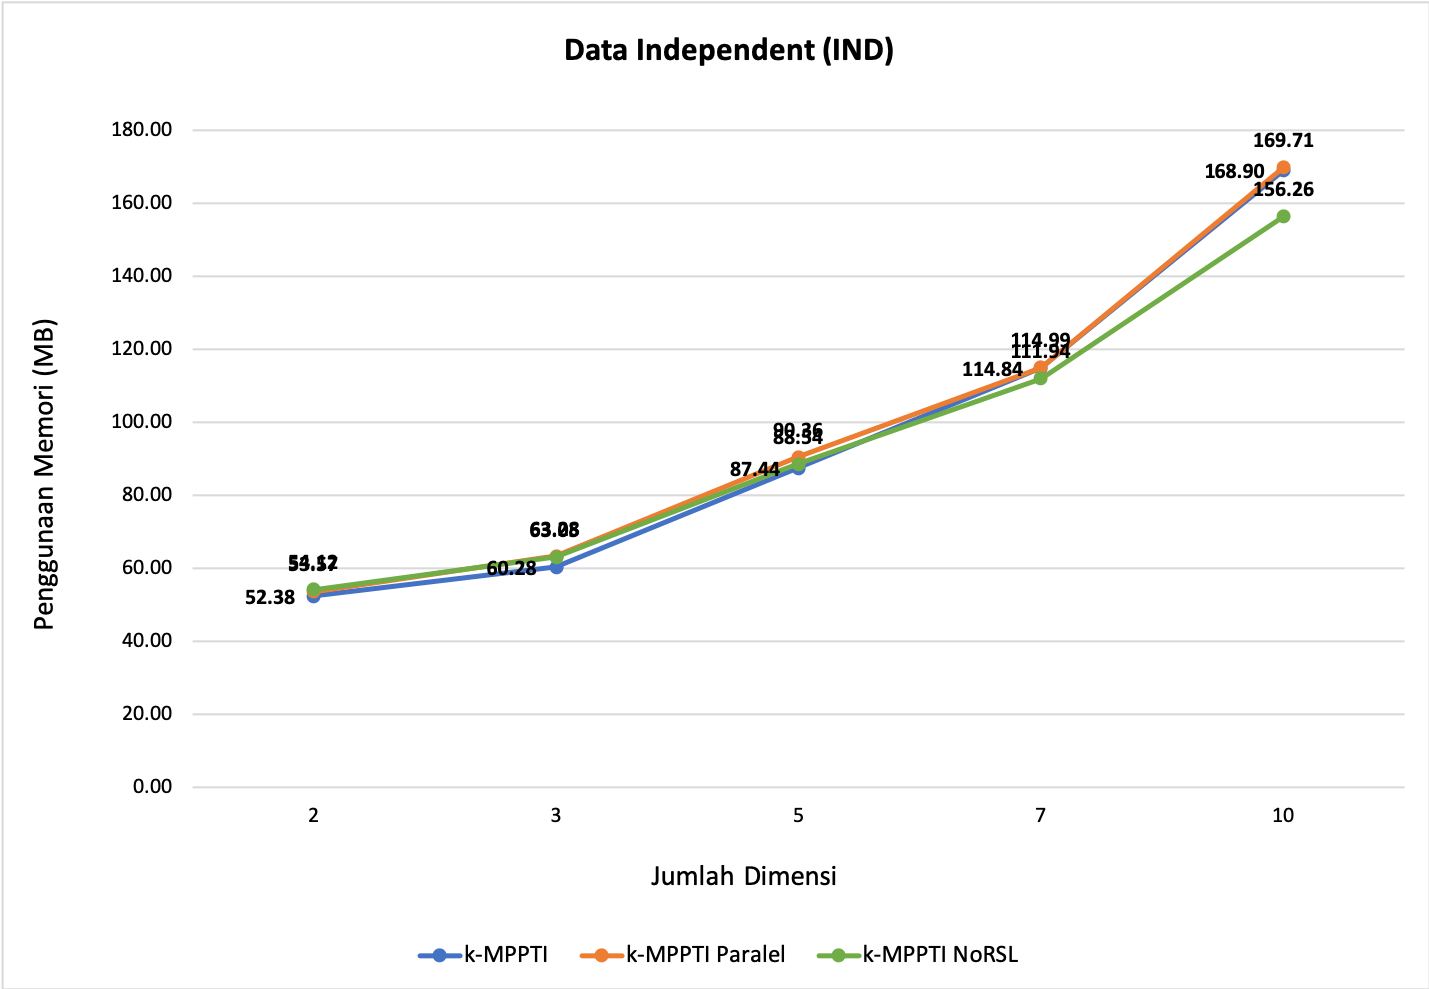
\includegraphics[width=10cm]{assets/img/bab5/grafik-ind-dim-mem.png}
	\caption{Grafik pengaruh jumlah dimensi data terhadap penggunaan memori algoritme pada data \textit{independent} (IND)}
	\label{fig:grafik-ind-dim-mem}
\end{figure}

Di lain sisi, jika melihat perbandingan performa algoritme, algoritme k-MPPTI NoRSL memiliki waktu komputasi paling cepat pada semua jenis data dan algoritme k-MPPTI Paralel memiliki waktu komputasi paling lama pada semua jenis data, walaupun tidak terlalu berbeda jauh dengan waktu komputasi k-MPPTI biasa. Padahal hasil kueri ketiganya mirip dan tidak berbeda jauh (dijelaskan pada sub bagian \ref{hasil-kueri}).

\begin{figure}[H]
	\centering
	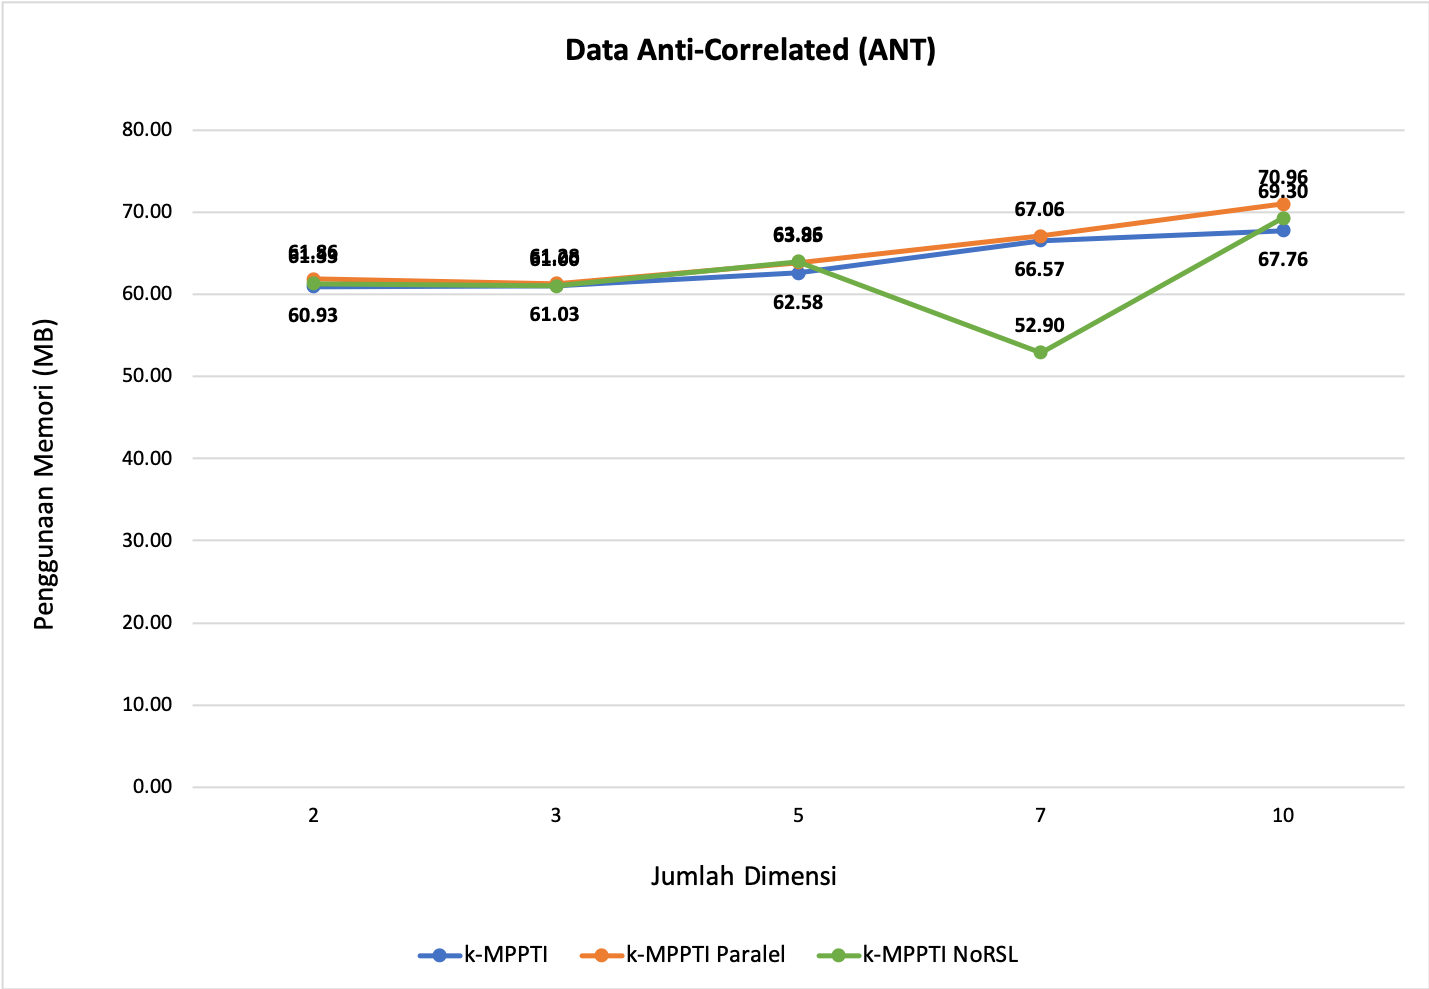
\includegraphics[width=10cm]{assets/img/bab5/grafik-ant-dim-mem.png}
	\caption{Grafik pengaruh jumlah dimensi data terhadap penggunaan memori algoritme pada data \textit{anti-correlated} (ANT)}
	\label{fig:grafik-ant-dim-mem}
\end{figure}

Hasil uji coba pengaruh perubahan jumlah dimensi terhadap penggunaan memori algoritme ditunjukkan oleh Grafik \ref{fig:grafik-ind-dim-mem} dan \ref{fig:grafik-ant-dim-mem}. Dalam grafik tersebut, perubahan memori terjadi secara signifikan pada data IND, namun tidak pada data ANT. Pada data ANT, ada satu hasil yang menunjukkan ketidakstabilan, yakni pada algoritme k-MPPTI NoRSL ketika memproses data dengan tujuh dimensi. Sama seperti sebelumnya, penggunaan memori pada data IND cenderung lebih banyak dibandingkan data ANT.

\pagebreak
\subsubsection{Akurasi Hasil Kueri} \label{hasil-kueri}
\tab Salah satu kekurangan dalam penelitian ini adalah tidak adanya uji coba akurasi terhadap hasil kueri masing-masing algoritme karena tidak ada acuan yang dapat memastikan algoritme yang diimplementasikan benar atau salah. Sehingga, hal yang dapat dilakukan adalah dengan membandingkan hasil kueri antar algoritme. Perbandingan hasil kueri pada masing-masing data ditunjukkan pada Gambar \ref{fig:akurasi1}, \ref{fig:akurasi2}, dan \ref{fig:akurasi3}.

Hasil kueri kedua algoritme pada data \textit{independent} (IND) dengan jumlah 1000 data dengan 5 dimensi 100\% sama, namun memiliki hasil perhitungan kontribusi pasar yang berbeda. Hasil kueri kedua algoritme pada data \textit{anti-correlated} (ANT) dengan jumlah 4000 data dengan 3 dimensi memiliki anggota yang sama, namun peringkat dan hasil perhitungan kontribusi pasarnya yang berbeda. Sedangkan hasil kueri kedua algoritme pada data \textit{forest cover type} dengan jumlah 1000 data dengan 3 dimensi memiliki perbedaan yang signifikan karena memiliki satu anggota yang berbeda dan hasil peringkat satu pada komputasi k-MPPTI tidak menjadi hasil pada komputasi k-MPPTI NoRSL.

\begin{figure}[H]
	\centering
	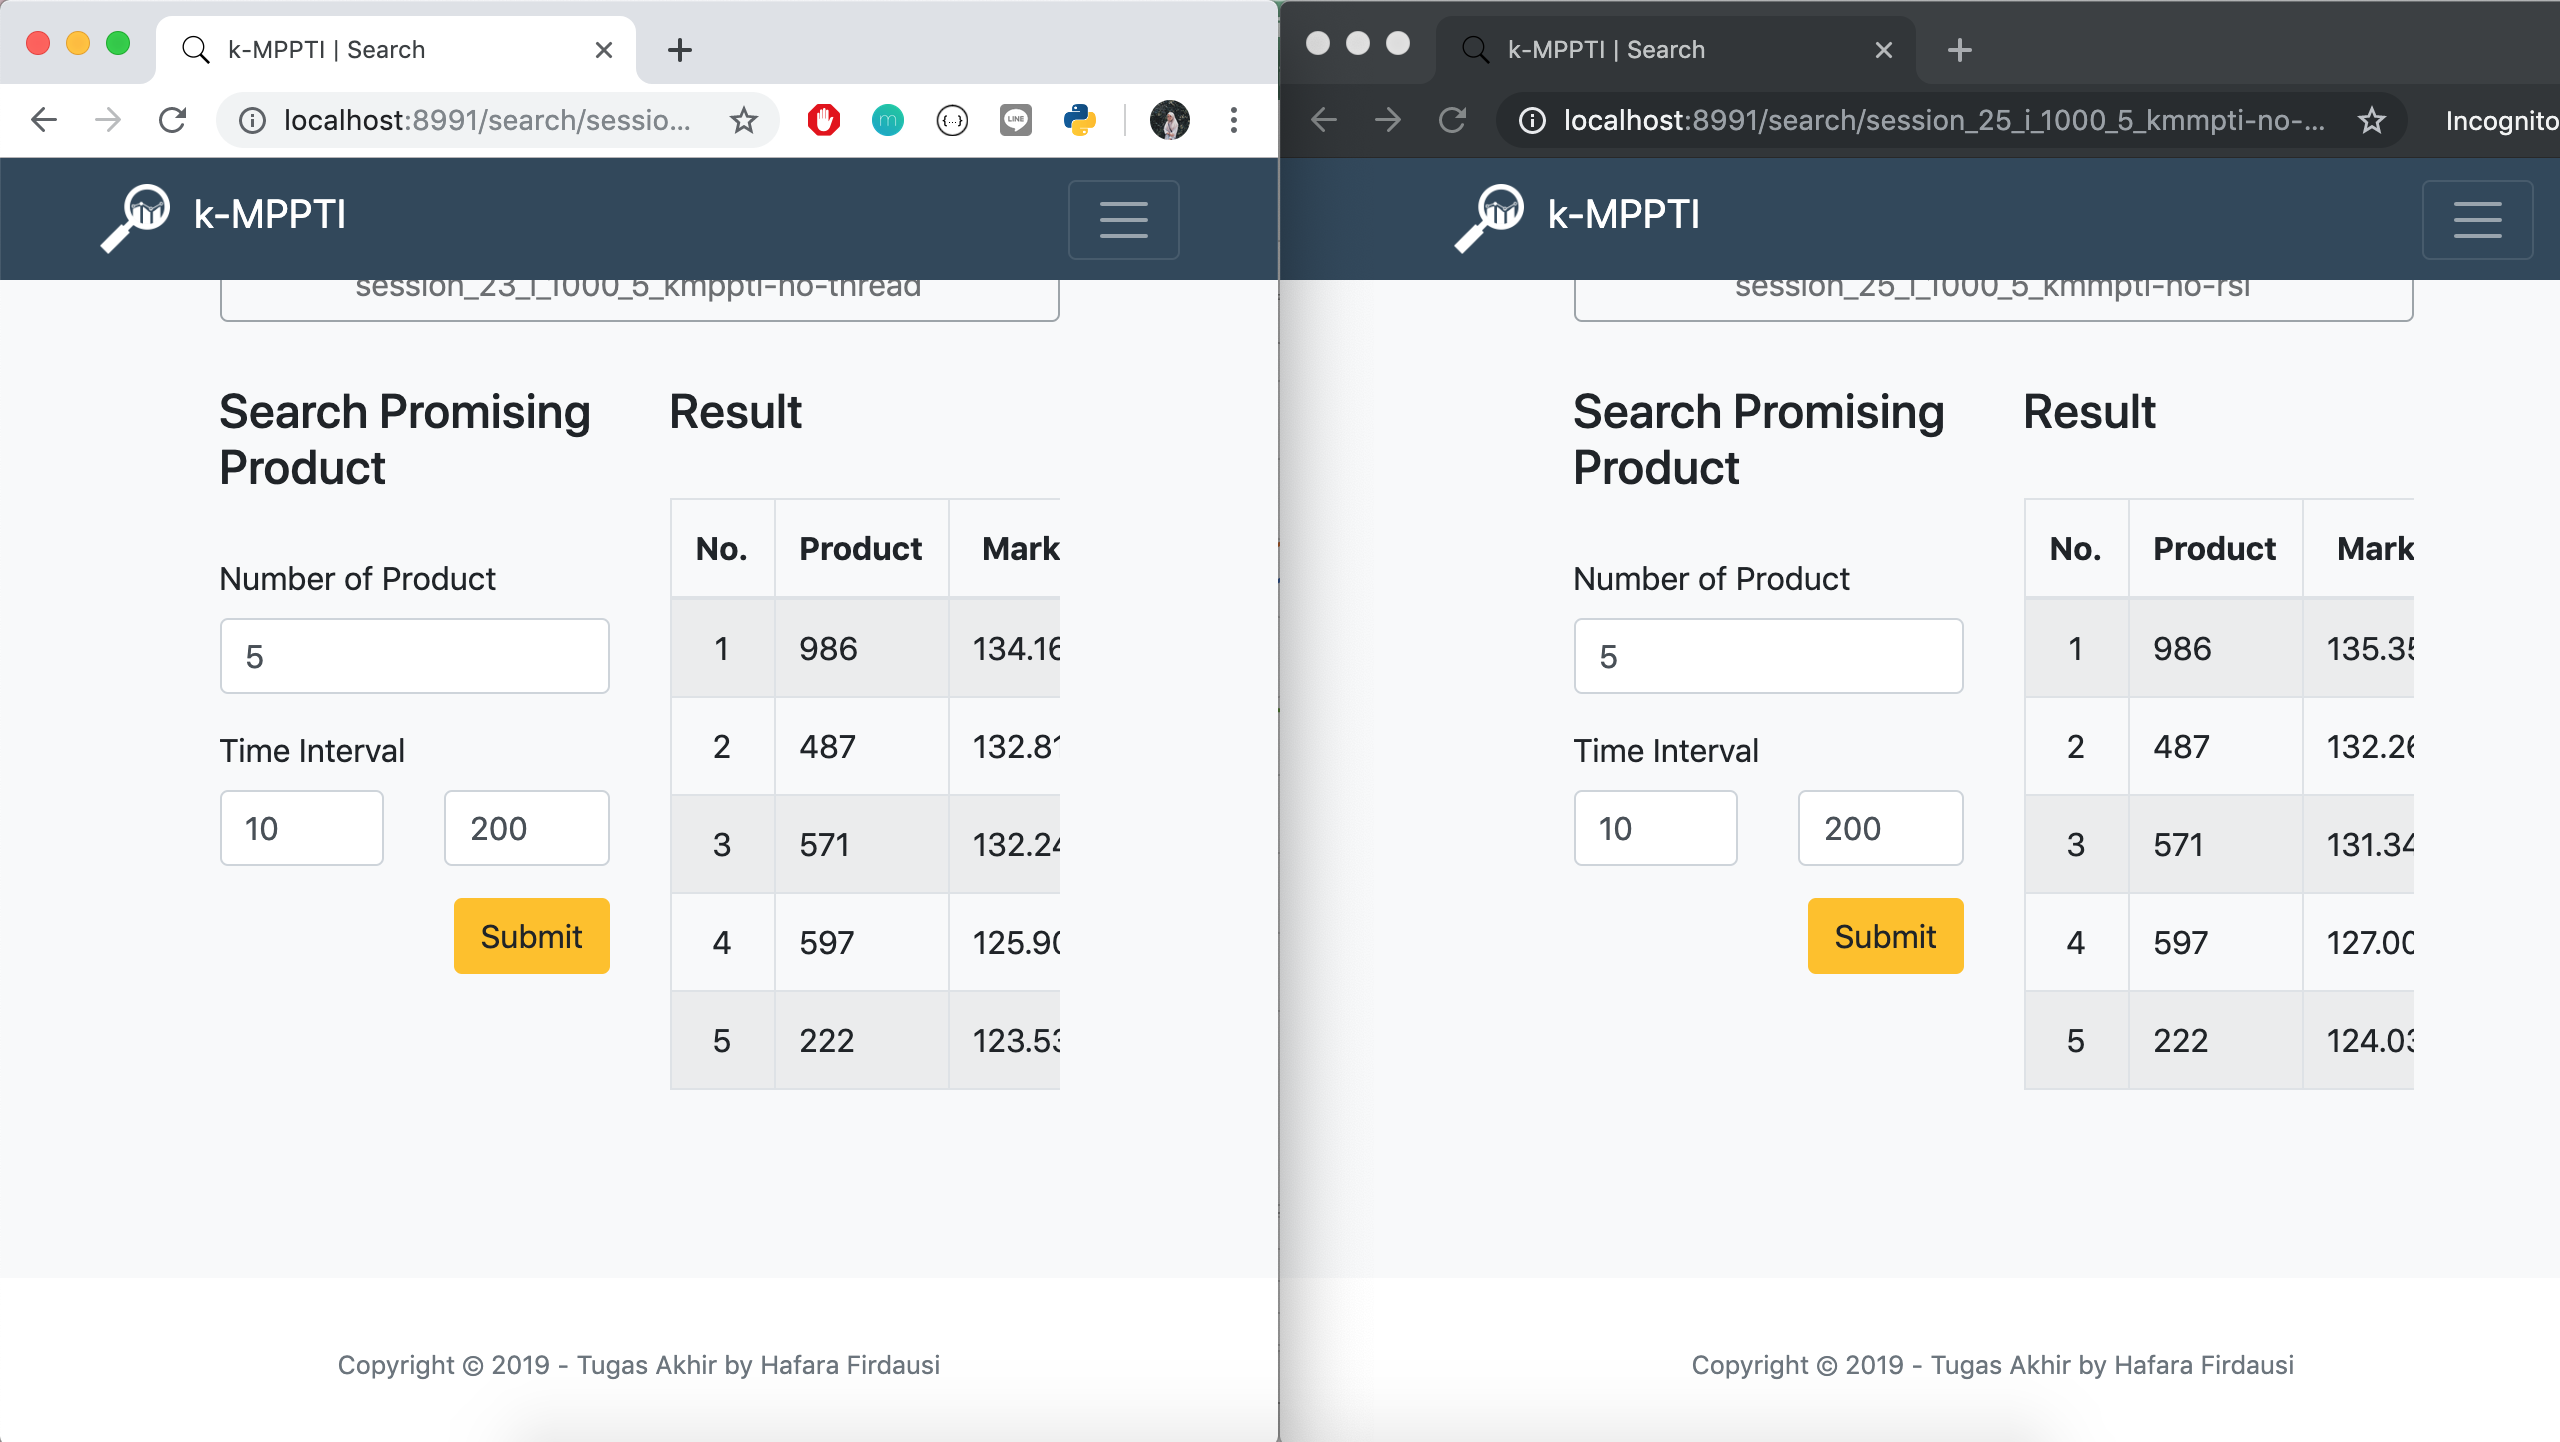
\includegraphics[width=10cm]{assets/img/bab5/pengujian-akurasi1.png}
	\caption{Pengujian akurasi hasil kueri pada data \textit{independent} (IND)}
	\label{fig:akurasi1}
\end{figure}

\begin{figure}[H]
	\centering
	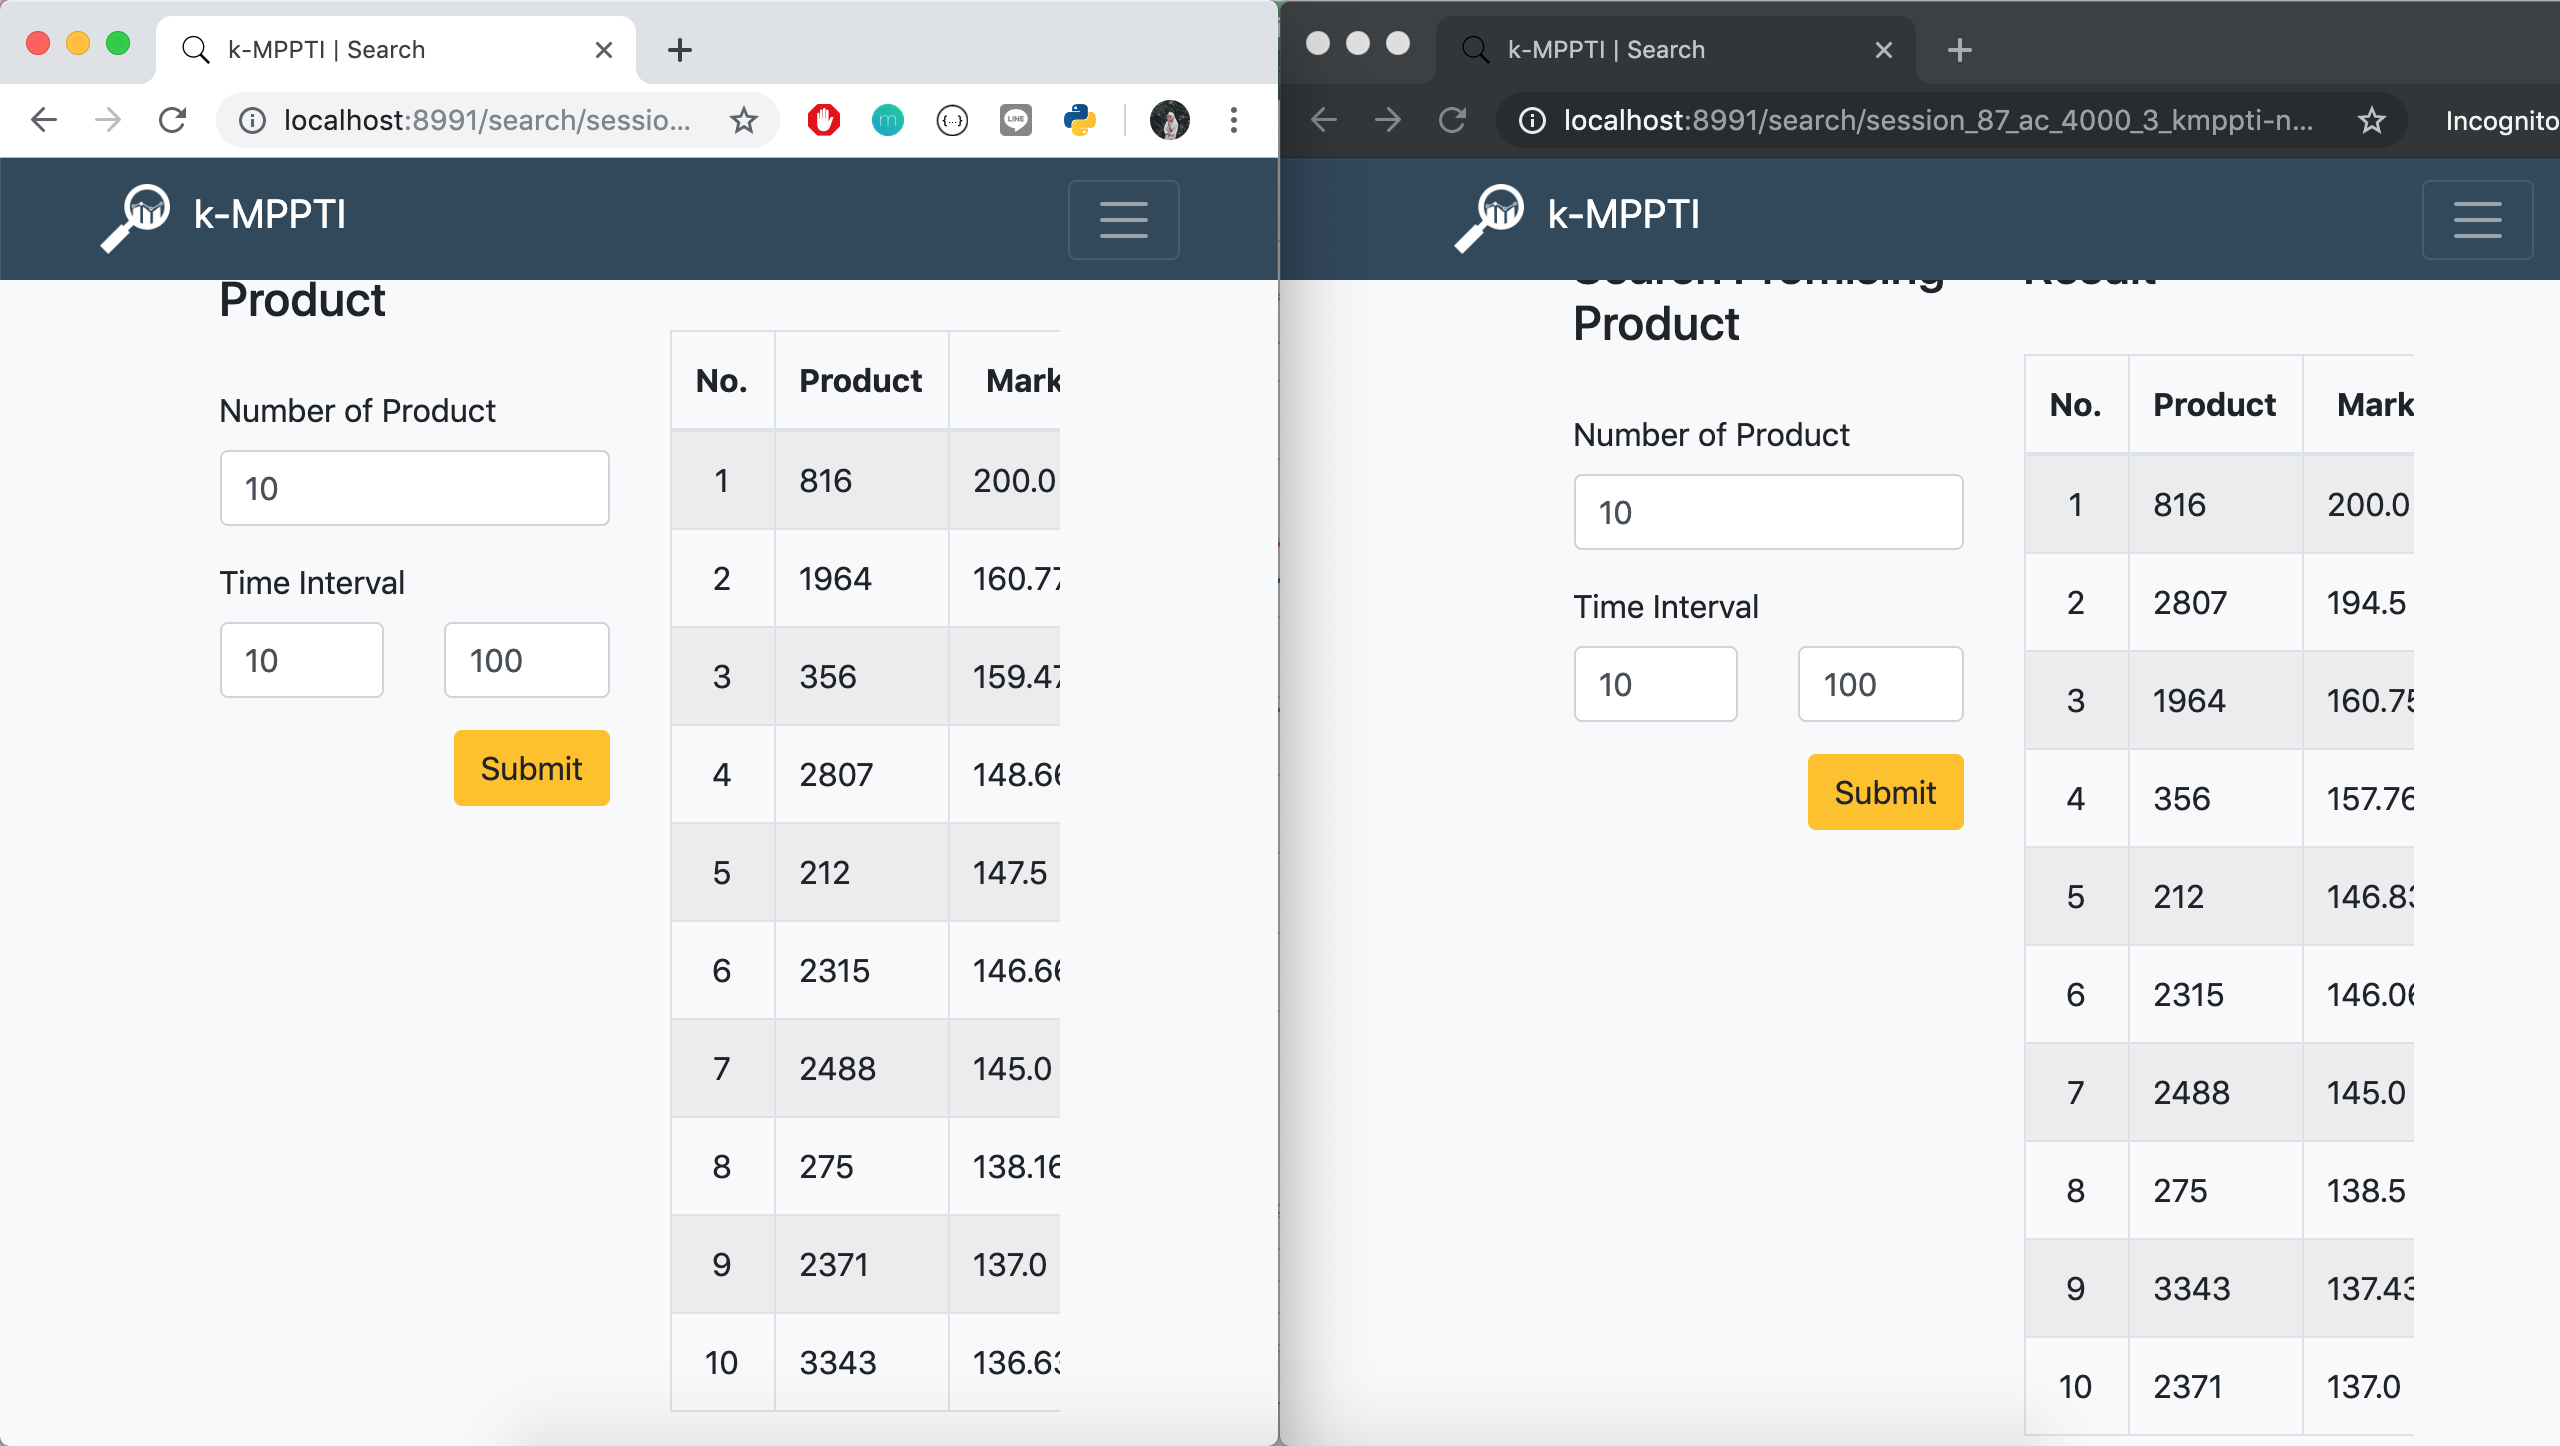
\includegraphics[width=10cm]{assets/img/bab5/pengujian-akurasi3.png}
	\caption{Pengujian akurasi hasil kueri pada data \textit{anti-correlated} (ANT)}
	\label{fig:akurasi3}
\end{figure}

\begin{figure}[H]
	\centering
	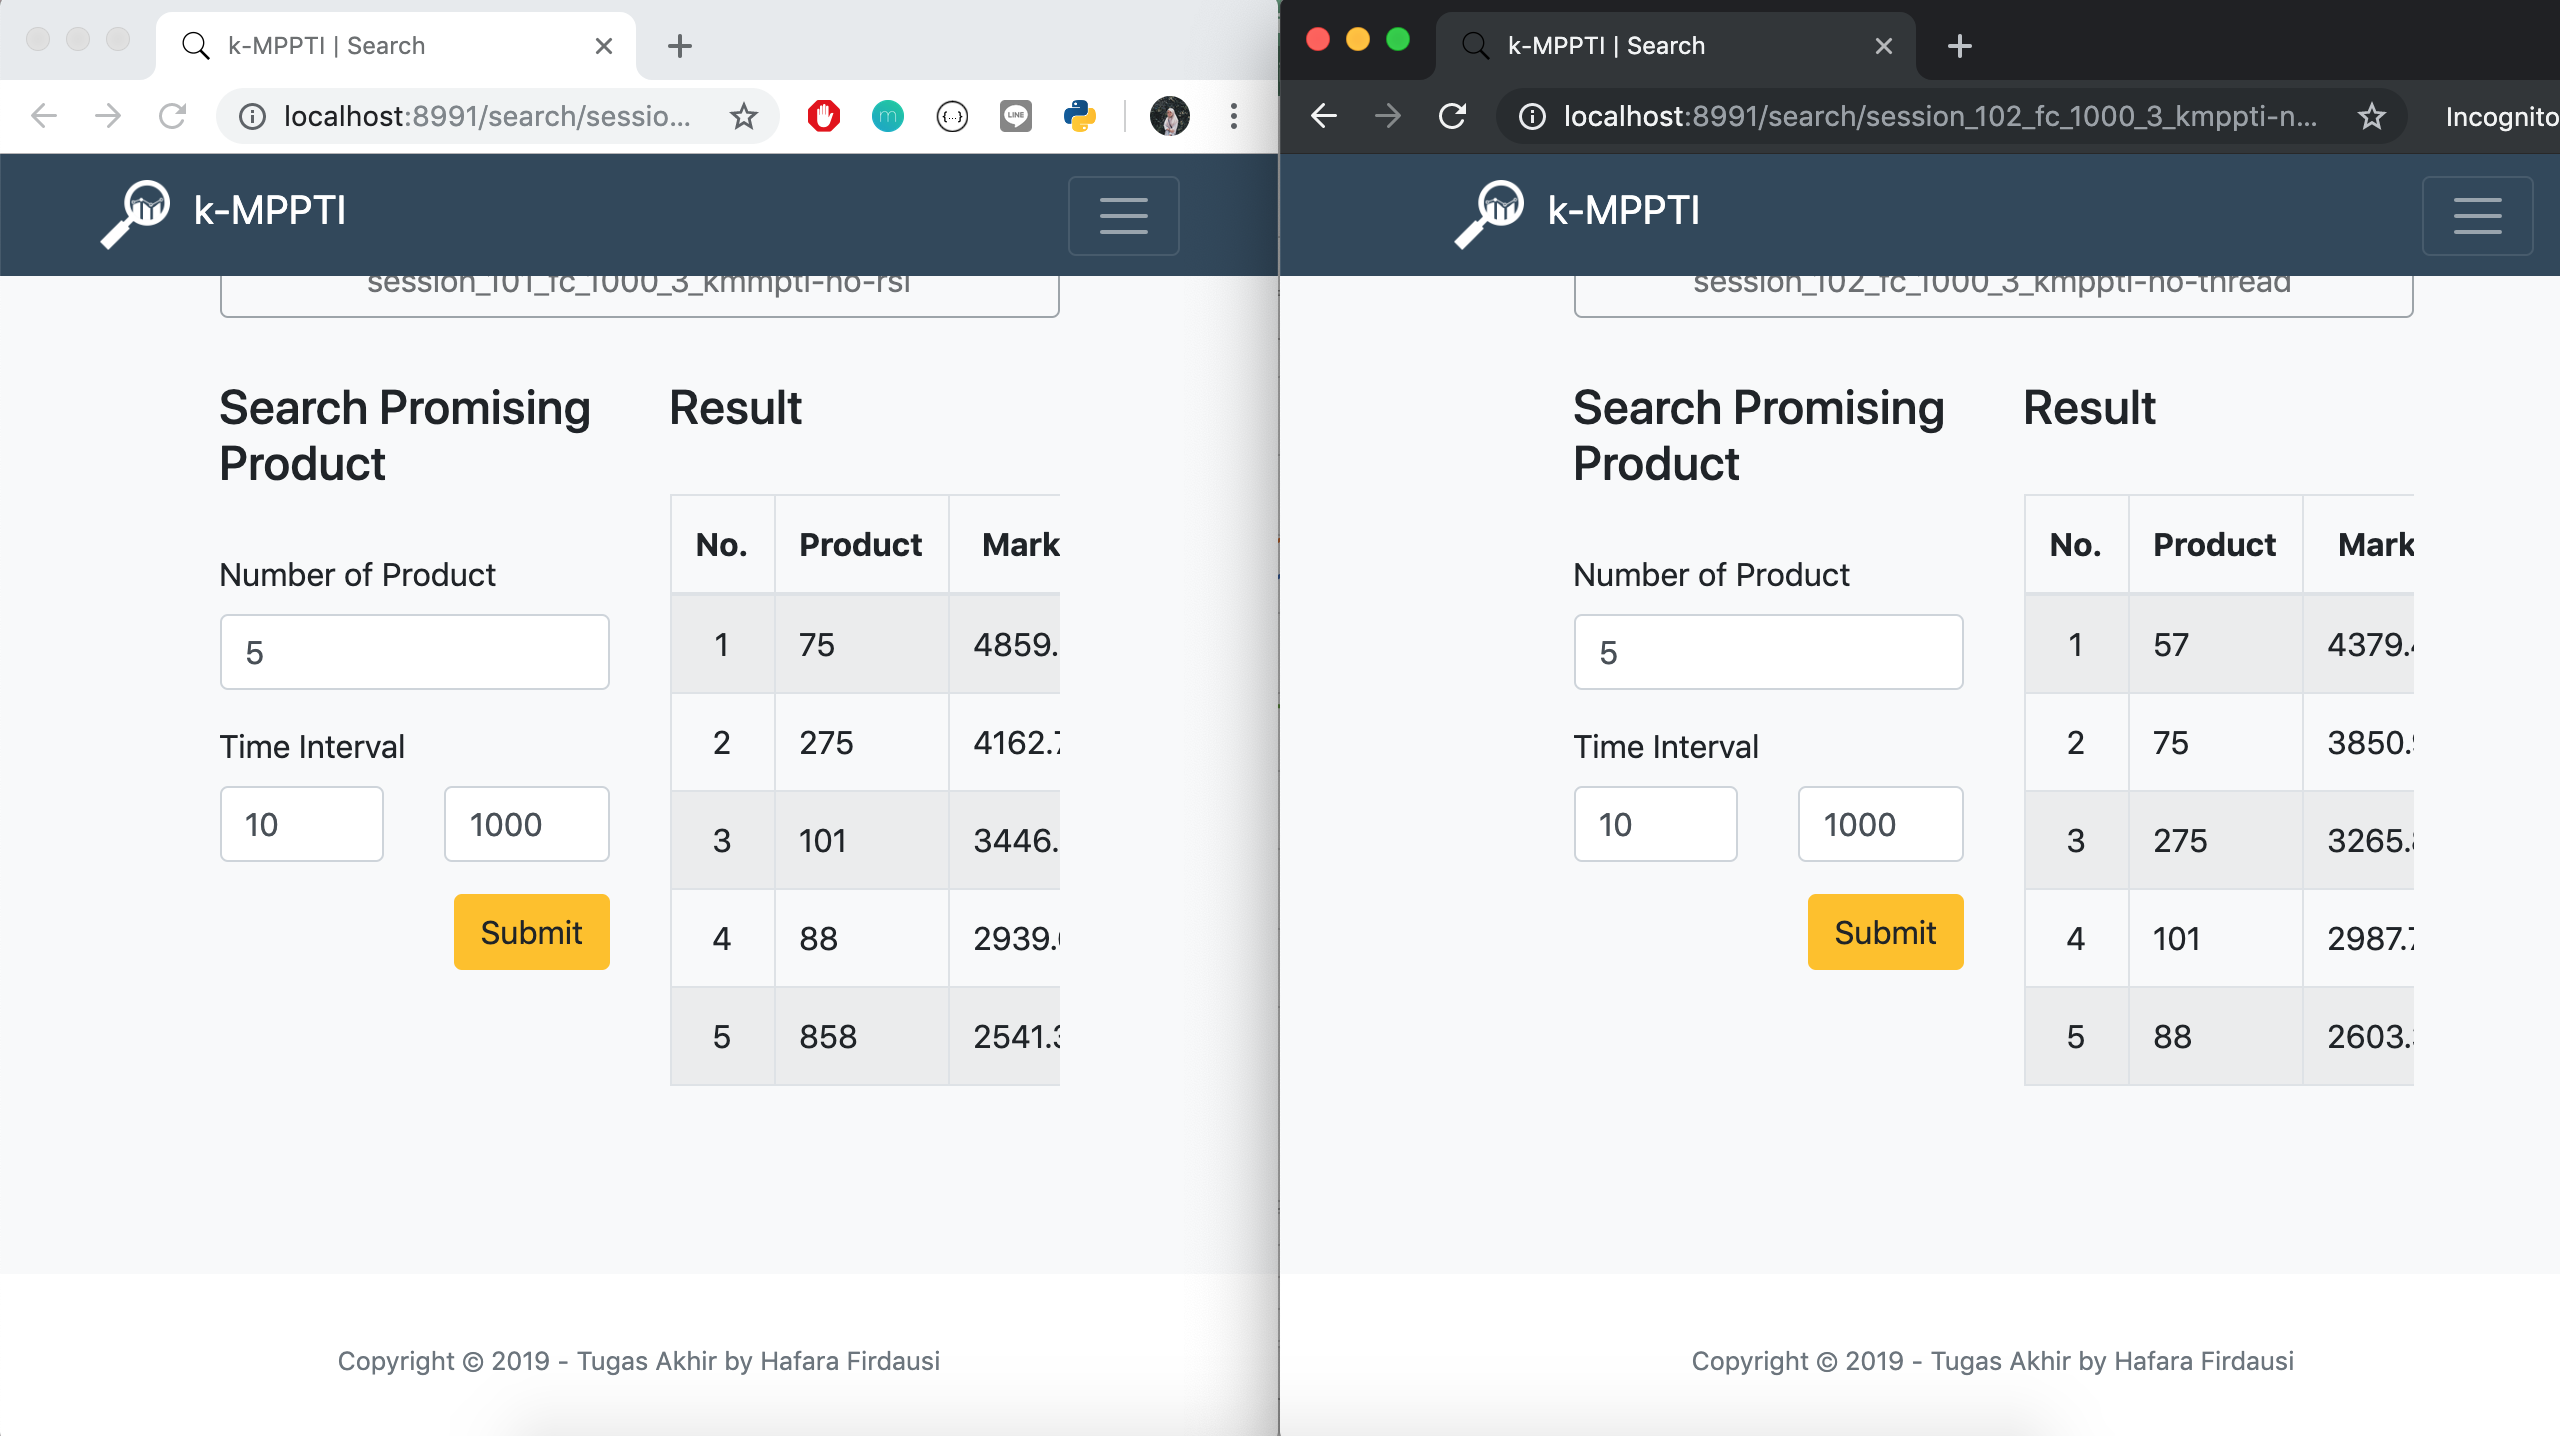
\includegraphics[width=10cm]{assets/img/bab5/pengujian-akurasi2.png}
	\caption{Pengujian akurasi hasil kueri pada data \textit{Forest Cover Type} (FC)}
	\label{fig:akurasi2}
\end{figure}

	\chapter{KESIMPULAN DAN SARAN}\label{chap:kesimpulan-saran}

\tab Pada bab ini dijelaskan mengenai kesimpulan dan saran dari hasil uji coba yang telah dilakukan.

\section{Kesimpulan}

\tab Dari proses desain hingga uji coba, dapat diambil beberapa hasil sebagai berikut:

\begin{enumerate}
	\item Tugas akhir ini mengusulkan struktur data grid indeks dan metode $ CSd_\varepsilon $ untuk pengolahan \textit{skyline query} pada \textit{uncertain data streaming} oleh titik bergerak dan objek tidak bergerak. Struktur data grid indeks memecah struktur data graf tradisional menjadi sel-sel yang berisi \textit{node}, \textit{edge}, dan objek. Penyimpanan objek dalam bentuk \textit{SW-Tree} pada setiap \textit{node} membuat proses komputasi lebih cepat.
	
	\item Biaya komputasi pada metode $ CSd_\varepsilon $ jauh lebih baik dibandingkan metode \textit{naive} dari sisi waktu komputasi dan penggunaan memori. Komputasi metode $ CSd_\varepsilon $ lebih cepat 600 kali dibandingkan metode \textit{naive}. Dari sisi penggunaan memori, metode $ CSd_\varepsilon $ lebih hemat 1500 kali dibandingkan metode \textit{naive}.
\end{enumerate}

\section{Saran}

\tab Berikut beberapa saran terkait pengembangan lebih lanjut:

\begin{enumerate}
	\item Pendefinisian jarak $ d_\varepsilon $ dapat dilakukan secara dinamis. Apabila pencarian objek dengan jarak $ d_\varepsilon $ tidak menemukan hasil yang diminta, jarak $ d_\varepsilon $ dapat diperbesar secara dinamis hingga mendapatkan hasil yang sesuai.
	\item Pengembangan algoitma untuk memproses objek \textit{uncertain} yang dapat bergerak secara dinamis.
	\item Pada algoritme ini proses pembaruan \textit{instance} dari \textit{uncertain} objek dilakukan dengan menghapus dan menambahkan objek baru. Hal ini tentunya tidak efisien. Diperlukan algoritme pembaruan objek agar lebih efisien dalam hal waktu komputasi dan penggunaan memori.
\end{enumerate}




	
	\renewcommand\chaptername{LAMPIRAN}
	\appendix
	\begin{thebibliography}{9}
	\bibitem{kmpp}
	M. S. Islam and C. Liu, \textbf{Know Your Customer: Computing K-Most Promising Products}, The VLDB Journal, pp. 545–570, 2016.
	
	\bibitem{dynamic-skyline}
	D. Papadias, Y. Tao, G. Fu and B. Seeger, \textbf{Progressive Skyline Computation in Database Systems}, ACM Transactions on Database Systems, Vol. 30, No. 1, pp. 41–82, 2005.
	
	\bibitem{dynamic-skyline-2}
	L. Zou, L. Chen, M. T. Özsu and D. Zhao, \textbf{Dynamic Skyline Queries in Large Graphs}, DASFAA'10 Proceedings of the 15th International Conference on Database Systems for Advanced Applications - Volume Part II, pp. 62-78, 2010.
	
	\bibitem{reverse-skyline}
	E. Dellis and B. Seeger, \textbf{Efficient Computation of Reverse Skyline Queries}, VLDB Endowment, pp. 291-302, 2007.
	
	\bibitem{interval-skyline}
	B. Jiang and J. Pei, \textbf{Online Interval Skyline Queries on Time Series}, IEEE International Conference on Data Engineering, pp. 1036-1047, 2009.
	
	\bibitem{skyline}
	S. Borzsonyi, D. Kossmann and K. Stocker, \textbf{The Skyline Operator}, In: ICDE, pp. 421-430, 2001.
	
	\bibitem{influence}
	X. Wu, Y. Tao, R. C.-W. Wong, L. Ding and J. X. Yu, \textbf{Finding the Influence Set through Skylines}, EDBT, pp. 1030-1041, 2009.
		
\end{thebibliography}

	\backmatter
	\chapter{BIODATA PENULIS}
\begin{wrapfigure}{l}{0.3\textwidth}
	\includegraphics[width=0.29\textwidth]{biodata/img/hf.png}
\end{wrapfigure}

\textbf{Hafara Firdausi}, lahir di Surabaya pada tanggal 19 September 1998. Penulis merupakan anak pertama dari 3 bersaudara. Penulis telah menempuh pendidikan formal di SD Negeri Gelam 1 Candi (2004-2010), SMP Negeri 1 Sidoarjo (2010-2013), dan SMA Negeri 1 Sidoarjo (2013-2015). Kemudian, penulis melanjutkan studi kuliah program sarjana di Departemen Informatika, Institut Teknologi Sepuluh Nopember Surabaya.\\
\tab Selama menempuh pendidikan di Informatika ITS, penulis pernah menjadi asisten dosen dan praktikum untuk mata kuliah Jaringan Komputer (2017-2018) dan Sistem Operasi (2019), serta menjadi Administrator Laboratorium Arsitektur dan Jaringan Komputer (AJK). Selain itu, penulis juga aktif dalam kegiatan organisasi dan kepanitiaan, antara lain menjadi Badan Pengurus Harian I 3D (Desain, Dekorasi, dan Dokumentasi) Schematics ITS 2017, staff dan staff ahli Departemen Media Informasi Himpunan Mahasiswa Teknik Computer-Informatika (HMTC) ITS, dan Panitia Gemastik ke-11 Bidang Keamanan Jaringan dan Sistem Informasi (KJSI). Penulis dapat dihubungi melalui surel di  \texttt{hafarafirdausi@gmail.com}.
\end{document}

